%%% BkgModelling %%%
\chapter{Background Modeling and Estimations}

The modeling of major background processes, such as \Wjets and top quark pair (\ttbar) productions, is examined in this section. 
Since \Zjets production has no meaningful contribution to the \Vjets backgrounds in the \olep channel, we focus solely on \Wjets for simplicity. 
Initially, attention is directed towards the study of mismodeling in the invariant mass of the VBS Tag Jets, denoted as \mjjtag, specifically within \Wjets events in the \olep channel. 
Subsequently, various control regions for \Wjets and \ttbar backgrounds are established. These regions are instrumental in validating the modeling and constraining the normalization based on data.

%%%
\section{Reweighting for the Tag Jets}
%%\subsection{Re-weighting for the tagging jets}
\label{subsec:mjj_reweight}


The invariant mass of the two selected Tag Jets is known to be mismodeled in the Sherpa 2.2.1 V+jets samples, a critical variable due to the forward topology of our final state. Consequently, we applied a linear reweighting procedure to the \Wjets
%and \Zjets 
MC samples, aligning with data in the CRs.

\label{subsec:mjj_reweight_1lep}

%%%The modelling of the \Wjets background for the 1-lepton channel,
%%%is studied in this subsection.
%%%In Figure \ref{fig:mjjReweight1LepMjjDistBefore} the $\Mtag$ distributions for the merged and resolved regions are plotted.
%%%Similarly to the 0- and 2-lepton channels,
%%%a clear mis-modelling between the main background source and data is also observed in the 1-lepton channel.
%%%In order to account for this mis-modelling, a reweighting for the \Wjets MC is derived.

This section examines the \Wjets background modeling for the 1-lepton channel. 
Figure \ref{fig:mjjReweight1LepMjjDistBefore} shows the $\Mtag$ distributions for both merged and resolved regions, highlighting noticeable discrepancies between the primary background source and observed data. 
%To address this mis-modeling, a reweighting of the \Wjets MC samples is implemented.

To correct the mis-modeling, which we assume varies linearly with \mjjtag, we apply this reweighting formula to the \Wjets events:

\begin{equation}
  w(m_{jj}^{tag}) =  p_0 + p_1 * m_{jj}^{tag} ,
\end{equation}
%
where $p_0$ and $p_1$
are coefficients calculated independently for both merged and resolved regions, and $w(m_{jj}^{tag})$ will be the re-weighted applied. 
After determining these values from control regions (see Table \ref{tab:mjjReweight1LepRegions}), we apply the corrections to the respective signal regions.
For both merged and resolved scenarios, we obtain $p_0$ and $p_1$ by fitting the Sherpa \Wjets model-to-data ratio, after subtracting non-\Wjets backgrounds. 

%For the merged case, we perform a single fit on \mjjtag across the entire $m_{J}$ range, enhancing the statistical reliability of the results.
For the merged case, a single fit is applied to the entire \mjjtag distribution without subdividing the sample based on the $m_{J}$ range. This approach simplifies the analysis while maintaining statistical robustness, as illustrated in Figure \ref{fig:mjjReweight1LepMer}.

In the resolved case, the fit to \mjjtag is done within specific $m_{jj}^{sig}$ bins ([50,60,70,100,120,150,200,300] GeV) to assess variations in reweighting factors. This approach involves segmenting both MC and data samples by $m_{jj}^{sig}$, as illustrated in Figure \ref{fig:mjjReweight1LepResPtBins}. After determining the values of $p_0$ and $p_1$ across various $m_{jj}^{sig}$ bins, these are then fitted to obtain the definitive reweighting factors for the signal region's $m_{jj}^{sig}$, as illustrated in Figure \ref{fig:mjjReweight1LepResFit}. This is followed by an interpolation from the control to the signal region.

The studies encompassed all data periods and corresponding MC campaigns (mc16a, mc16d, and mc16e). To verify consistency across different data periods and pileup conditions, these analyses were repeated for each MC campaign, with outcomes presented in Figure \ref{fig:mjjReweight1LepResTotal}.
A slight dependence on the MC period was observed, but the improvement from adjusting the \mjjtag reweighting for each period was minimal. Thus, we used the combined period results for the final analysis.

Table ~\ref{tab:1lepReweighting} shows the final parameters derived for the \olep channel.
The \mjjtag distributions for the three SRs before and after reweighting are depicted in Figures \ref{fig:mjjReweight1LepMjjDistBefore} and \ref{fig:mjjReweight1LepMjjDistAfter}, respectively.

\begin{table}[ht]
    \centering
    \caption{Definition of control regions used to derive \Wjets reweighting factors.}
    \begin{tabular}{|c|c|}
        \hline
        \multirow{2}{4em}{Resolved} & pass Resolved Selection (NoMassWindowCut)  \\
         & BjetVeto  \\
         \hline
        \multirow{2}{4em}{Merged} &  pass Merged Selection (NoMassWindowCut) \\
        & BjetVeto  \\
         \hline
    \end{tabular}
%    \caption{Definition of control regions used to derive \Wjets reweighting factors.}
    \label{tab:mjjReweight1LepRegions}
\end{table}

%%Table ~\ref{tab:1lepReweighting} shows the final parameters derived for the \olep channel.

\begin{table}[ht]
     \centering
     \caption{1-lepton $m(jj)^\text{tag}$ reweighting factors.}
     \label{tab:1lepReweighting}
         \begin{tabular}{ |c|c|c| }
\hline
Parameter & Merged CRVjet & Resolved CRVjet  \\
\hline
$p_{0}$ (slope) [$\GeV^{-1}$] & $(-51.4 \pm 2.9)10^{-5}$ &  $(-14.4 \pm 6.1)10^{-5}$ \\
 \hline
$p_{1}$ (constant)  & $1.47 \pm 0.03$ & $1.13 \pm 0.02$ \\
\hline
         \end{tabular}
\end{table}

\clearpage
\begin{figure}[ht]
    \centering
    \begin{subfigure}[b]{0.3\textwidth}
        \centering
        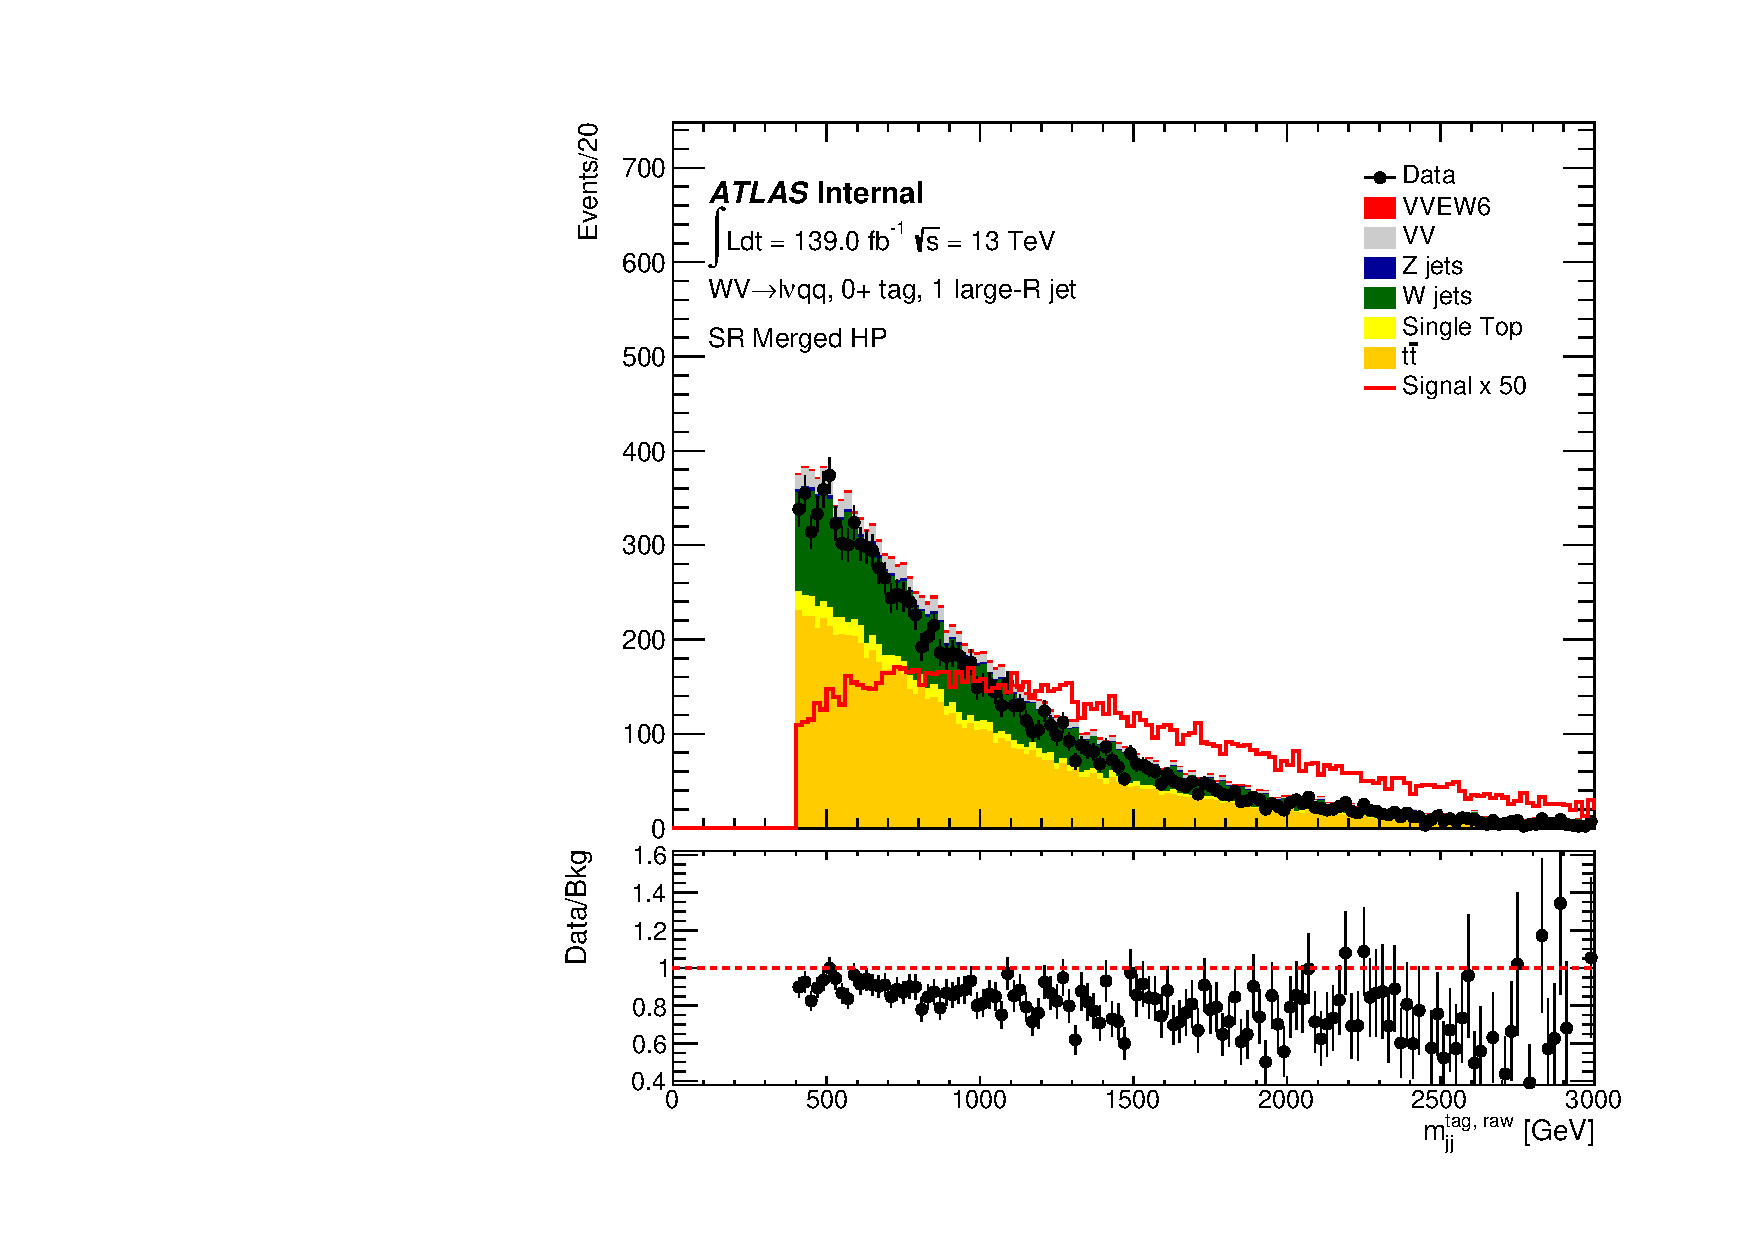
\includegraphics[width=\textwidth]{figures/mjjreweight1lep/SR_50/stacked_plot_merged_tagMjj_MjjWeightMerged.pdf}
        \caption{Merged HP SR RAW}
        \label{fig:MC16ADE_Merged_HP_SR_Before}
    \end{subfigure}
    \hfill
    \begin{subfigure}[b]{0.3\textwidth}
        \centering
        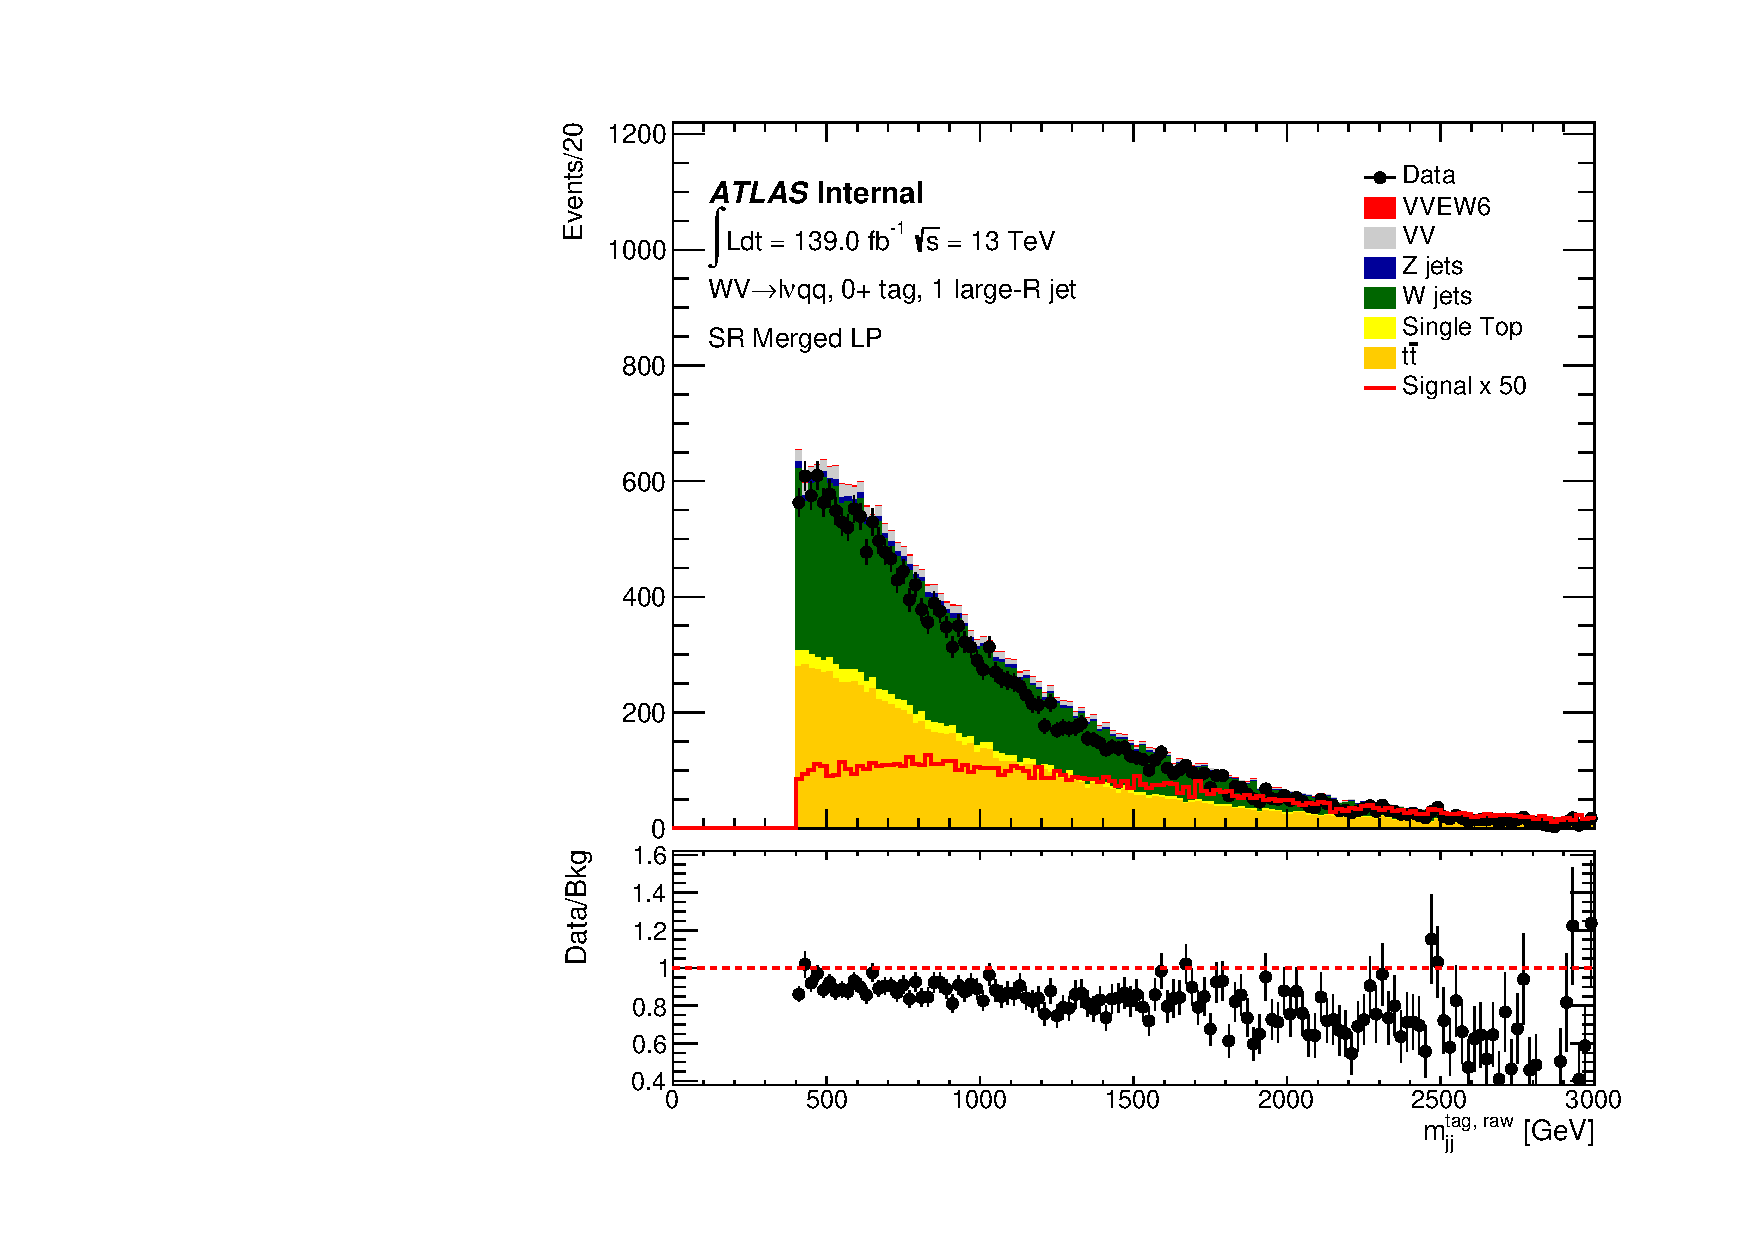
\includegraphics[width=\textwidth]{figures/mjjreweight1lep/SR_80/stacked_plot_merged_tagMjj_MjjWeightMerged.pdf}
        \caption{Merged LP SR RAW}
        \label{fig:MC16ADE_Merged_LP_SR_Before}
    \end{subfigure}
    \hfill
    \begin{subfigure}[b]{0.3\textwidth}
        \centering
        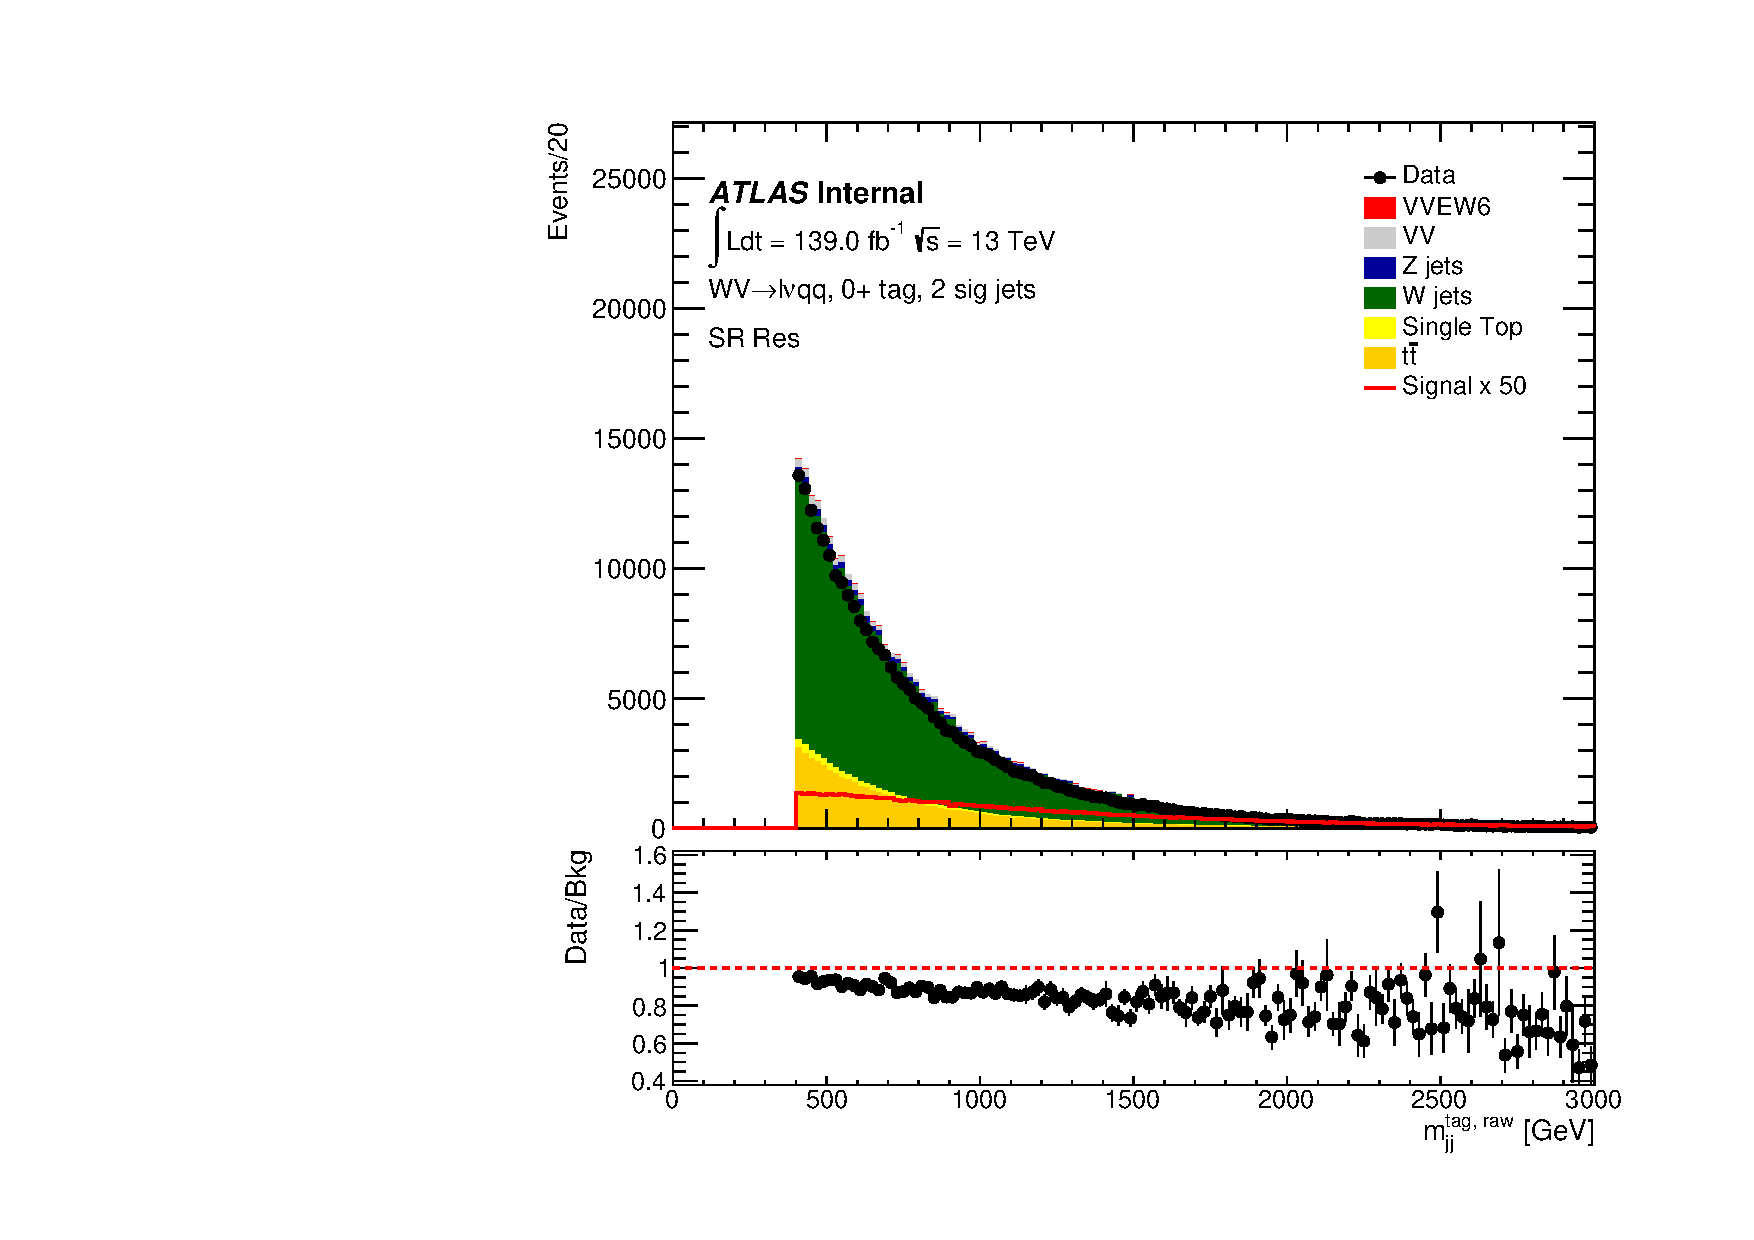
\includegraphics[width=\textwidth]{figures/mjjreweight1lep/SR_Res/stacked_plot_resolved_tagMjj_MjjWeightResolved.pdf}
        \caption{Resolved SR RAW}
        \label{fig:MC16ADE_Resolved_SR_Before}
    \end{subfigure}
    \caption{\(\mjjtag\) distributions without any corrections in the signal regions.}
    \label{fig:mjjReweight1LepMjjDistBefore}
\end{figure}

\begin{figure}[ht]
    \centering
    \begin{subfigure}[b]{0.3\textwidth}
        \centering
        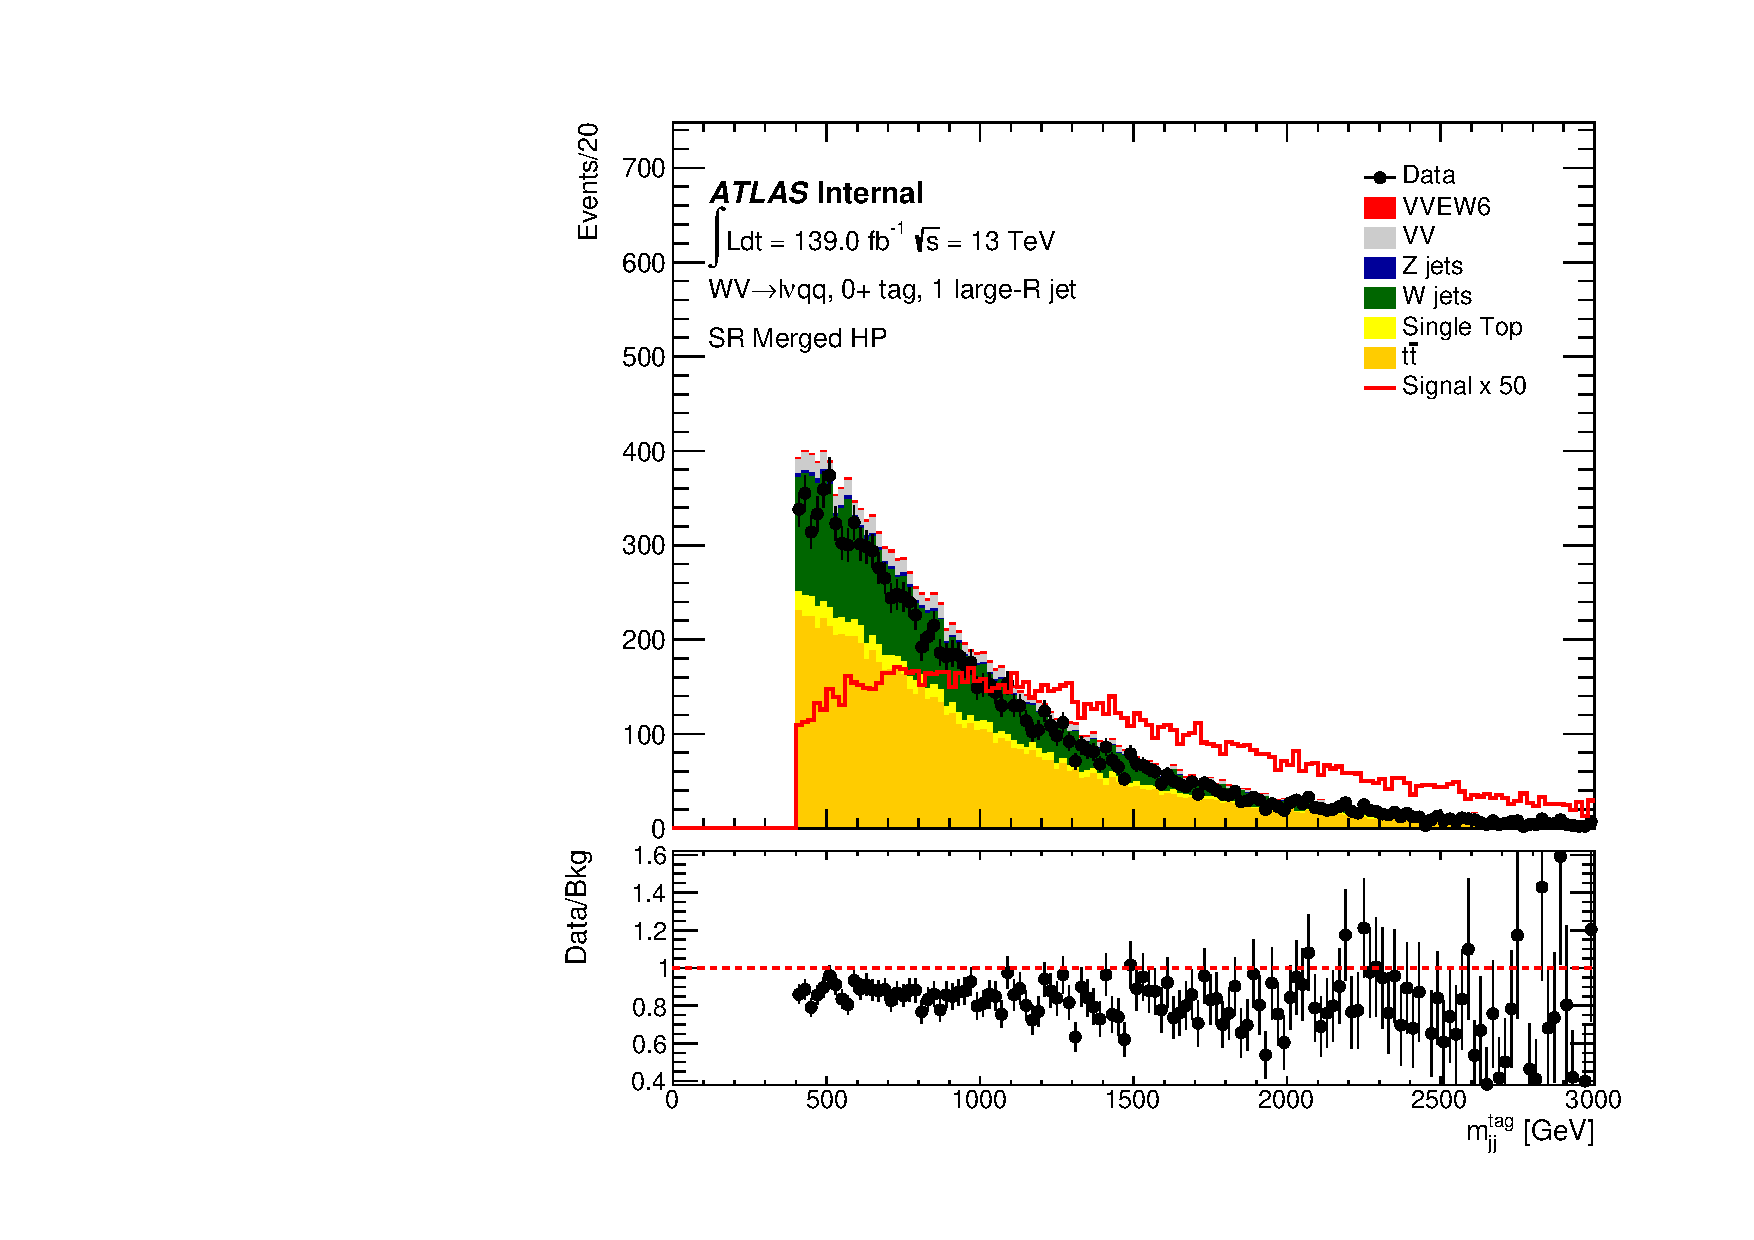
\includegraphics[width=\textwidth]{figures/mjjreweight1lep/SR_50/stacked_plot_merged_tagMjj.pdf}
        \caption{Merged HP SR}
        \label{fig:MC16ADE_Merged_HP_SR}
    \end{subfigure}
    \hfill
    \begin{subfigure}[b]{0.3\textwidth}
        \centering
        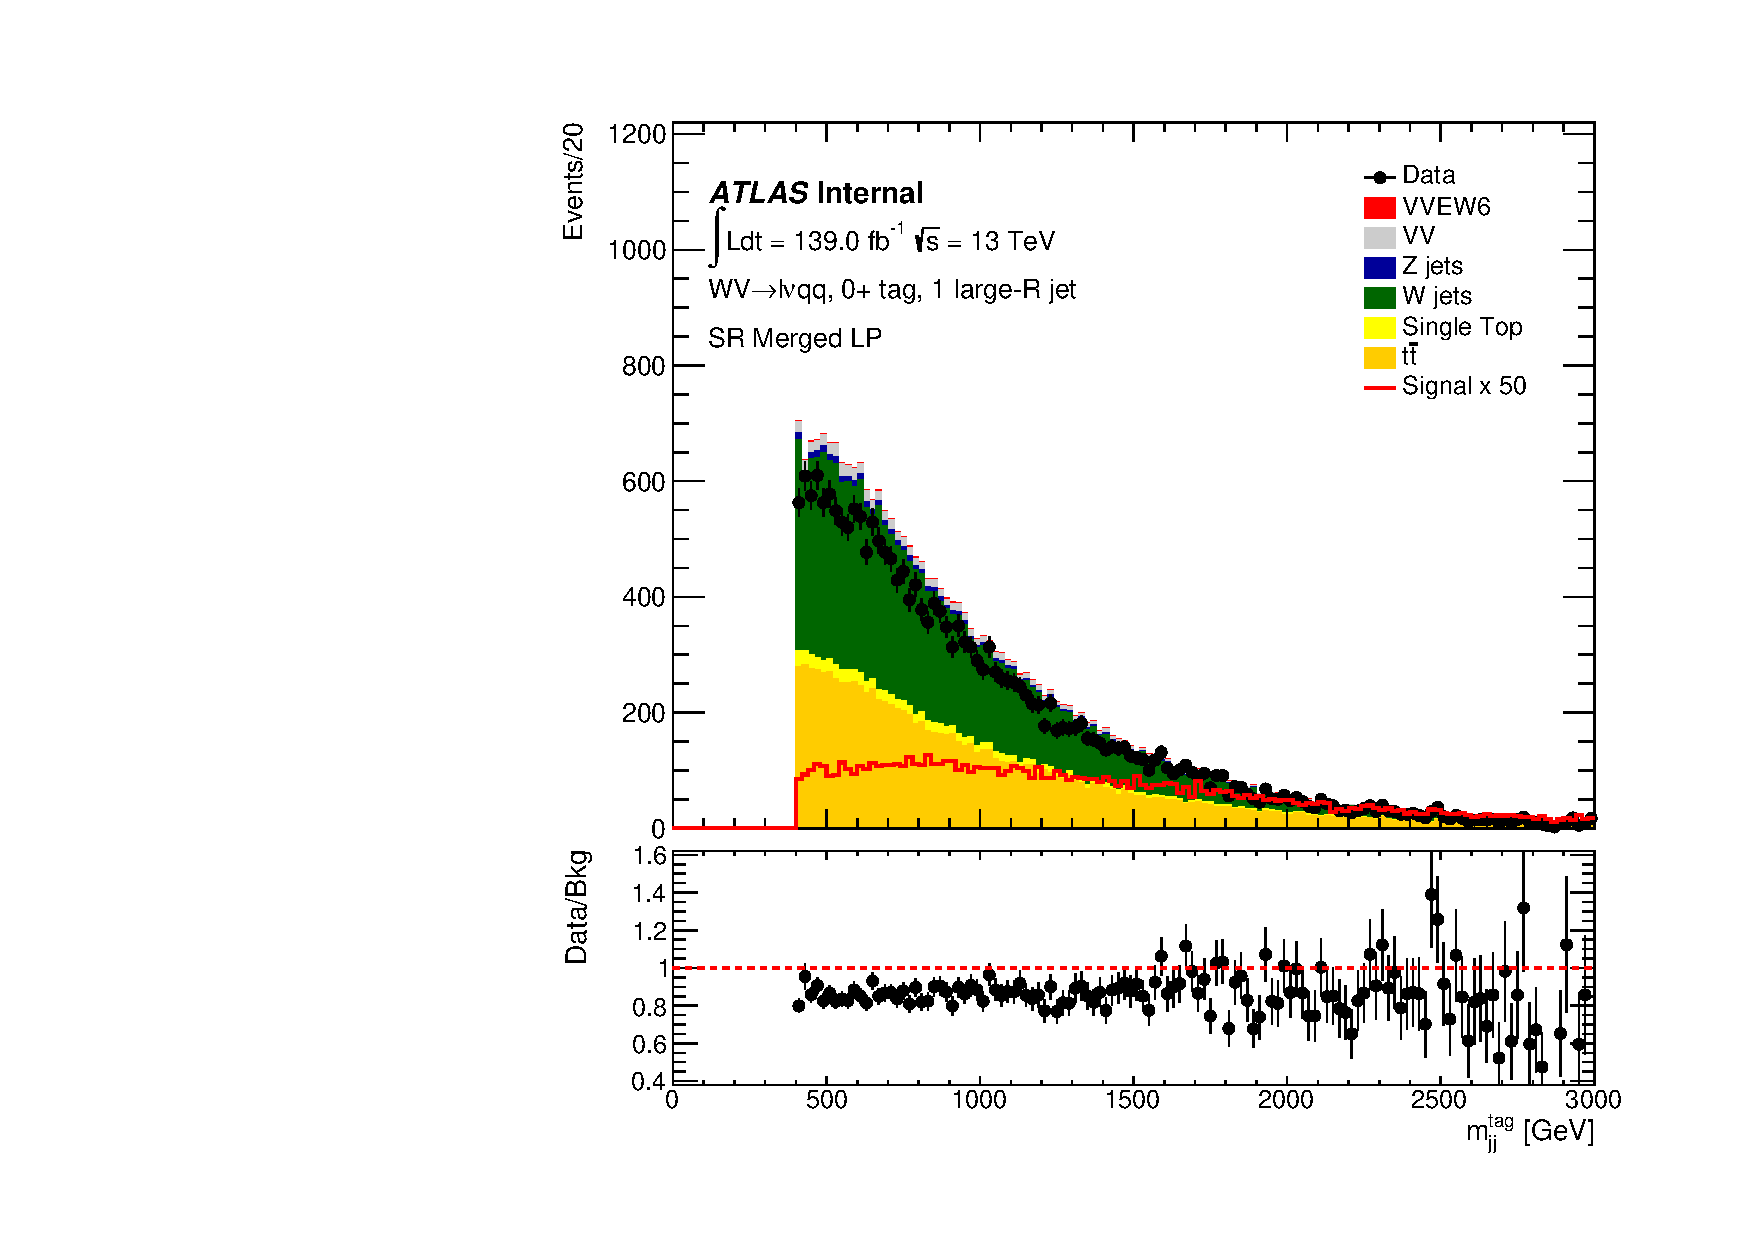
\includegraphics[width=\textwidth]{figures/mjjreweight1lep/SR_80/stacked_plot_merged_tagMjj.pdf}
        \caption{Merged LP SR}
        \label{fig:MC16ADE_Merged_LP_SR}
    \end{subfigure}
    \hfill
    \begin{subfigure}[b]{0.3\textwidth}
        \centering
        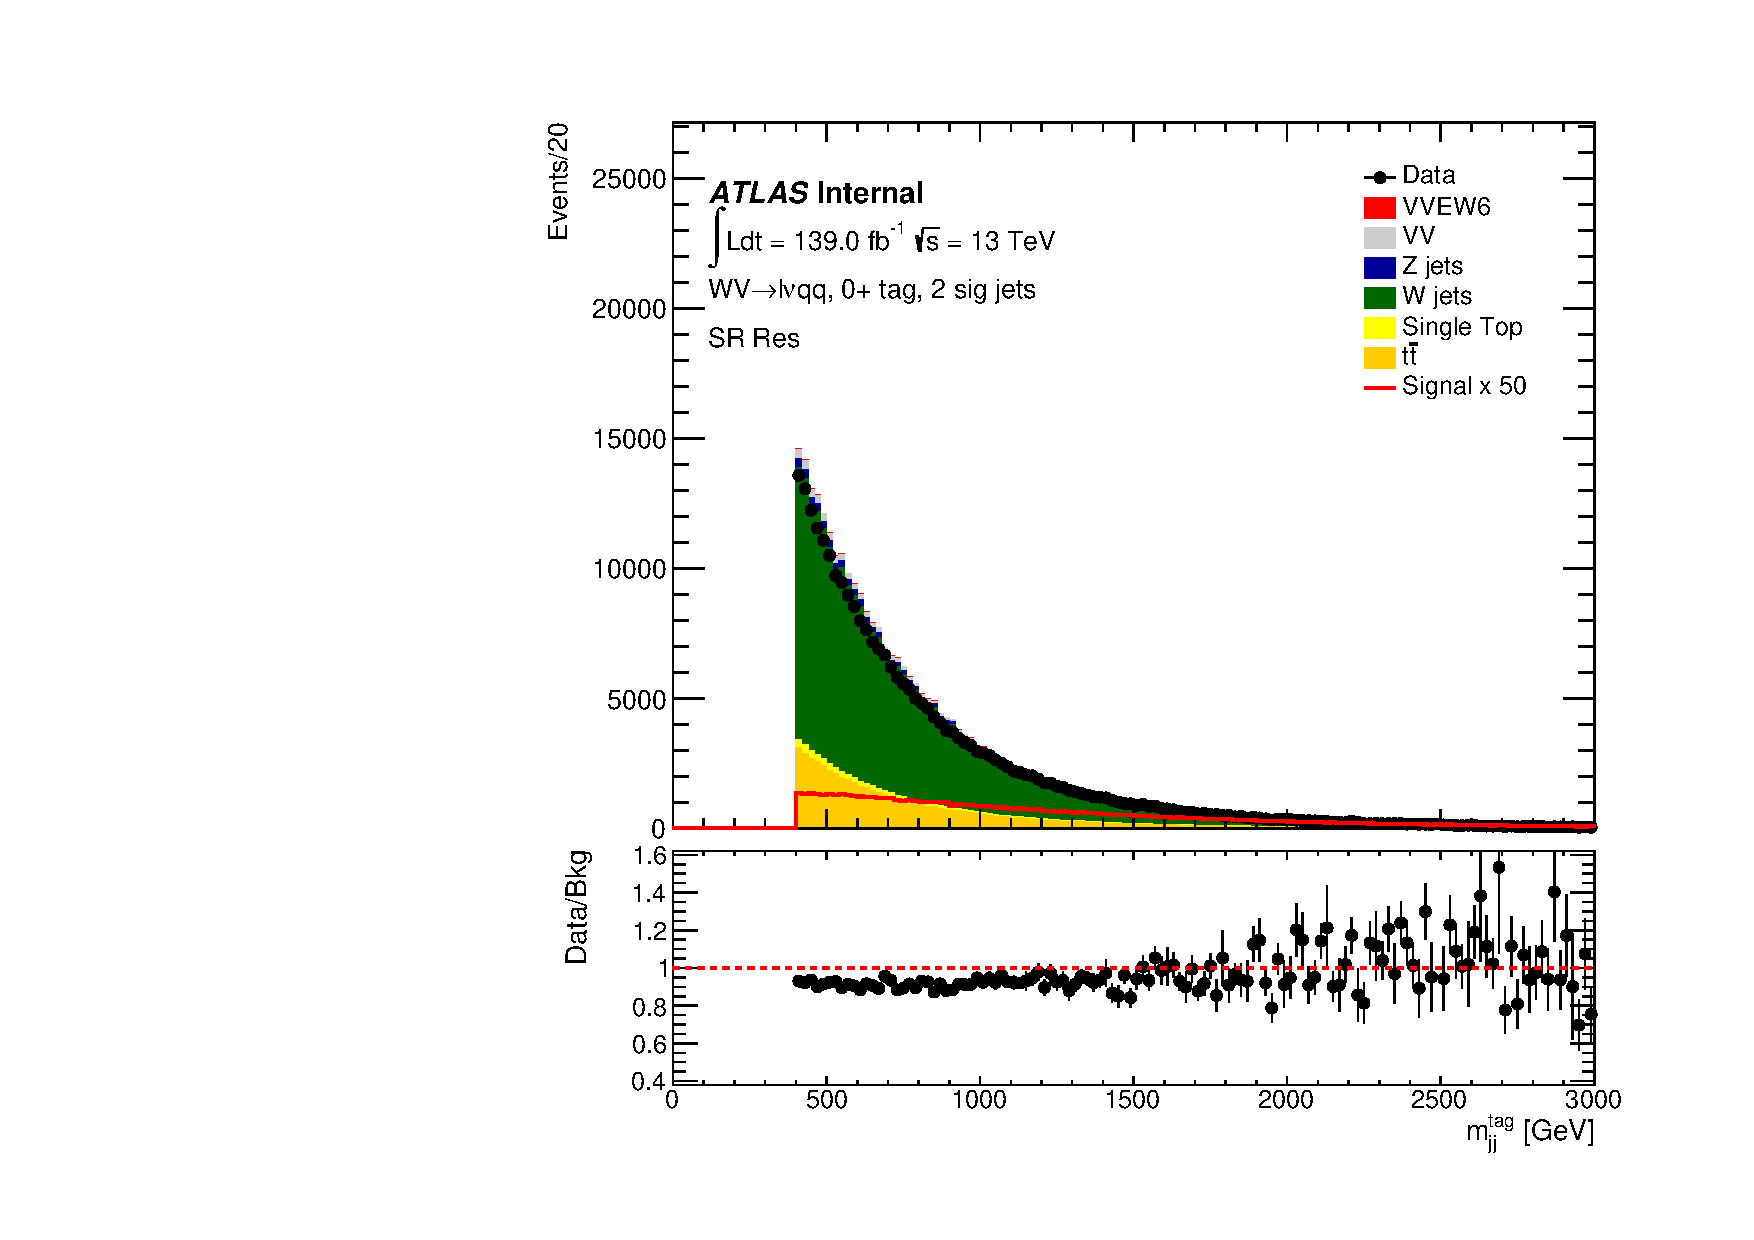
\includegraphics[width=\textwidth]{figures/mjjreweight1lep/SR_Res/stacked_plot_resolved_tagMjj.pdf}
        \caption{Resolved SR}
        \label{fig:MC16ADE_Resolved_SR}
    \end{subfigure}
    \caption{\(\mjjtag\) distributions after applying mjj-reweighting in the signal regions.}
    \label{fig:mjjReweight1LepMjjDistAfter}
\end{figure}

%%%\begin{figure}[ht]
%%%    \centering
%%%    \begin{subfigure}{0.7\textwidth}
%%%        \centering
%%%        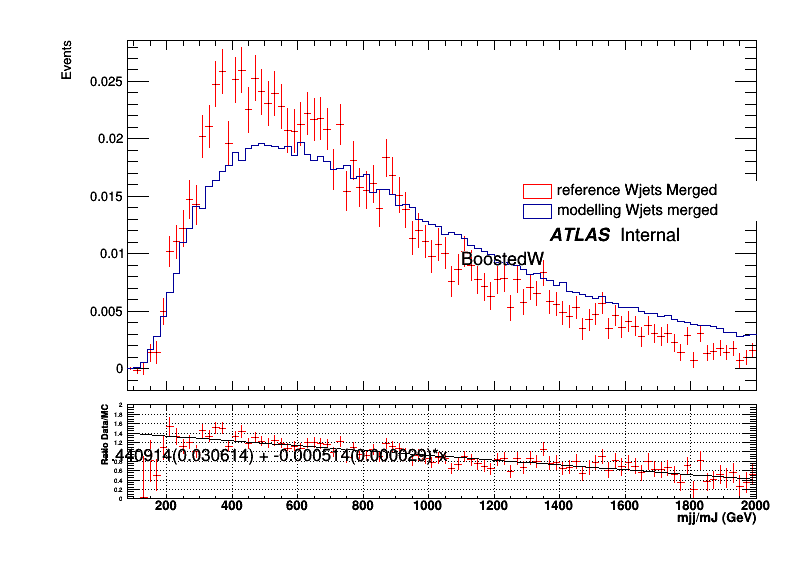
\includegraphics[width=\textwidth]{figures/mjjreweight1lep/merged_WjetsAllMC16T.png}
%%%        \caption{Fit of \(\mjjtag\) slope in merged region, for the entire \(M_J\) range.}
%%%        \label{fig:mjjReweight1LepMer}
%%%    \end{subfigure}
%%%\end{figure}

\begin{figure}[ht]
    \centering
    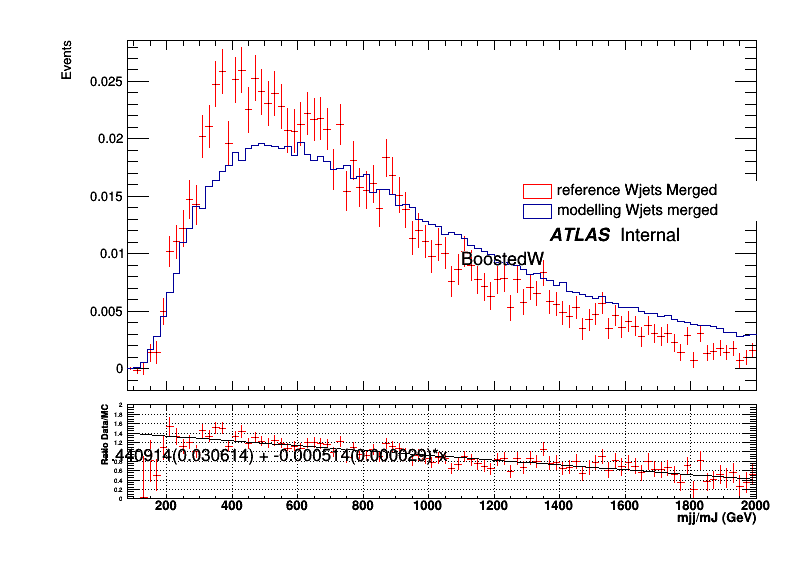
\includegraphics[width=0.7\textwidth]{figures/mjjreweight1lep/merged_WjetsAllMC16T.png}
    \caption{Fit of \(\mjjtag\) slope across the full \(M_J\) range in the merged region.}
    \label{fig:mjjReweight1LepMer}
\end{figure}

\begin{figure}[ht]
    \centering
    \begin{subfigure}[b]{0.3\textwidth}
        \centering
        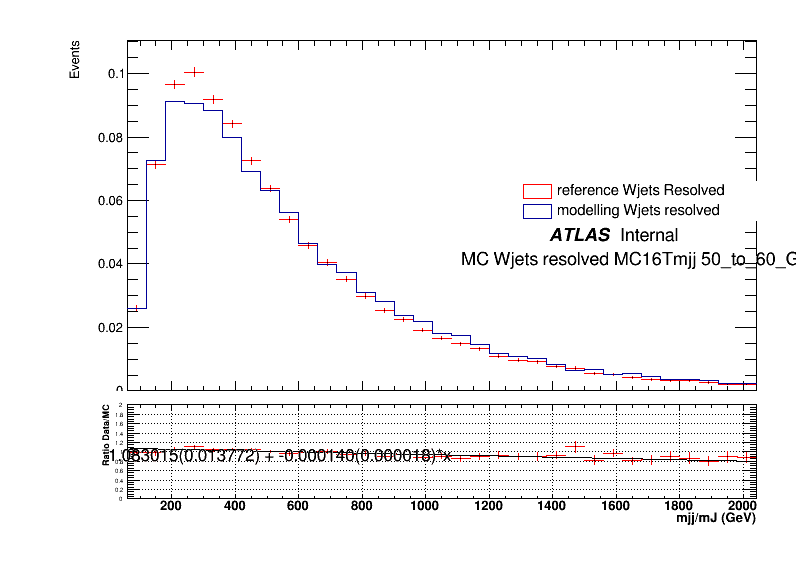
\includegraphics[width=\textwidth]{figures/mjjreweight1lep/resolved_Wjets50_to_60_GeVMC16T.png}
        \caption{50GeV to 60GeV bin}
        \label{fig:resolved_Wjets50to60}
    \end{subfigure}
    \hfill % This will add spacing between the subfigures if needed
    \begin{subfigure}[b]{0.3\textwidth}
        \centering
        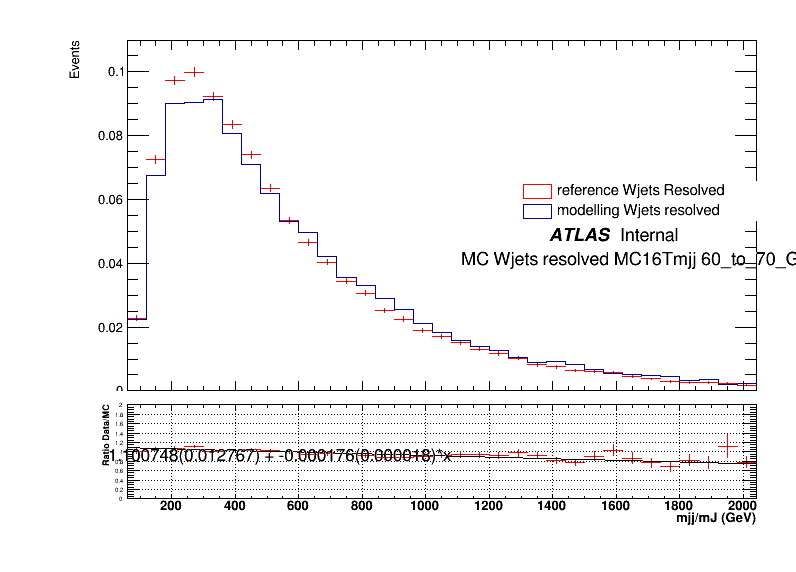
\includegraphics[width=\textwidth]{figures/mjjreweight1lep/resolved_Wjets60_to_70_GeVMC16T.png}
        \caption{60GeV to 70GeV bin}
        \label{fig:resolved_Wjets60to70}
    \end{subfigure}
    \hfill
    \begin{subfigure}[b]{0.3\textwidth}
        \centering
        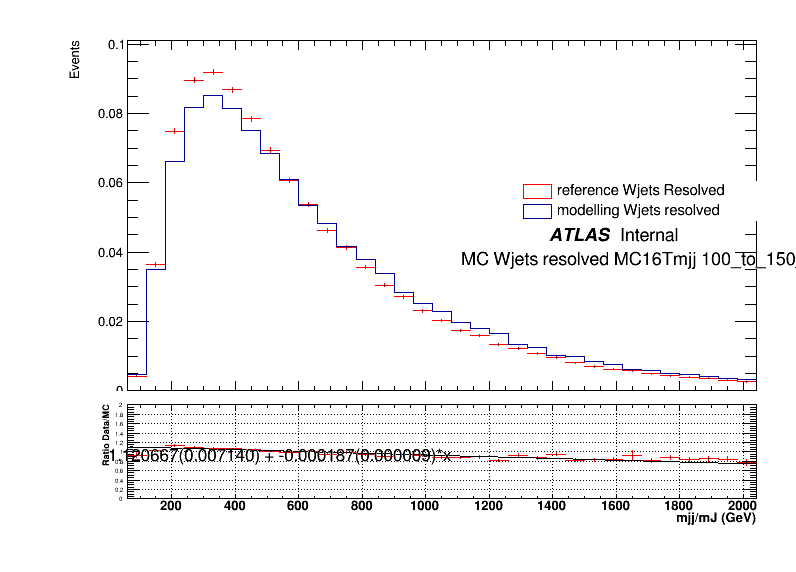
\includegraphics[width=\textwidth]{figures/mjjreweight1lep/resolved_Wjets100_to_150_GeVMC16T.png}
        \caption{100GeV to 150GeV bin}
        \label{fig:resolved_Wjets100to150}
    \end{subfigure}
    % Note: If you want the next subfigures to be on the next line, add a \par or simply remove the \hfill commands above
    
    \begin{subfigure}[b]{0.3\textwidth}
        \centering
        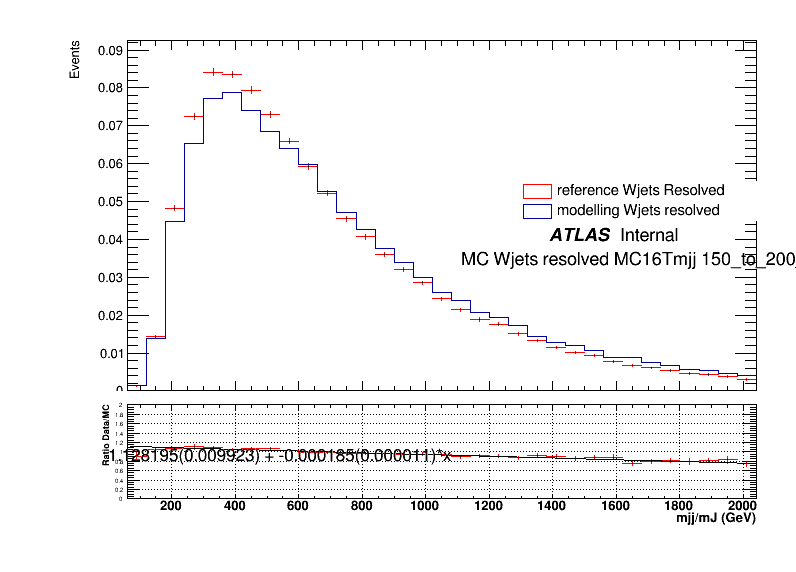
\includegraphics[width=\textwidth]{figures/mjjreweight1lep/resolved_Wjets150_to_200_GeVMC16T.png}
        \caption{150GeV to 200GeV bin}
        \label{fig:resolved_Wjets150to200}
    \end{subfigure}
%    \hfill
    \begin{subfigure}[b]{0.3\textwidth}
        \centering
        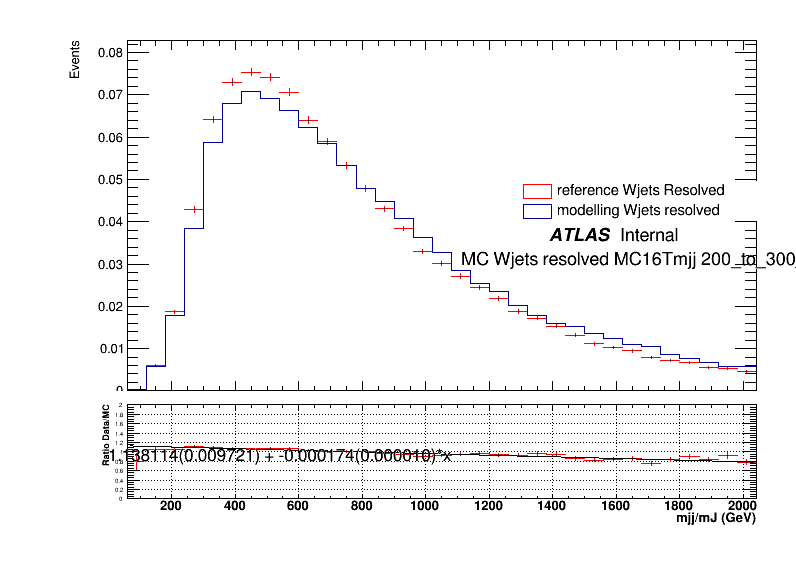
\includegraphics[width=\textwidth]{figures/mjjreweight1lep/resolved_Wjets200_to_300_GeVMC16T.png}
        \caption{200GeV to 300GeV bin}
        \label{fig:resolved_Wjets200to300}
    \end{subfigure}
    \caption{Fit of \(\mjjtag\) slope across various \(m_{jj}^{sig}\) slices in W+jet resolved control regions.}
    \label{fig:mjjReweight1LepResPtBins}
\end{figure}

\begin{figure}[ht]
    \centering
    \begin{subfigure}[b]{0.45\textwidth}
        \centering
        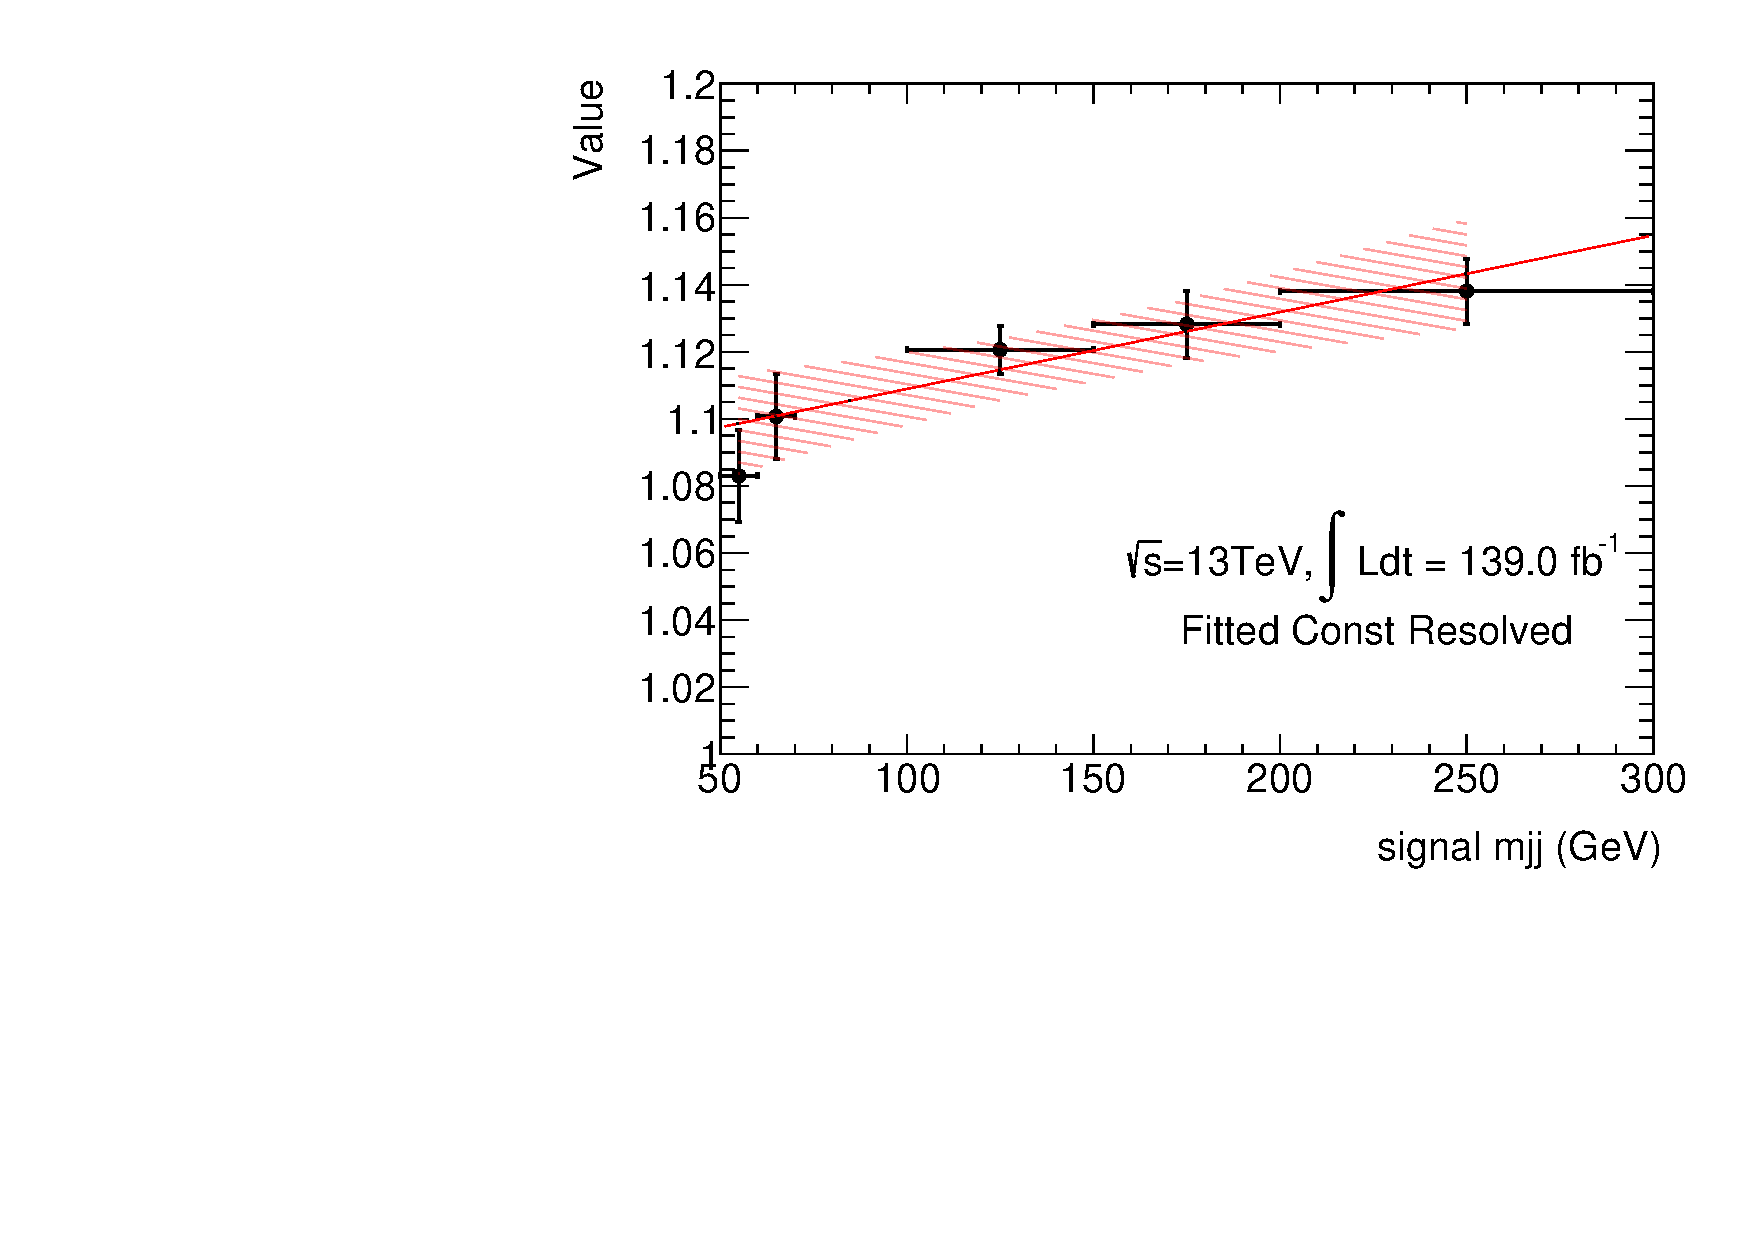
\includegraphics[width=\textwidth]{figures/mjjreweight1lep/fitCResMC16T.pdf}
        \caption{Fit results for ``Constant'', $p_0$.}
        \label{fig:fitCRes}
    \end{subfigure}
    \hfill
    \begin{subfigure}[b]{0.45\textwidth}
        \centering
        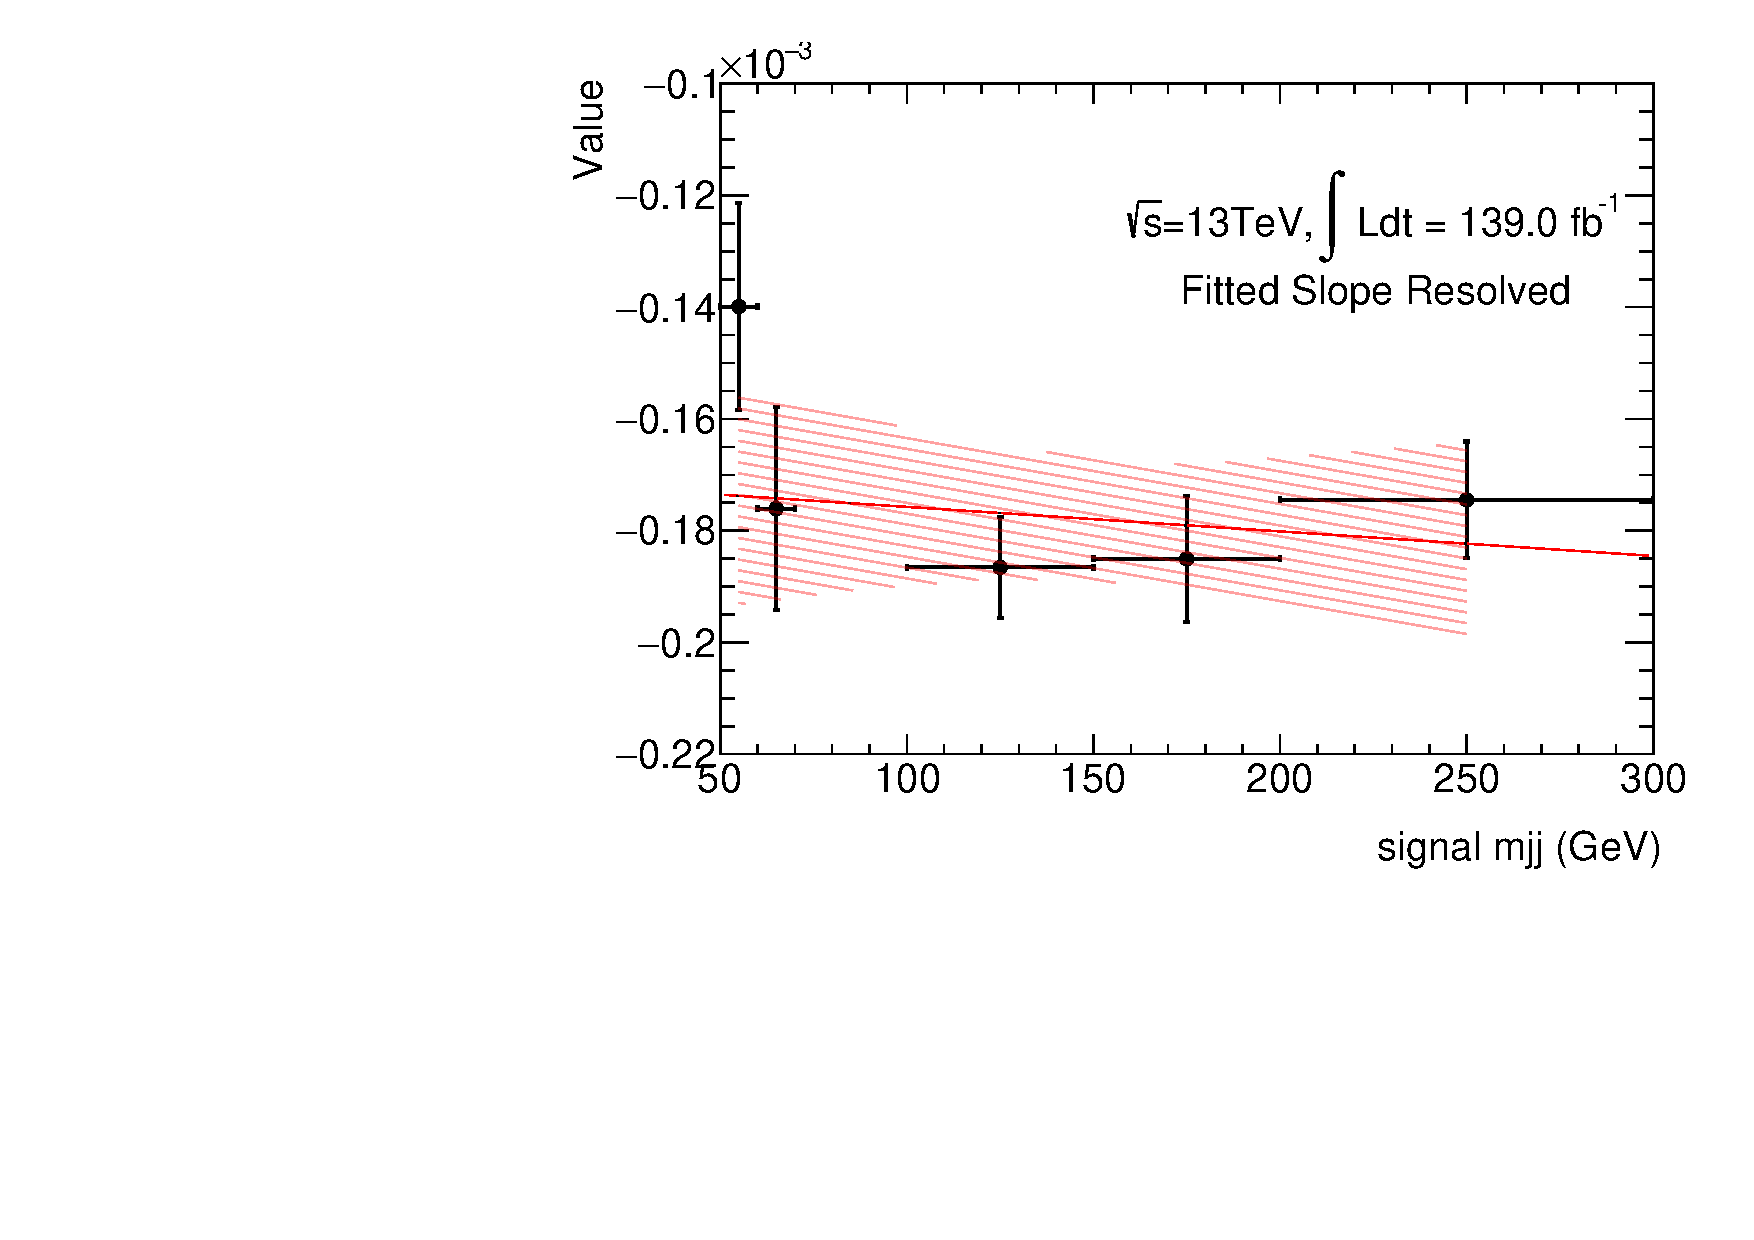
\includegraphics[width=\textwidth]{figures/mjjreweight1lep/fitSResMC16T.pdf}
        \caption{Fit results for ``Slope'', $p_1$.}
        \label{fig:fitSRes}
    \end{subfigure}
    \caption{Slopes and constants as a function of \(m_{jj}^{sig}\), with the red band indicating the 68\% confidence level of the fit. The fitted linear function is shown at the top and the fitted result at the signal \(m_{jj}^{sig}\) bin is shown at the bottom.}
    \label{fig:mjjReweight1LepResFit}
\end{figure}

\begin{figure}[ht]
    \centering
    \begin{subfigure}[b]{0.45\textwidth}
        \centering
        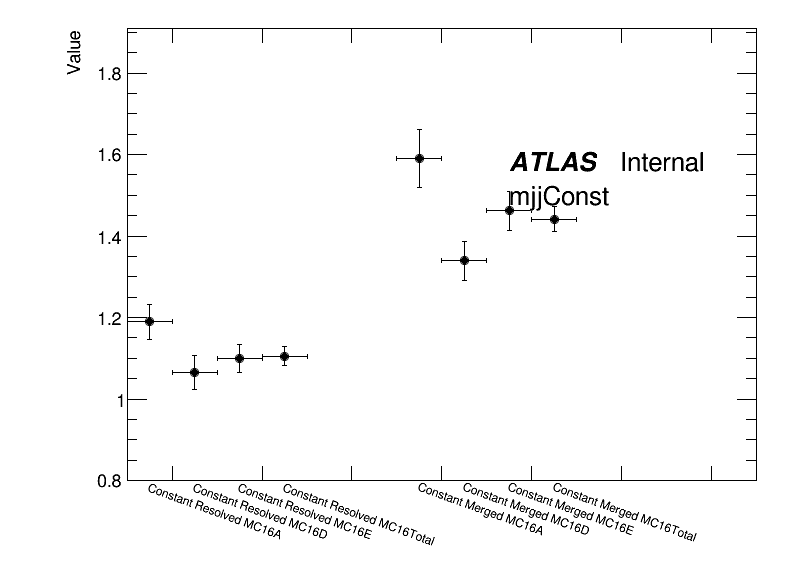
\includegraphics[width=\textwidth]{figures/mjjreweight1lep/TotalConstant.png}
        \caption{Fitted results for ``Constant'', $p_0$.}
        \label{fig:TotalConstant}
    \end{subfigure}
    \hfill
    \begin{subfigure}[b]{0.45\textwidth}
        \centering
        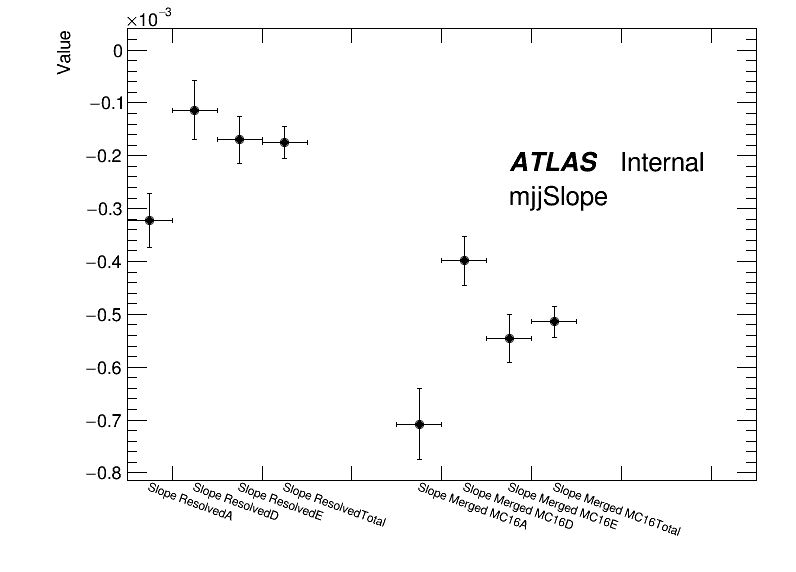
\includegraphics[width=\textwidth]{figures/mjjreweight1lep/TotalSlope.png}
        \caption{Fitted results for ``Slope'', $p_1$.}
        \label{fig:TotalSlope}
    \end{subfigure}
    \caption{Fitted results for slopes and constants for each data period.}
    \label{fig:mjjReweight1LepResTotal}
\end{figure}


%%\begin{figure}[ht]
%%    \centering
%%    \subfigure[]{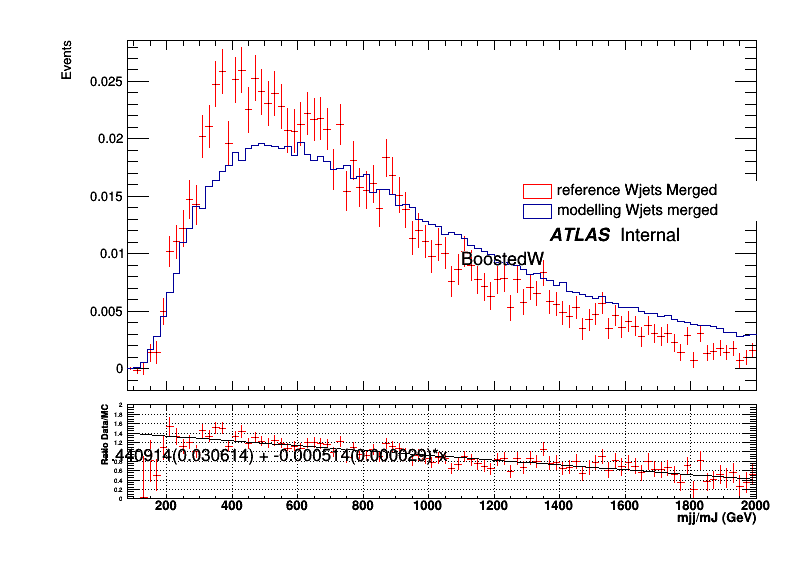
\includegraphics[width=0.7\textwidth]{figures/mjjreweight1lep/merged_WjetsAllMC16T.png}}
%%    \caption{Fit of \mjjtag slope in merged region, for the entire $M_J$ range. }
%%    \label{fig:mjjReweight1LepMer}
%%\end{figure}


%%%%%\begin{figure}[ht]
%%%%%    \centering
%%%%%    \subfigure[50GeV to 60GeV bin]{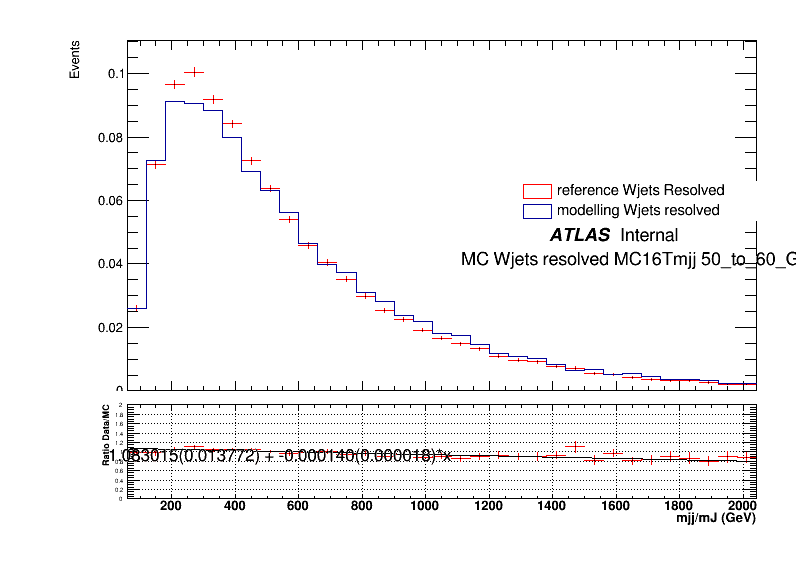
\includegraphics[width=0.3\textwidth]{figures/mjjreweight1lep/resolved_Wjets50_to_60_GeVMC16T.png}}
%%%%%    \subfigure[60GeV to 70GeV bin]{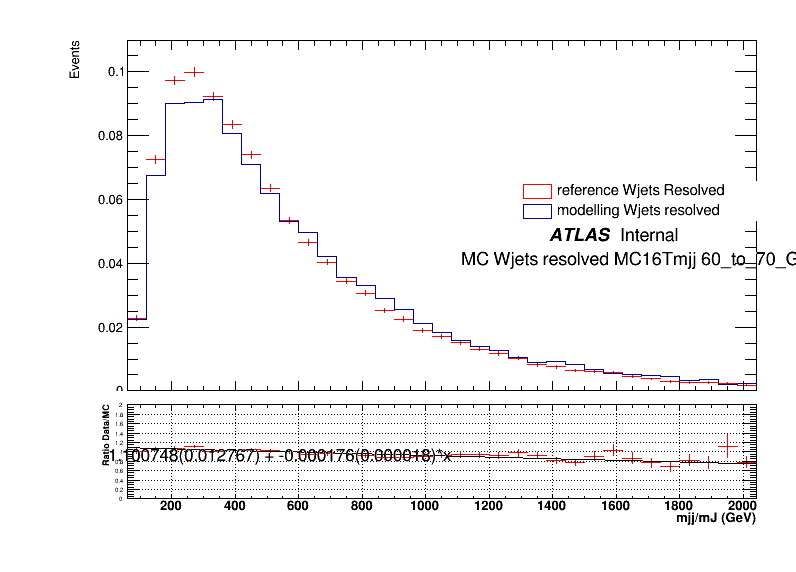
\includegraphics[width=0.3\textwidth]{figures/mjjreweight1lep/resolved_Wjets60_to_70_GeVMC16T.png}}
%%%%%    \subfigure[100GeV to 150GeV bin]{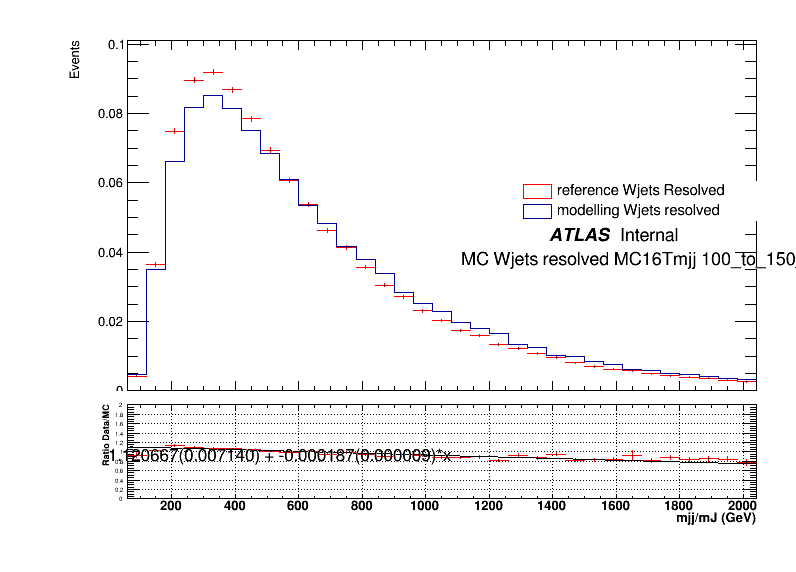
\includegraphics[width=0.3\textwidth]{figures/mjjreweight1lep/resolved_Wjets100_to_150_GeVMC16T.png}}
%%%%%    \subfigure[150GeV to 200GeV bin]{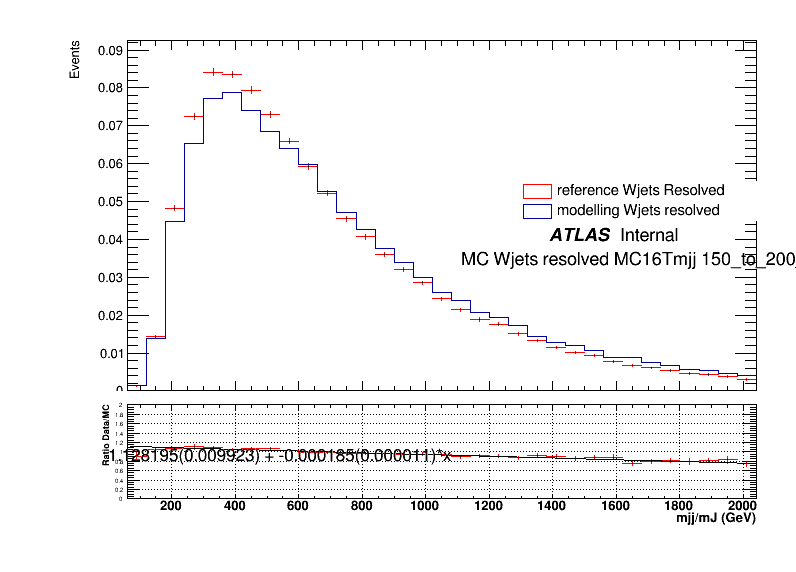
\includegraphics[width=0.3\textwidth]{figures/mjjreweight1lep/resolved_Wjets150_to_200_GeVMC16T.png}}
%%%%%    \subfigure[200GeV to 300GeV bin]{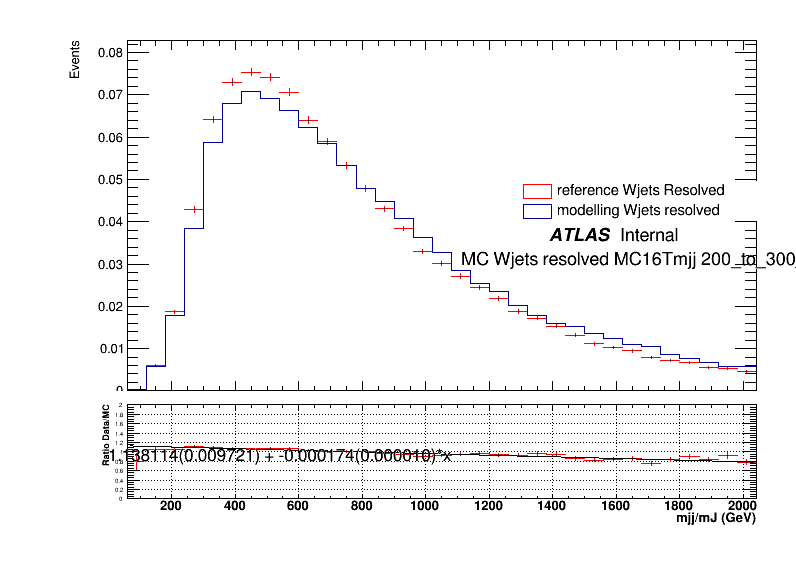
\includegraphics[width=0.3\textwidth]{figures/mjjreweight1lep/resolved_Wjets200_to_300_GeVMC16T.png}}
%%%%%    \caption{Fit of \mjjtag slope in W+jet resolved control regions, for different $m_{jj}^{sig}$ slices. }
%%%%%    \label{fig:mjjReweight1LepResPtBins}
%%%%%\end{figure}


%%%\begin{figure}[ht]
%%%    \centering
%%%    \subfigure[Fit results for "Constant".]{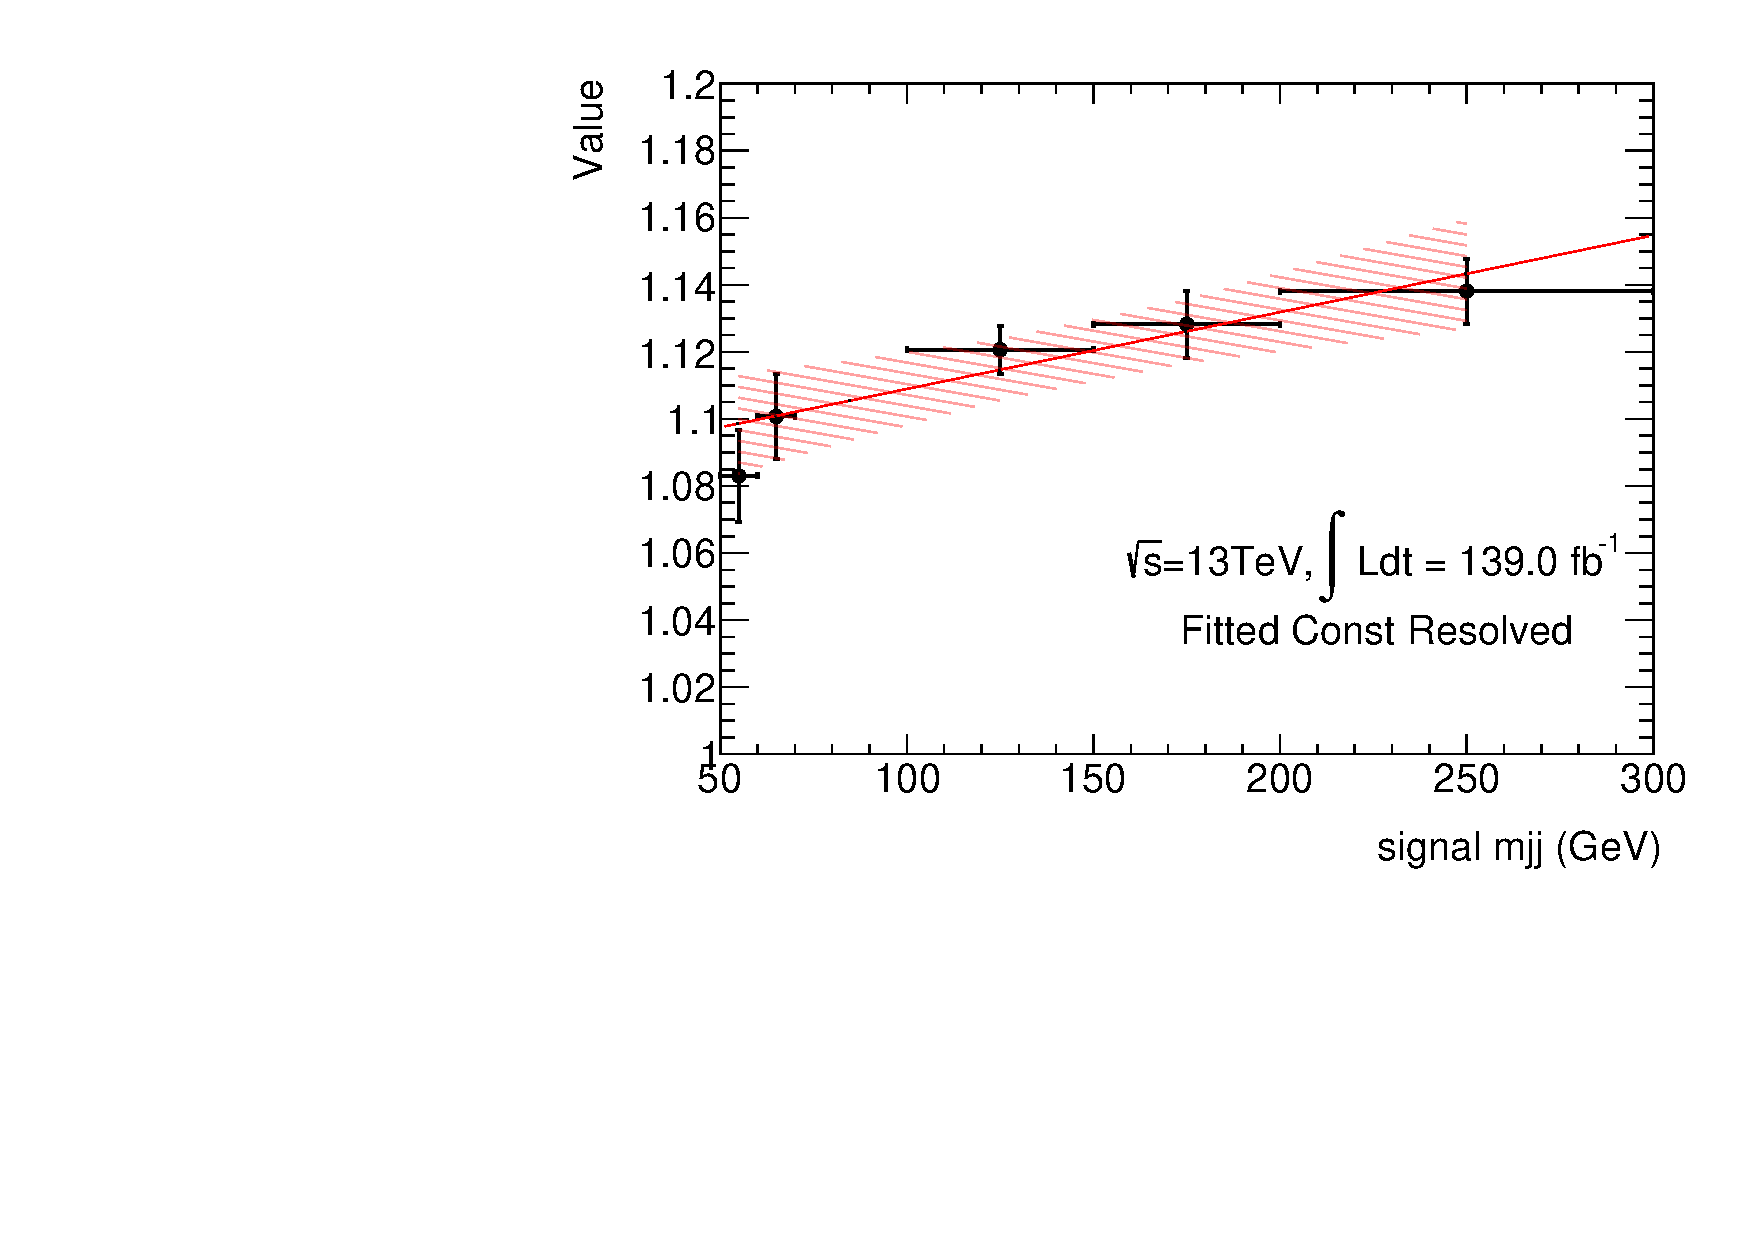
\includegraphics[width=0.45\textwidth]{figures/mjjreweight1lep/fitCResMC16T.pdf}}
%%%    \subfigure[Fit results for "Slope".]{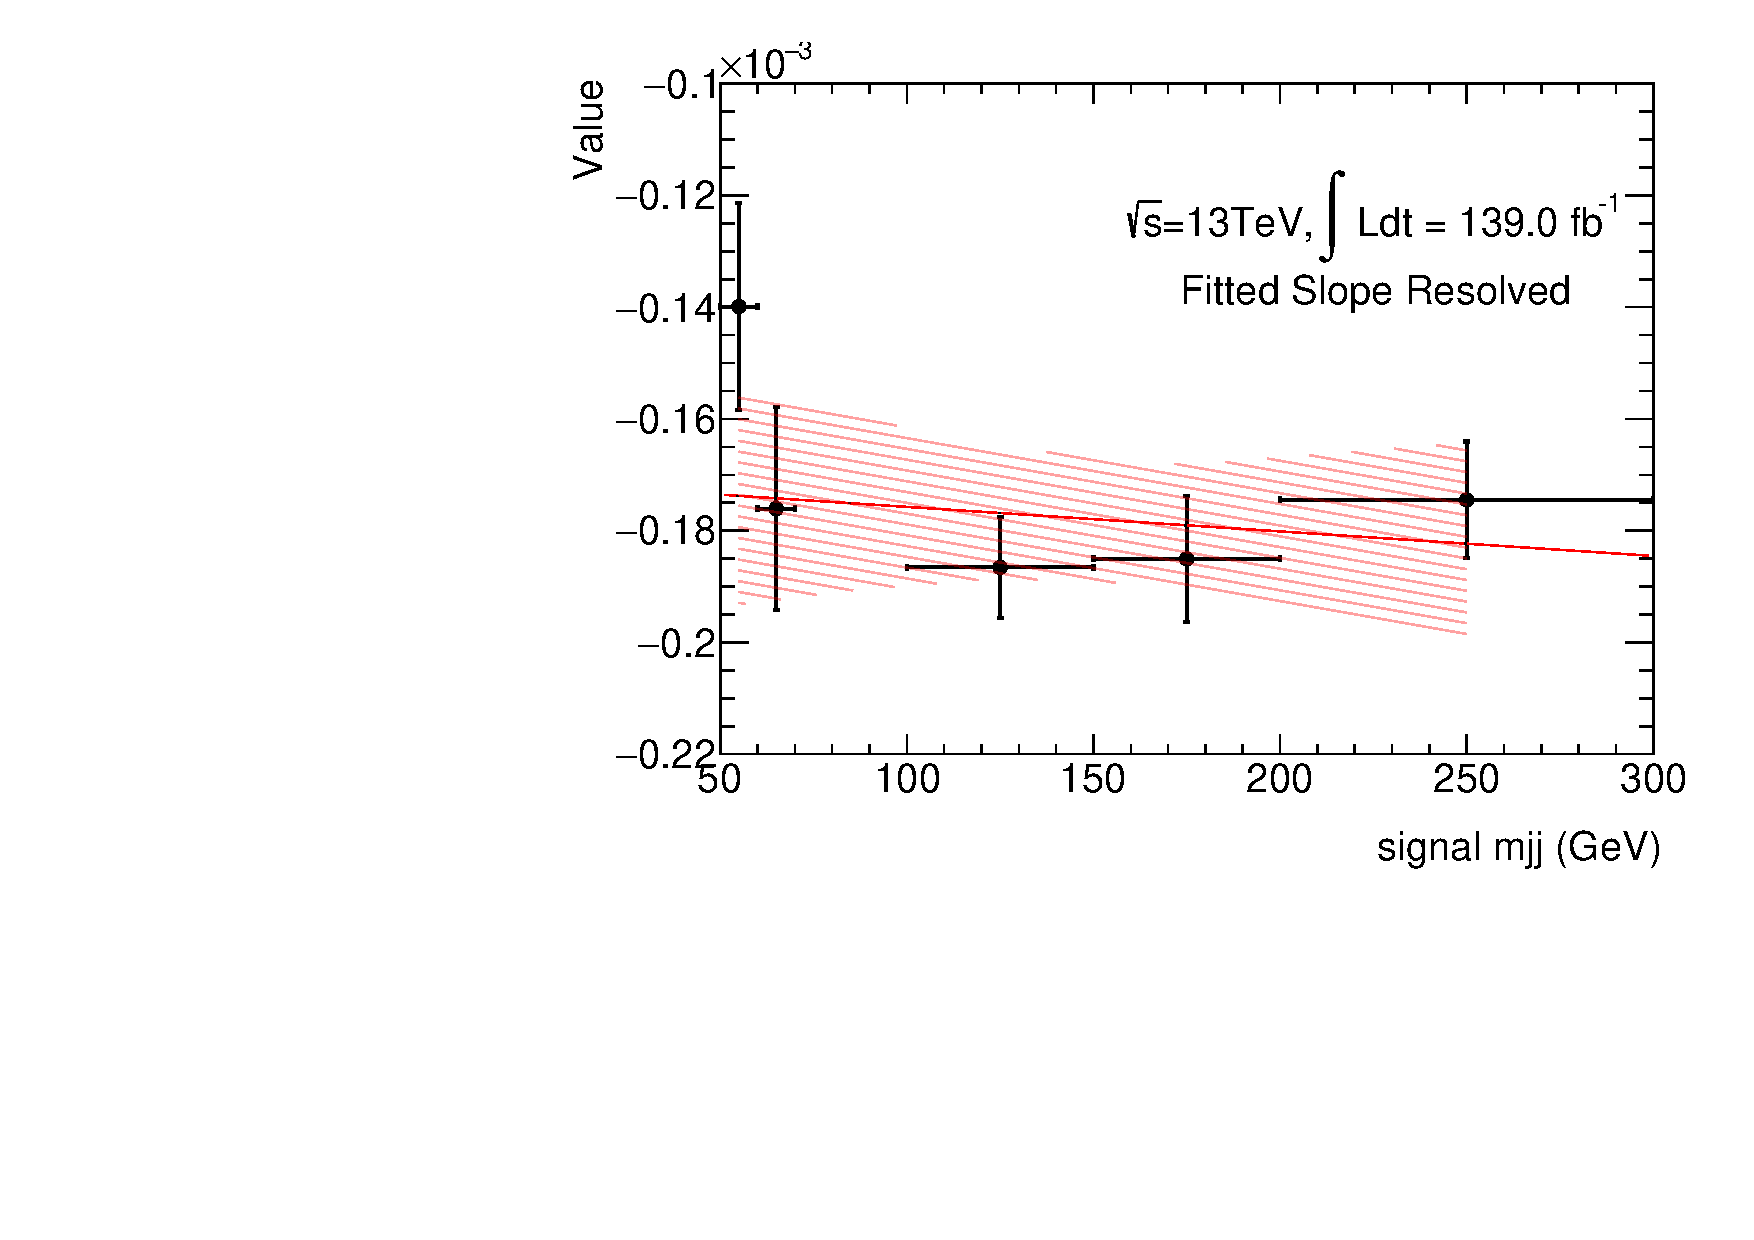
\includegraphics[width=0.45\textwidth]{figures/mjjreweight1lep/fitSResMC16T.pdf}}
%%%    \caption{Slopes and constants as a function of $m_{jj}^{sig}$. The red band presents the 68\% confidence level of the fit. The fitted linear function is shown at the top and the fitted result at the signal $m_{jj}^{sig}$ bin is shown at the bottom. }
%%%    \label{fig:mjjReweight1LepResFit}
%%%\end{figure}
%%%
%%%
%%%\begin{figure}[ht]
%%%    \centering
%%%    \subfigure[Fitted results for "Constant".]{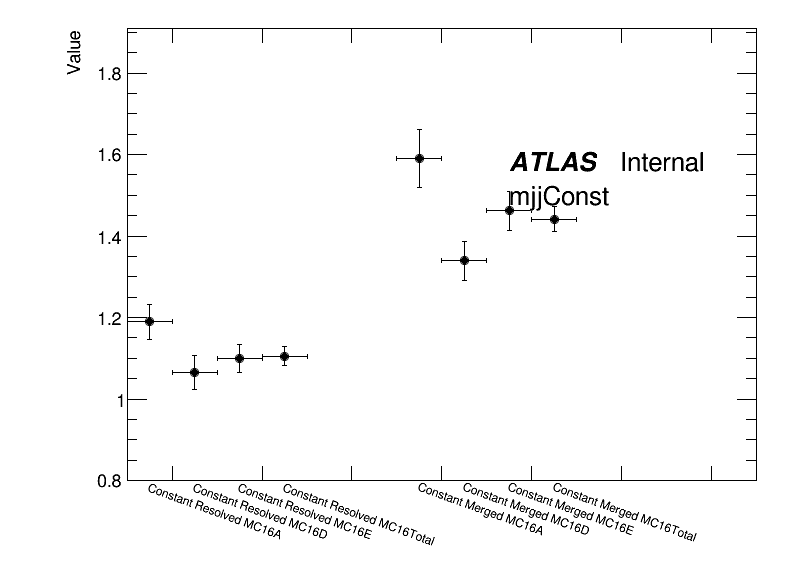
\includegraphics[width=0.45\textwidth]{figures/mjjreweight1lep/TotalConstant.png}}
%%%    \subfigure[Fitted results for "Slope".]{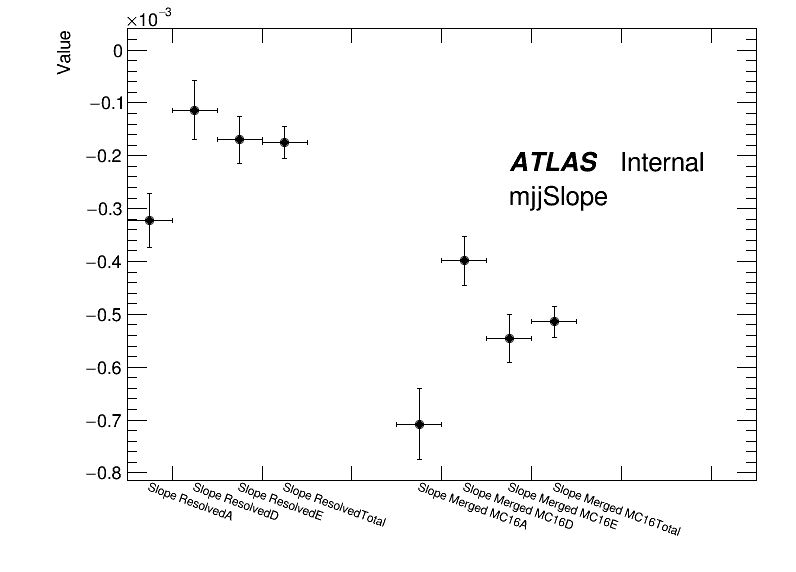
\includegraphics[width=0.45\textwidth]{figures/mjjreweight1lep/TotalSlope.png}}
%%%    \caption{Fitted results for slopes and constants for each data period.}
%%%    \label{fig:mjjReweight1LepResTotal}
%%%\end{figure}

%%%Table ~\ref{tab:1lepReweighting} shows the final parameters derived for the \olep channel.
%%%
%%%\begin{table}[ht]
%%%     \centering
%%%     \caption{1-lepton $m(jj)^\text{tag}$ reweighting factors.}
%%%     \label{tab:1lepReweighting}
%%%         \begin{tabular}{ |c|c|c| }
%%%\hline
%%%Parameter & Merged CRVjet & Resolved CRVjet  \\
%%%\hline
%%%$p_{0}$ (slope) [$\GeV^{-1}$] & $(-51.4 \pm 2.9)10^{-5}$ &  $(-14.4 \pm 6.1)10^{-5}$ \\
%%% \hline
%%%$p_{1}$ (constant)  & $1.47 \pm 0.03$ & $1.13 \pm 0.02$ \\
%%%\hline
%%%         \end{tabular}
%%%\end{table}

%%%%%%%%%%%%%%%%%%%%%%%%%%%%%%
%%%Assuming that the mis-modelling depends linearly on \mjjtag, we use the following equation
%%%to re-weight \Wjets events in an attempt to correct for this mis-modelling:
%%%
%%%\begin{equation}
%%%  w(m_{jj}^{tag}) =  p_0 + p_1 * m_{jj}^{tag} ,
%%%\end{equation}
%%%%
%%%where $p_0$ and $p_1$
%%%are parameters to be derived separately for merged and resolved regions. Once the slope and constants in the correction function are derived separately for merged and resolved cases in the control regions as defined in Table \ref{tab:mjjReweight1LepRegions}, it is then assumed that the corrections apply to the corresponding signal region. 
%%%In both the resolved and merged cases, these two constants are derived by fitting the ratio of Sherpa \Wjets modelling and data with non \Wjets background subtracted. In the resolved case, to account for possible dependence of the slope and constant on $m_{jj}^{sig}$, the reweighting study is performed in $m_{jj}^{sig}$ bins of [50,60,70,100,120,150,200,300] GeV, and an interpolation from the control region to the signal region is performed. In the merged case, a fit to the entire $m_{J}$ range is performed to get better statistical significance on the result. The fit results are shown in Figure \ref{fig:mjjReweight1LepResPtBins}, \ref{fig:mjjReweight1LepMer}. Once the constants and slopes have been derived for different $m_{jj}^{sig}$ bins, they are fitted to get the final result in the signal $m_{jj}^{sig}$ bin, as shown in Figure \ref{fig:mjjReweight1LepResFit}. \\

%%%All the above studies were done with all of the data periods and corresponding MC campaigns (mc16a, mc16d, and mc16e) combined. To check that there are no significant differences between different data periods and pileup conditions, the studies were repeated for each mc campaign and the result is shown in Figure \ref{fig:mjjReweight1LepResTotal}.


%%%
\clearpage
\section{\( W \) + Jets Control Region}
%\clearpage
%\subsection{W+jets control region}

Figure
\ref{fig:CRWjetResLoosePlots1Lep}
\ref{fig:CRWjetResLoosePlots1Lep2}
\ref{fig:CRWjetResTightPlots1Lep}
\ref{fig:CRWjetResTightPlots1Lep2}
\ref{fig:CRWjetMerPlots1Lep}
\ref{fig:CRWjetMerPlots1Lep2}
show the main relevant kinematic variable distributions in the \Wjets CR in \olep channel, after \mjjtag reweighting has been applied.

\begin{figure}[ht]
    \centering
    \subfloat[]{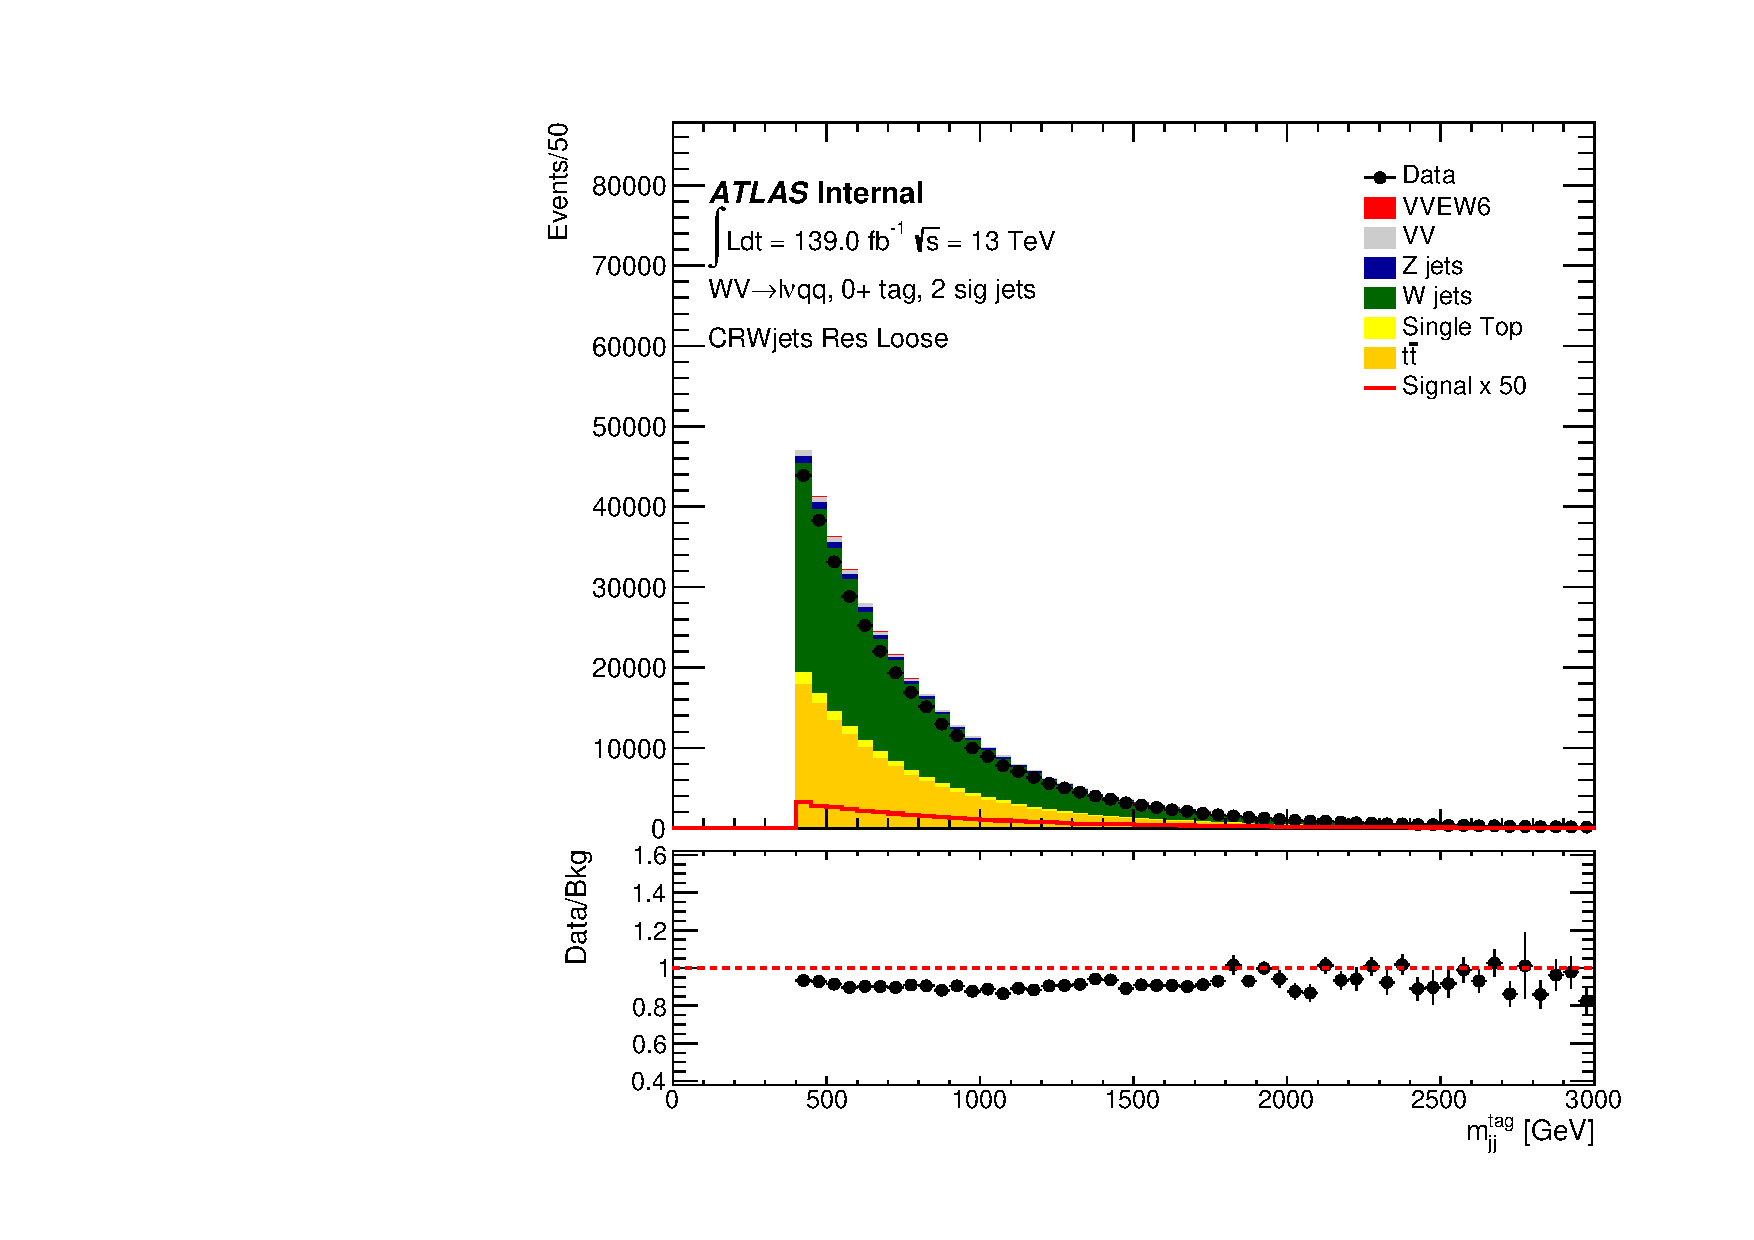
\includegraphics[width=0.3\textwidth]{figures/CRPlots/CRWjets_Res_Loose/stacked_plot_resolved_tagMjj.pdf}}
    \subfloat[]{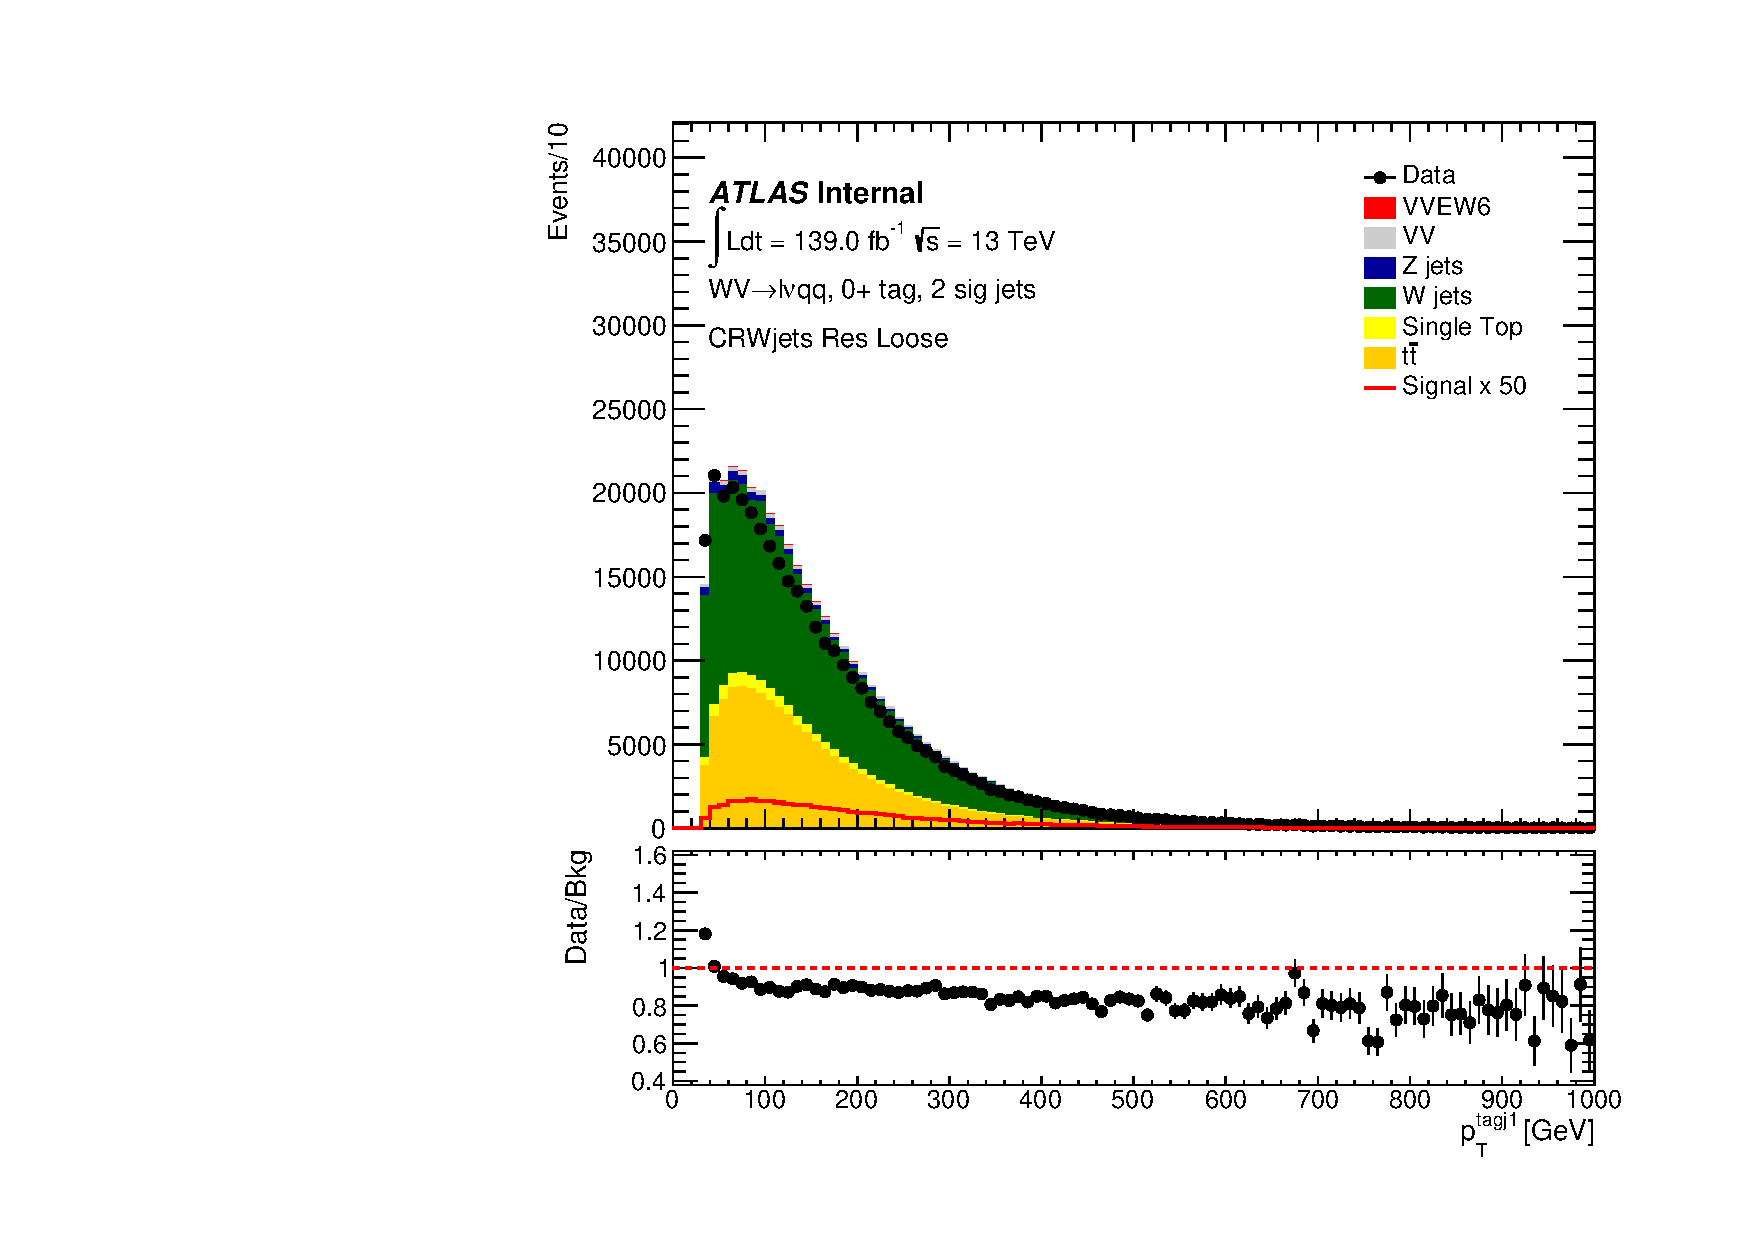
\includegraphics[width=0.3\textwidth]{figures/CRPlots/CRWjets_Res_Loose/stacked_plot_resolved_tagJ1_pt.pdf}}
    \subfloat[]{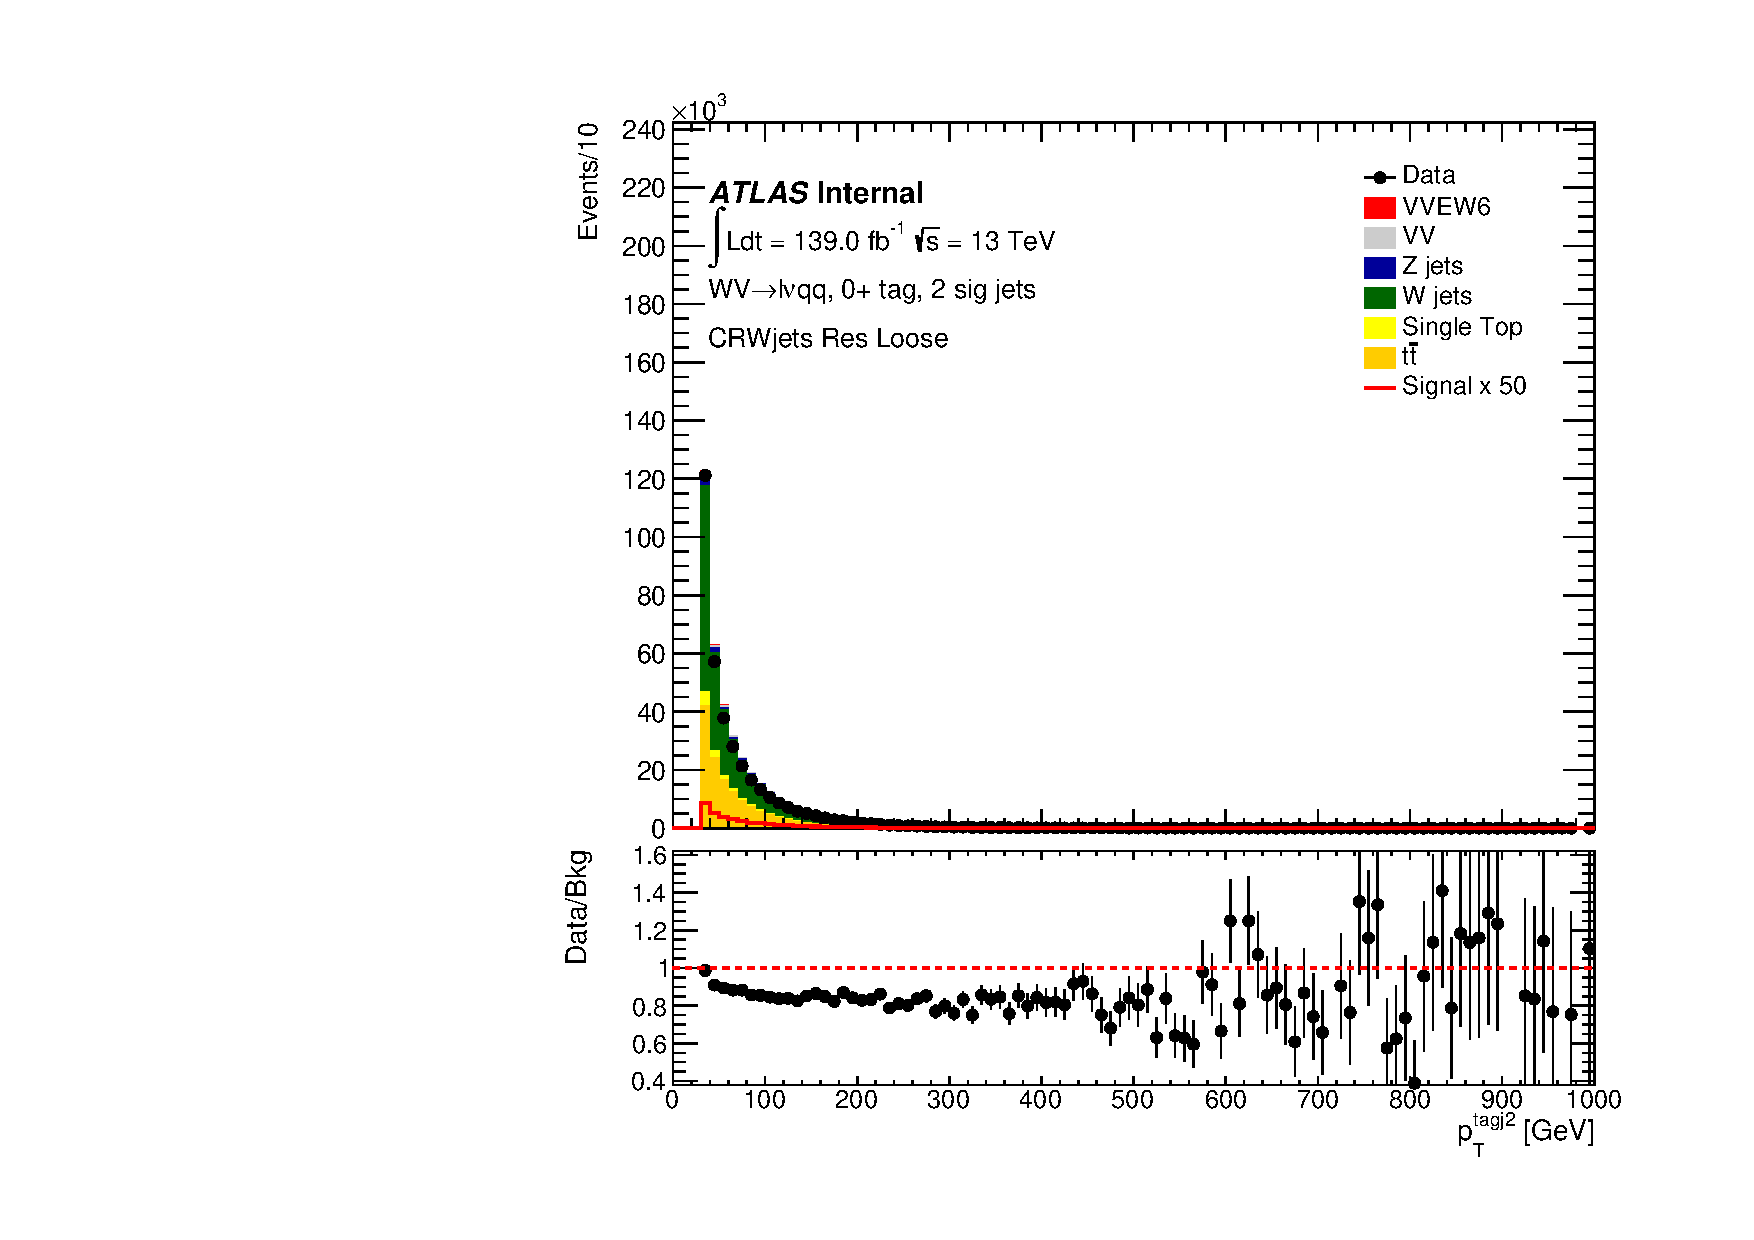
\includegraphics[width=0.3\textwidth]{figures/CRPlots/CRWjets_Res_Loose/stacked_plot_resolved_tagJ2_pt.pdf}} \\
    \subfloat[]{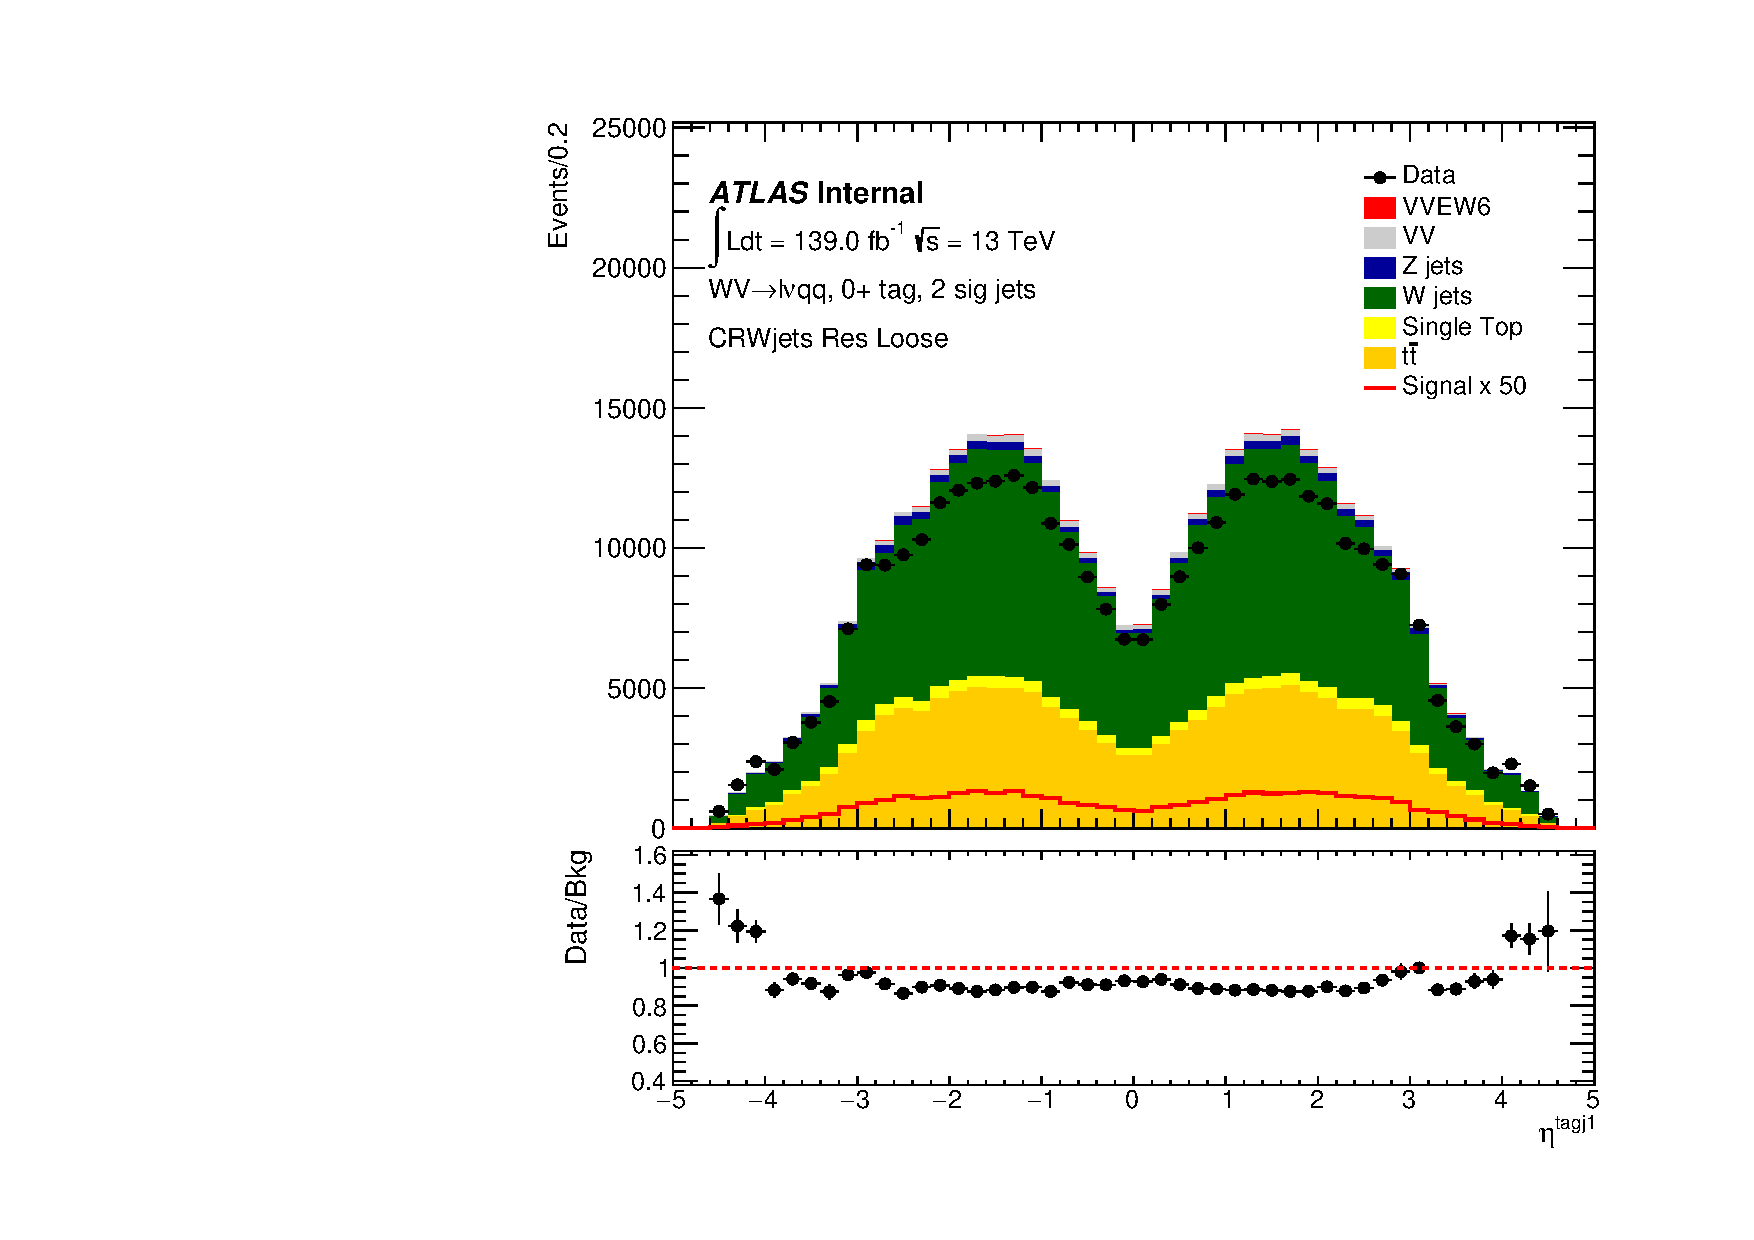
\includegraphics[width=0.3\textwidth]{figures/CRPlots/CRWjets_Res_Loose/stacked_plot_resolved_tagJ1_eta.pdf}}
    \subfloat[]{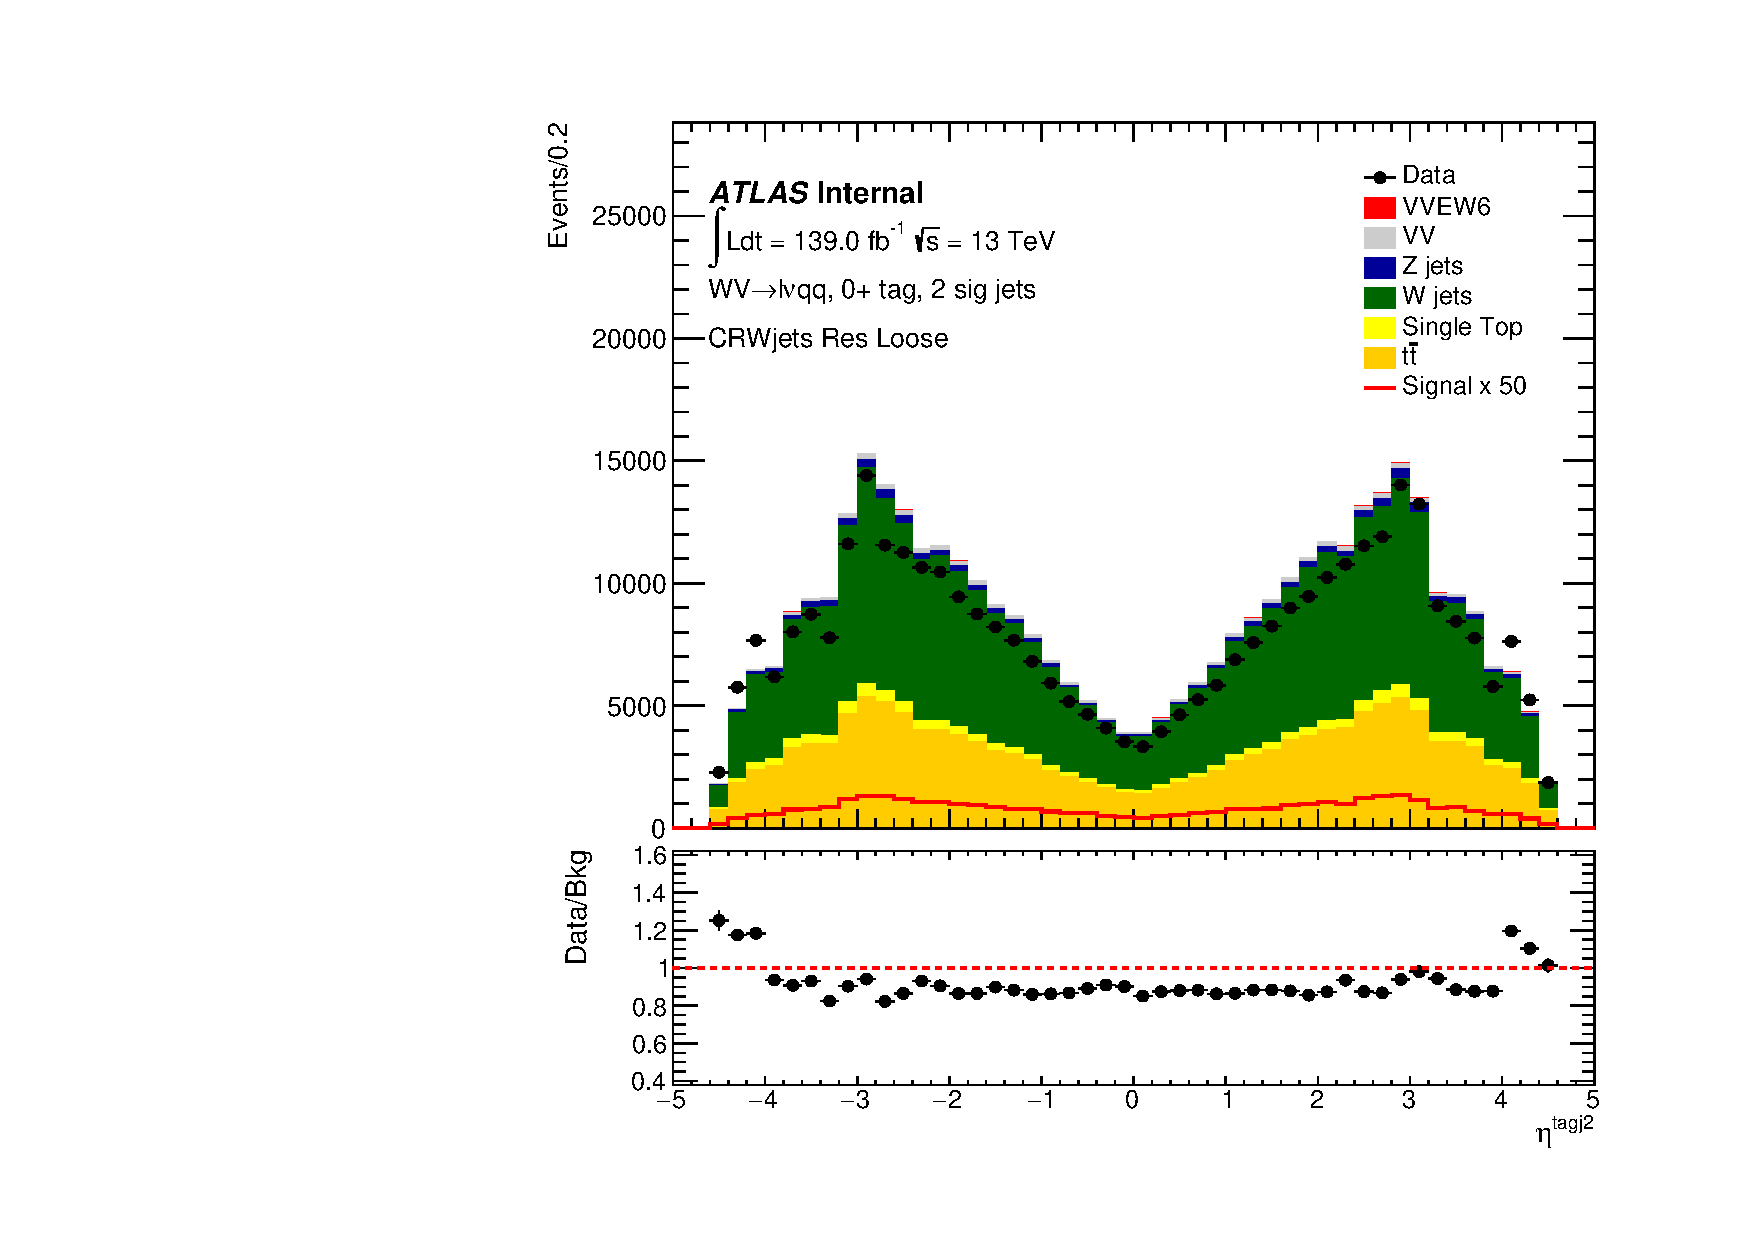
\includegraphics[width=0.3\textwidth]{figures/CRPlots/CRWjets_Res_Loose/stacked_plot_resolved_tagJ2_eta.pdf}} \\
    \subfloat[]{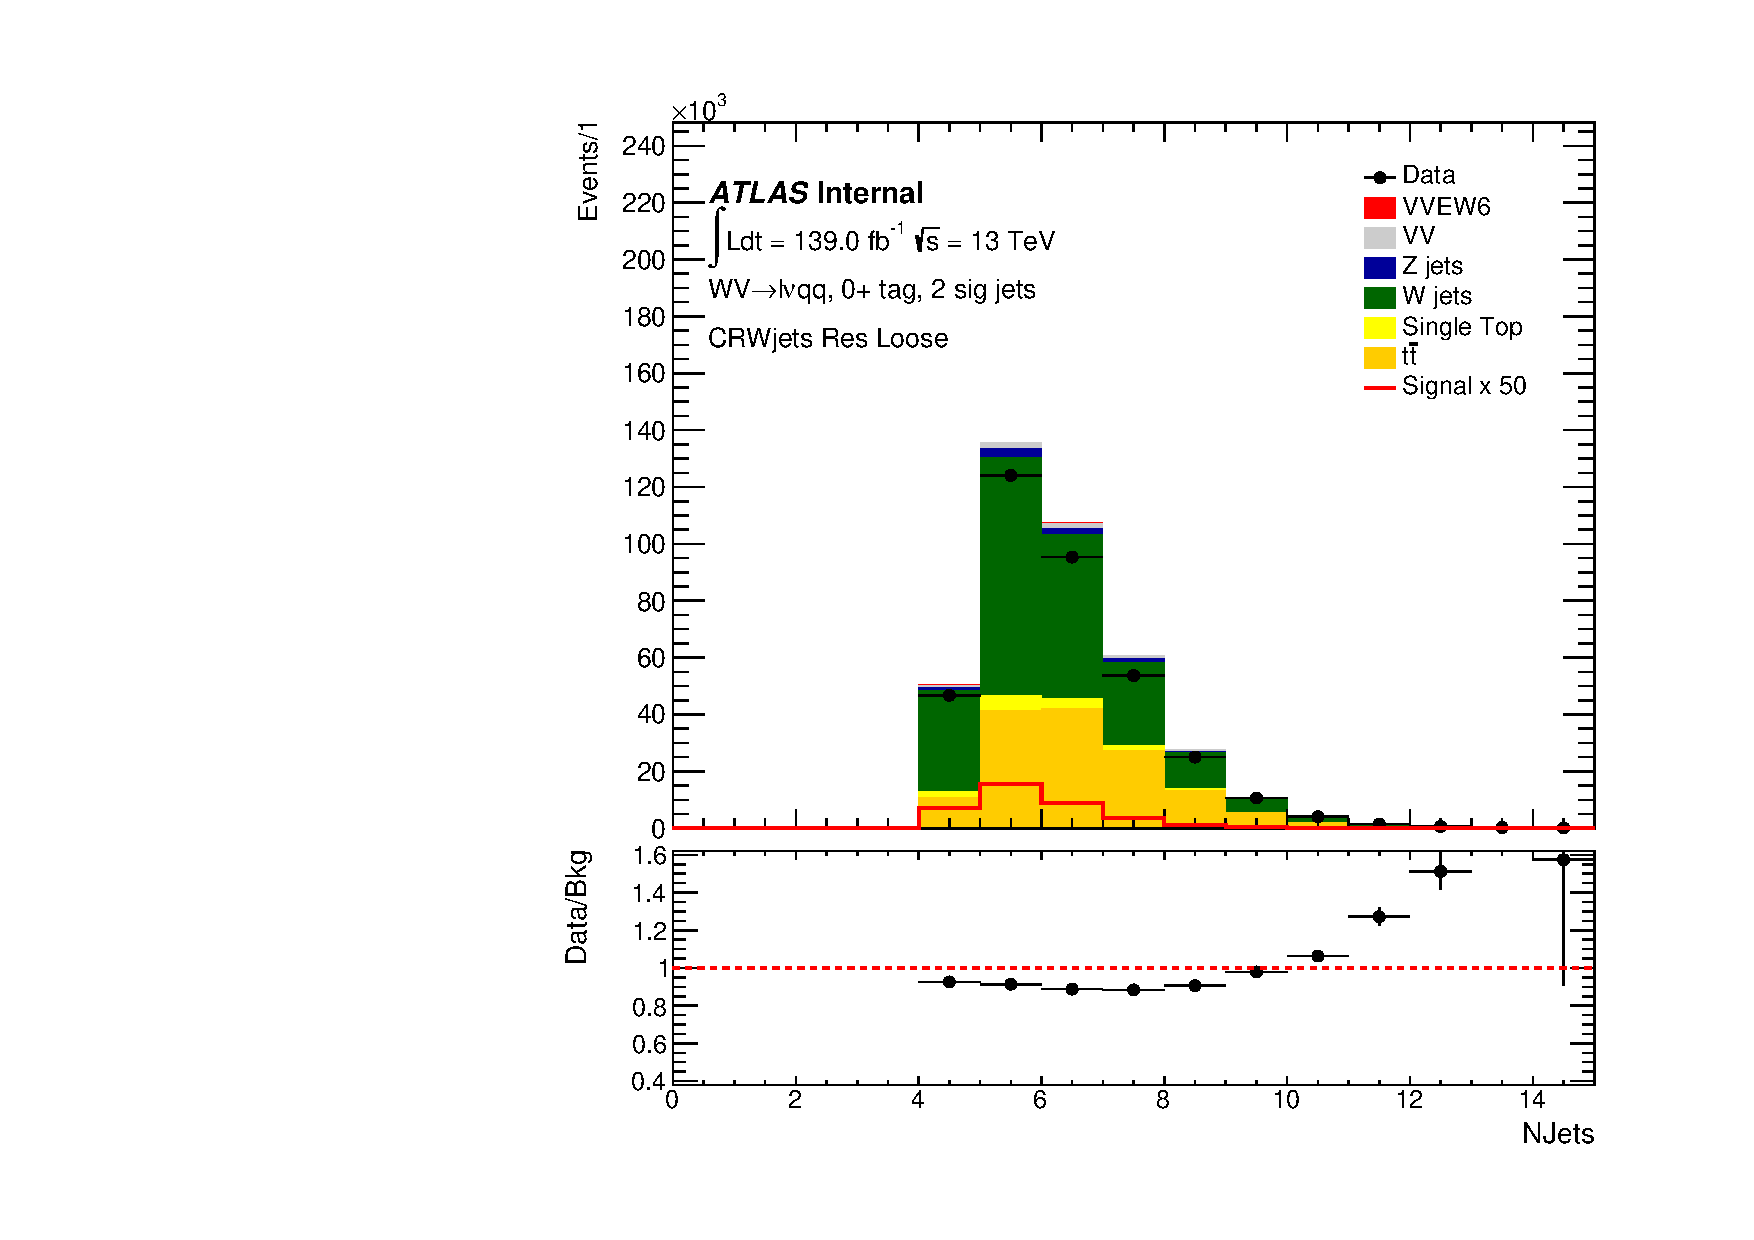
\includegraphics[width=0.3\textwidth]{figures/CRPlots/CRWjets_Res_Loose/stacked_plot_NJets.pdf}}
    \subfloat[]{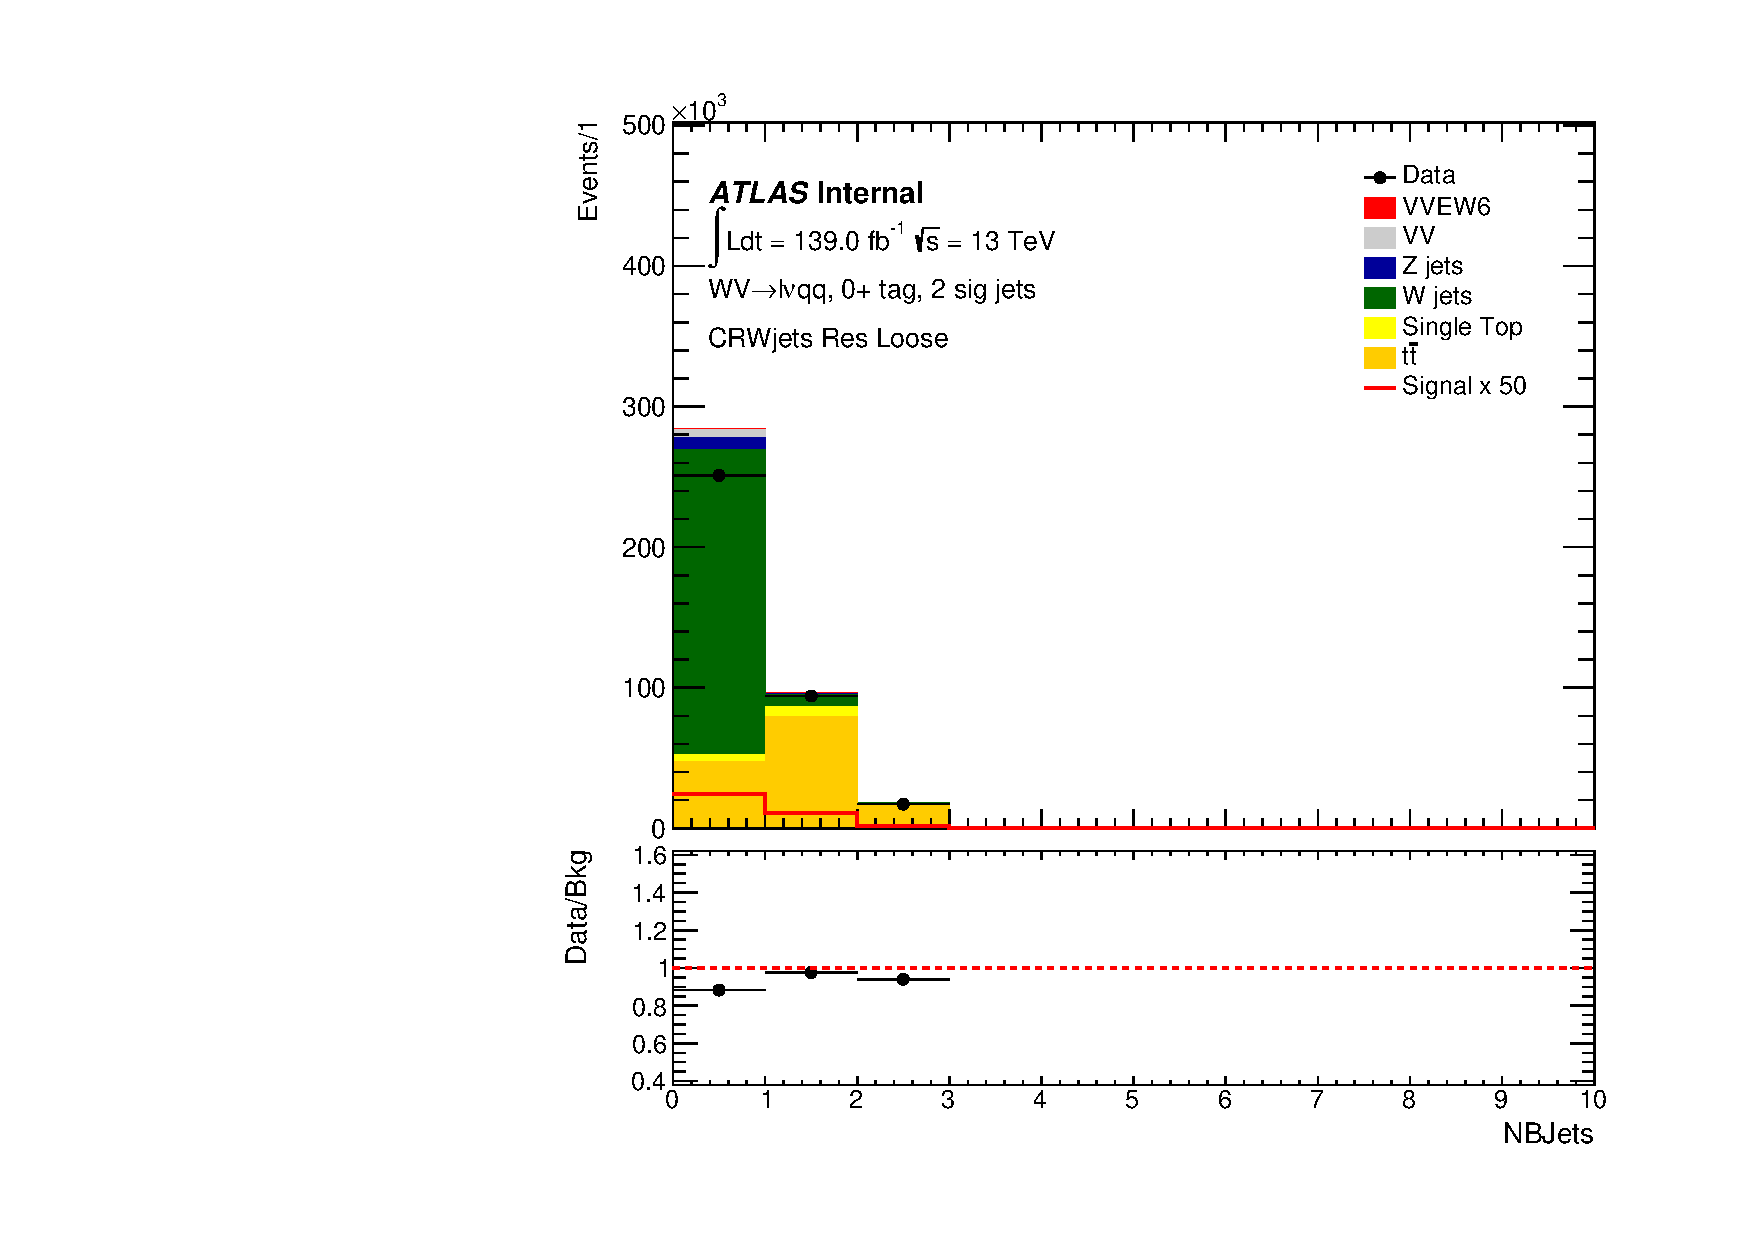
\includegraphics[width=0.3\textwidth]{figures/CRPlots/CRWjets_Res_Loose/stacked_plot_NBJets.pdf}}
    \subfloat[]{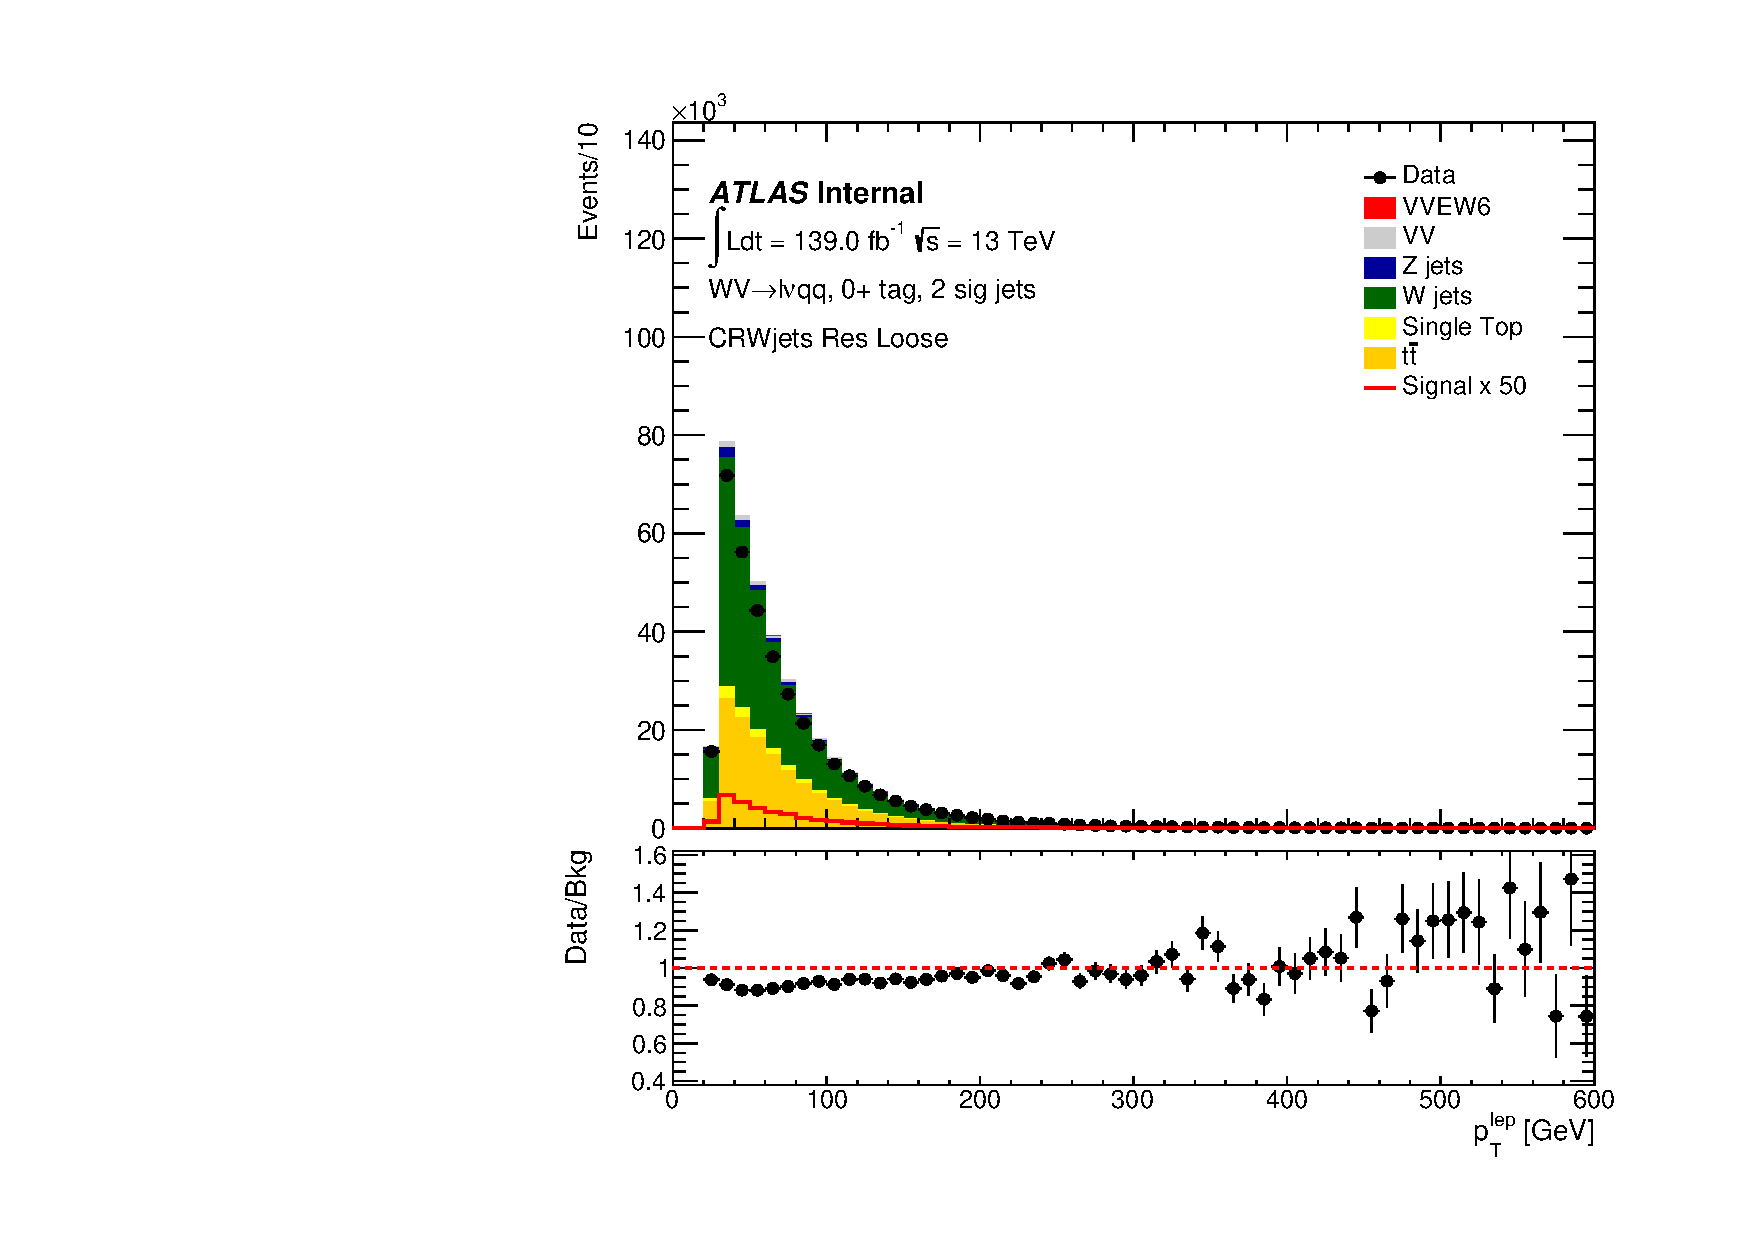
\includegraphics[width=0.3\textwidth]{figures/CRPlots/CRWjets_Res_Loose/stacked_plot_lep_pt.pdf}}  %%\\
    \caption{Data-MC checks for the resolved loose \Wjets control region in the \olep channel.}
    \label{fig:CRWjetResLoosePlots1Lep}
\end{figure}


\begin{figure}[ht]
    \centering
    \subfloat[]{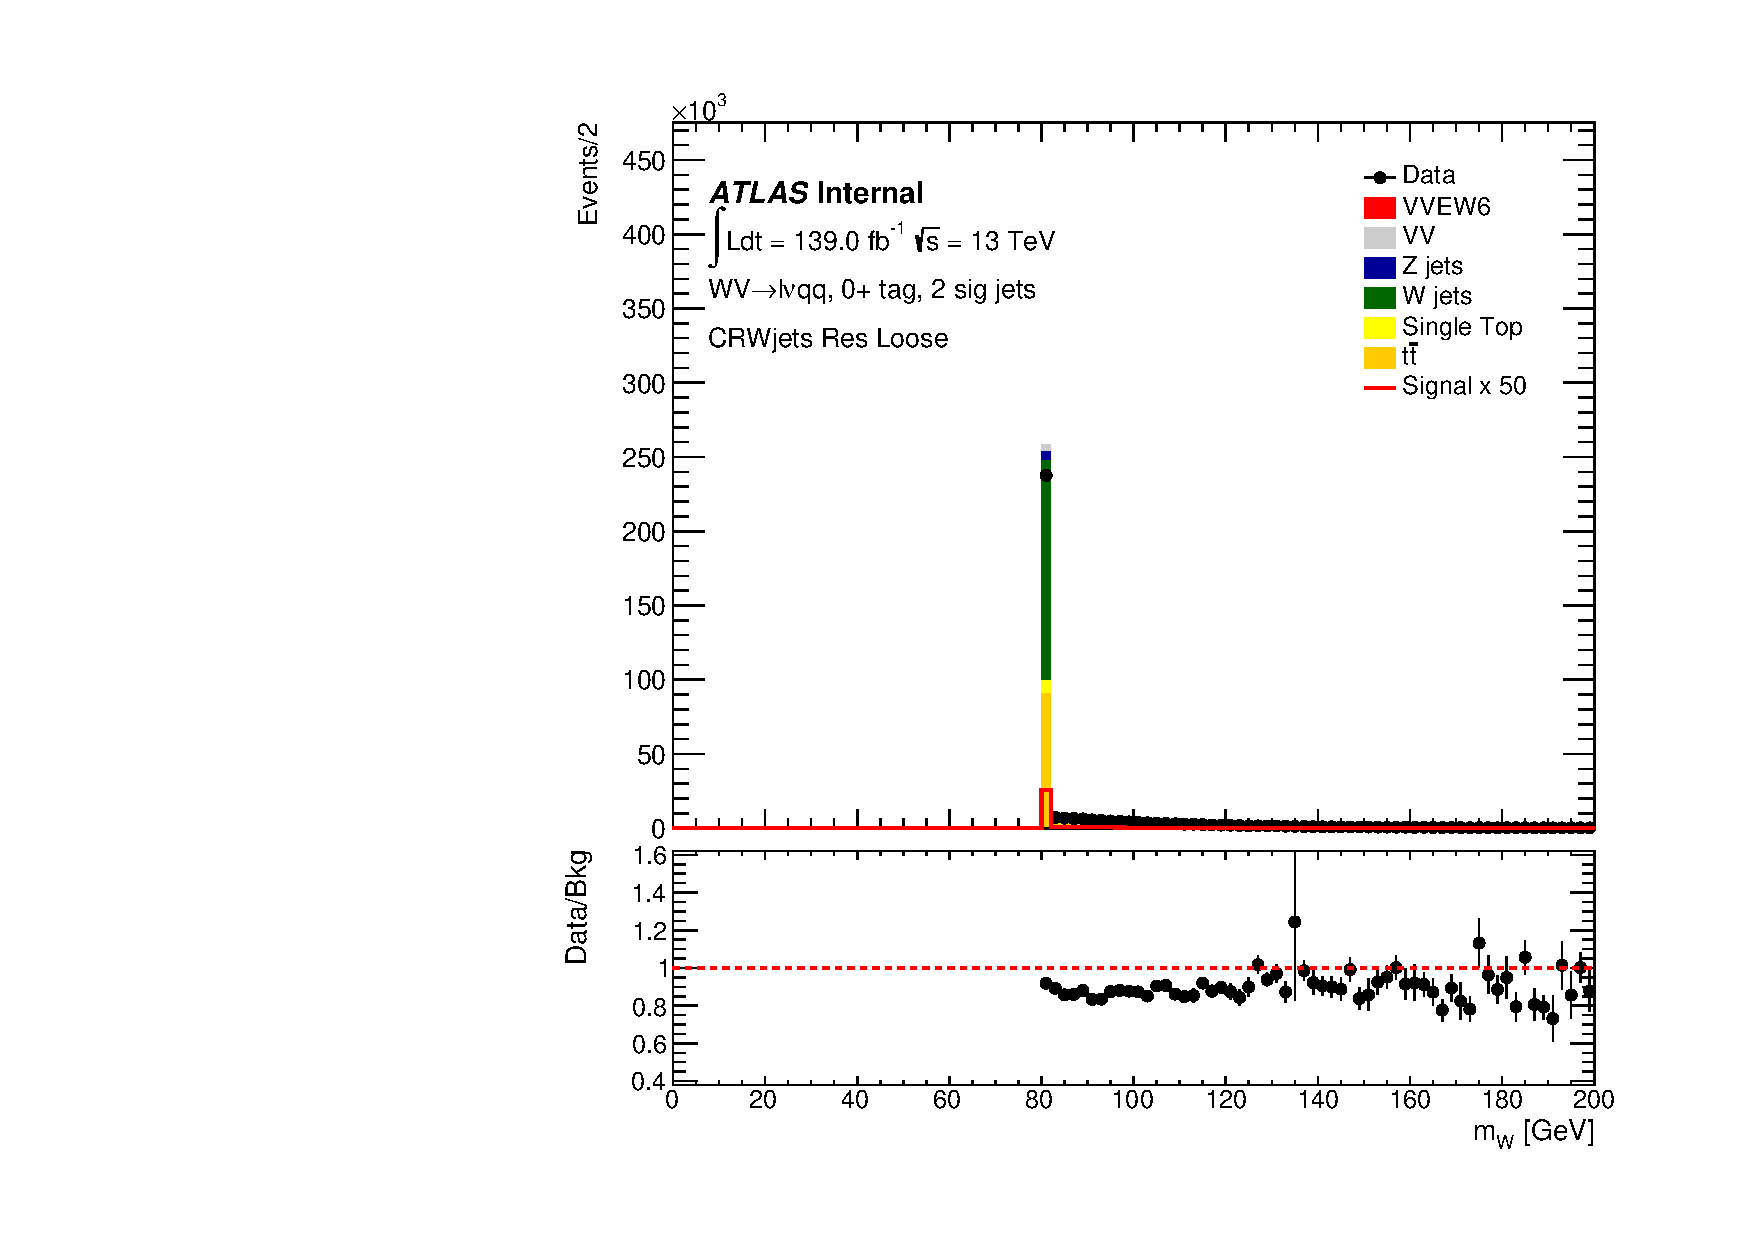
\includegraphics[width=0.3\textwidth]{figures/CRPlots/CRWjets_Res_Loose/stacked_plot_W_m.pdf}}
    \subfloat[]{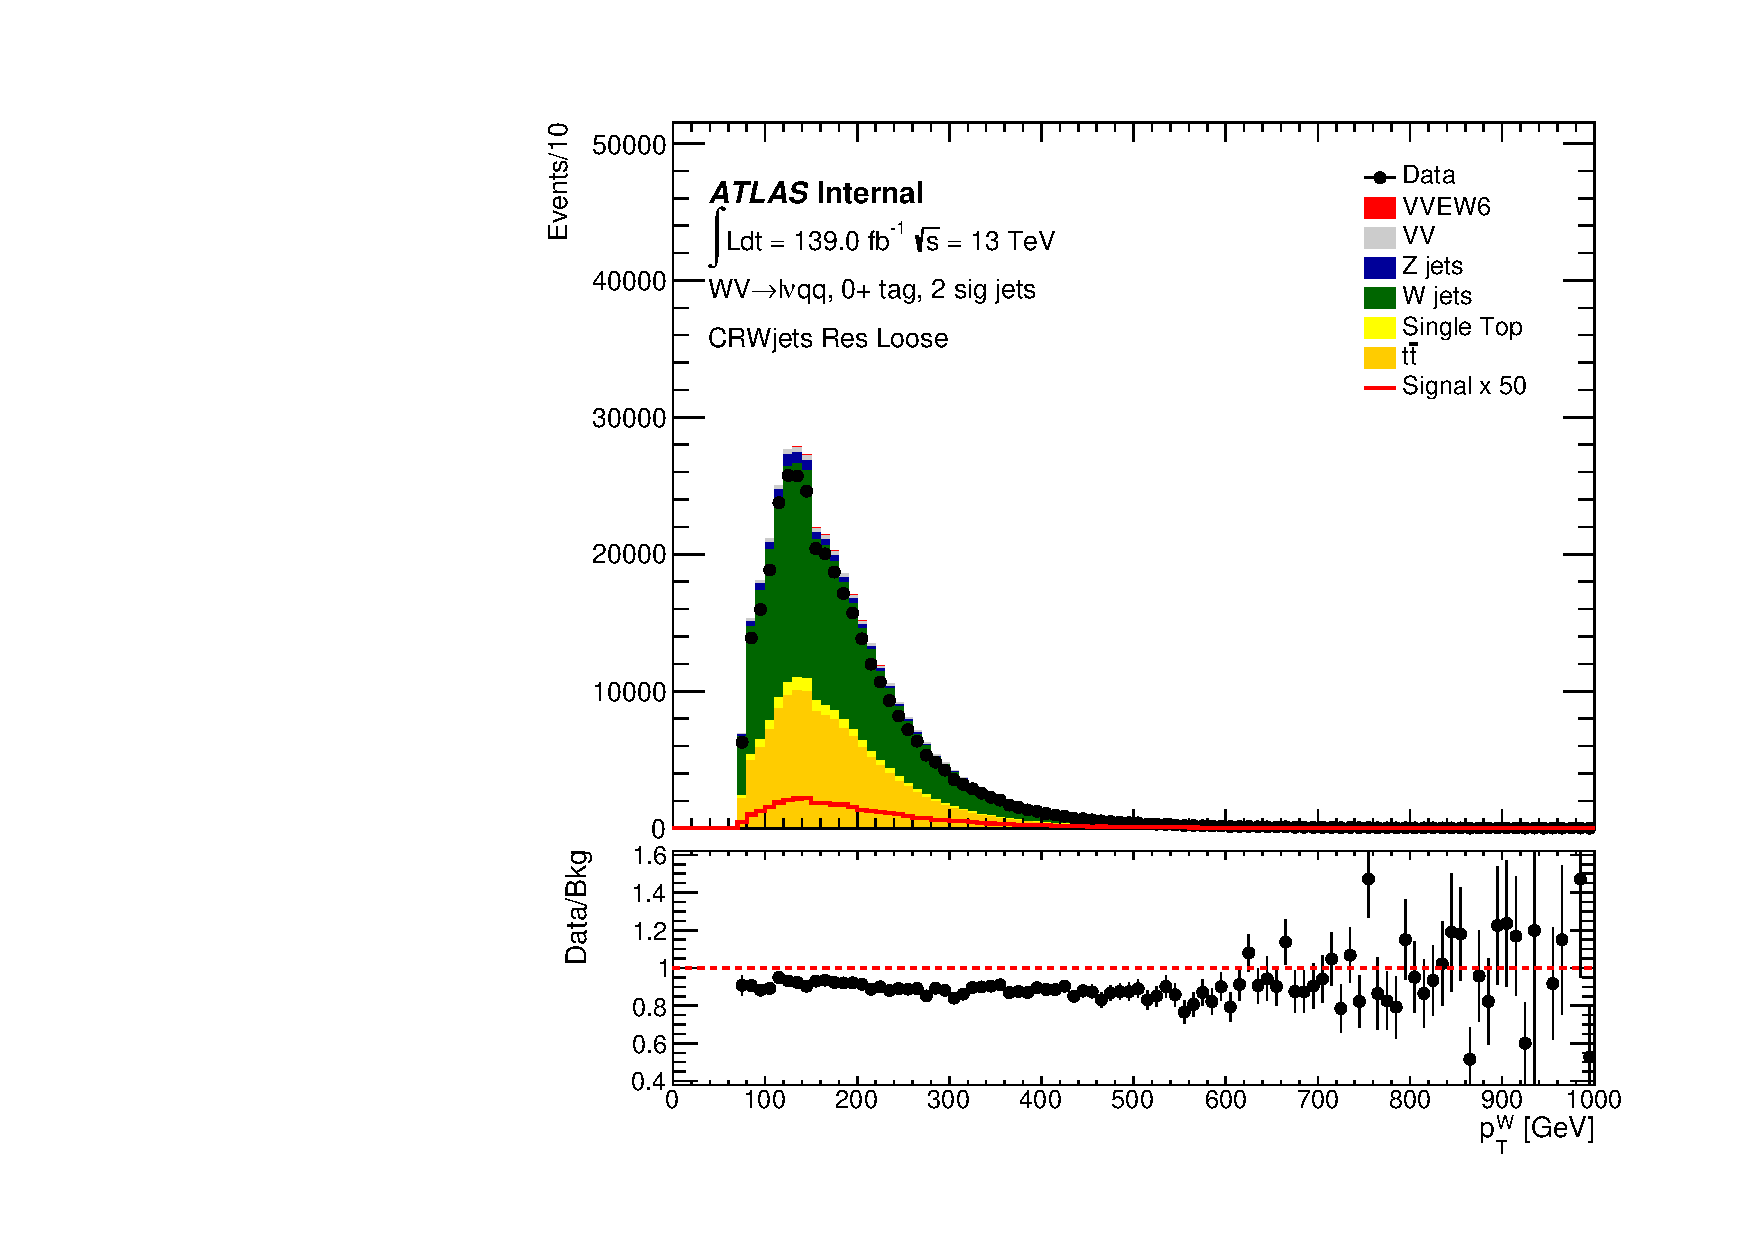
\includegraphics[width=0.3\textwidth]{figures/CRPlots/CRWjets_Res_Loose/stacked_plot_W_pt.pdf}}
    \subfloat[]{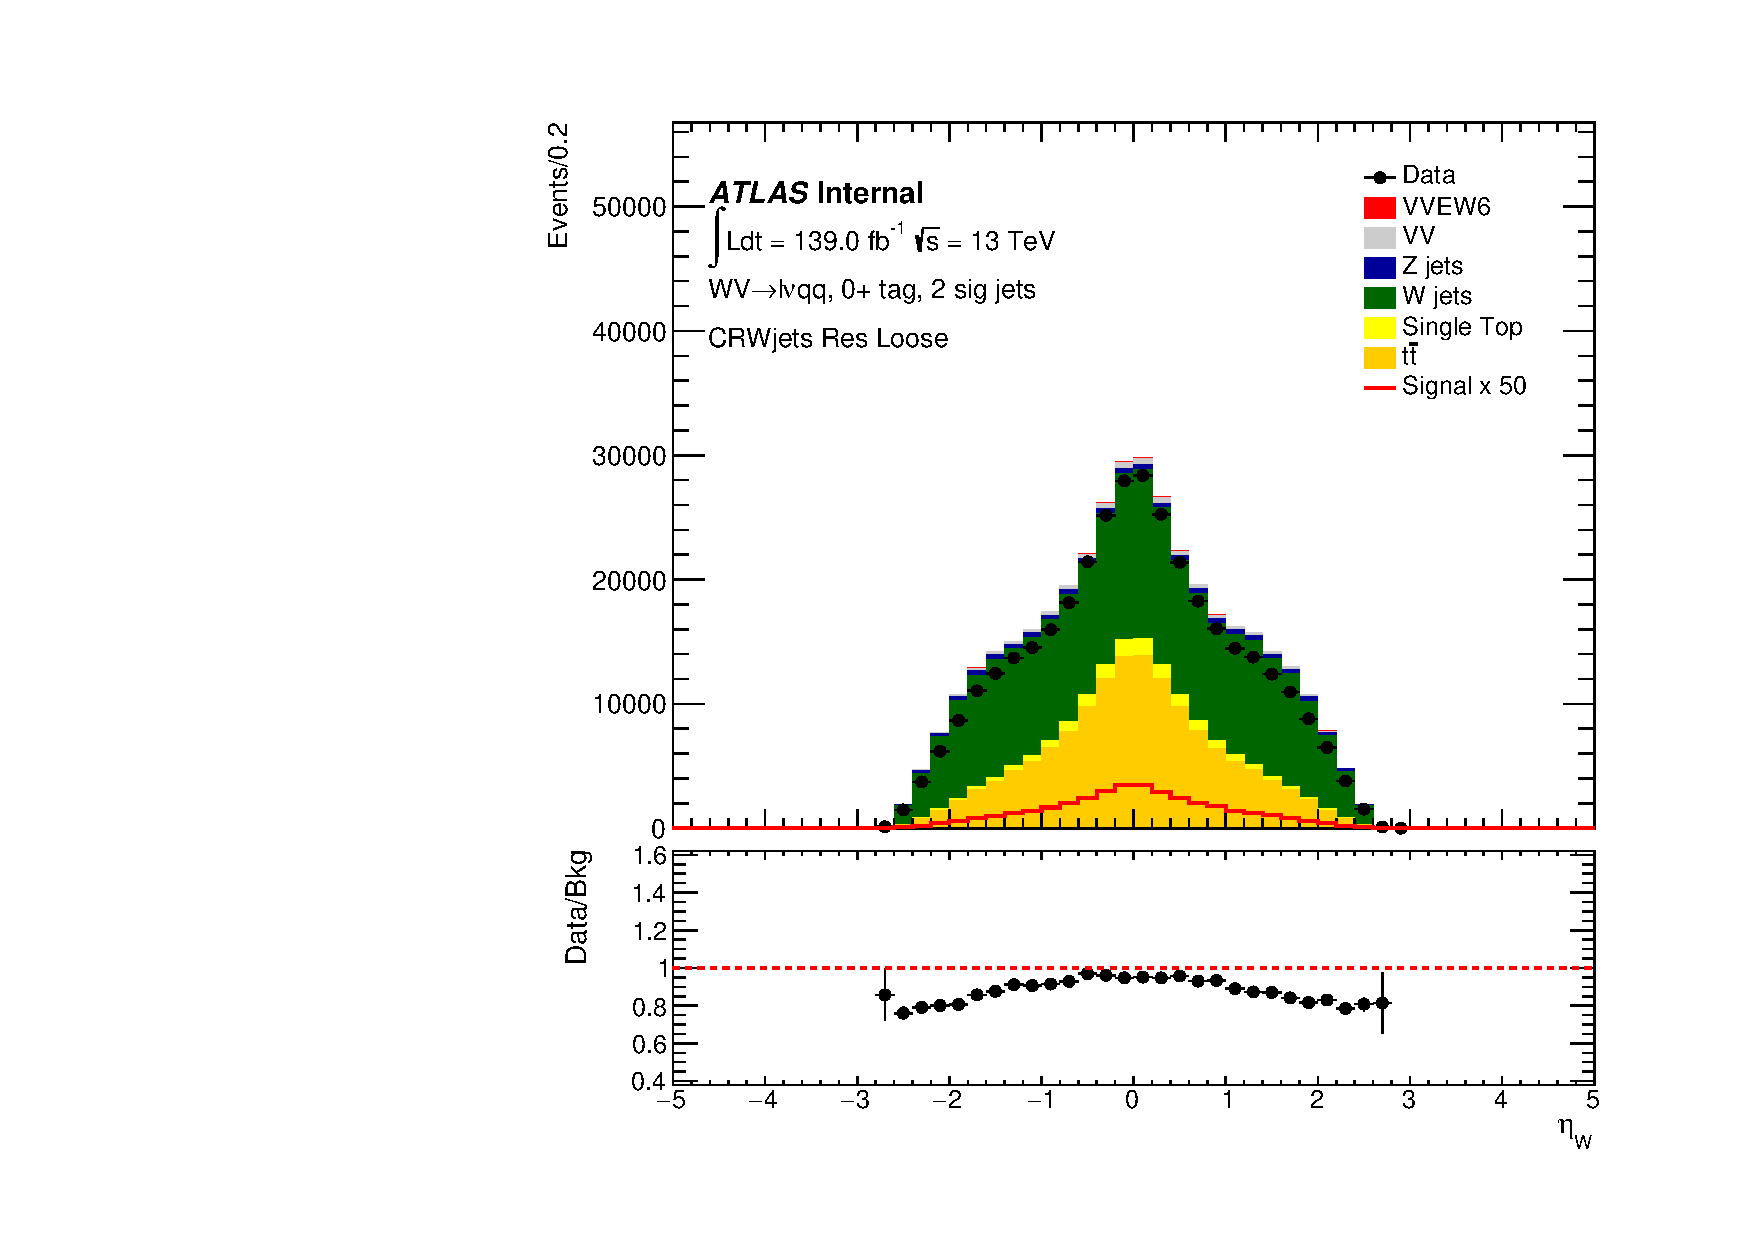
\includegraphics[width=0.3\textwidth]{figures/CRPlots/CRWjets_Res_Loose/stacked_plot_W_eta.pdf}} \\
    \subfloat[]{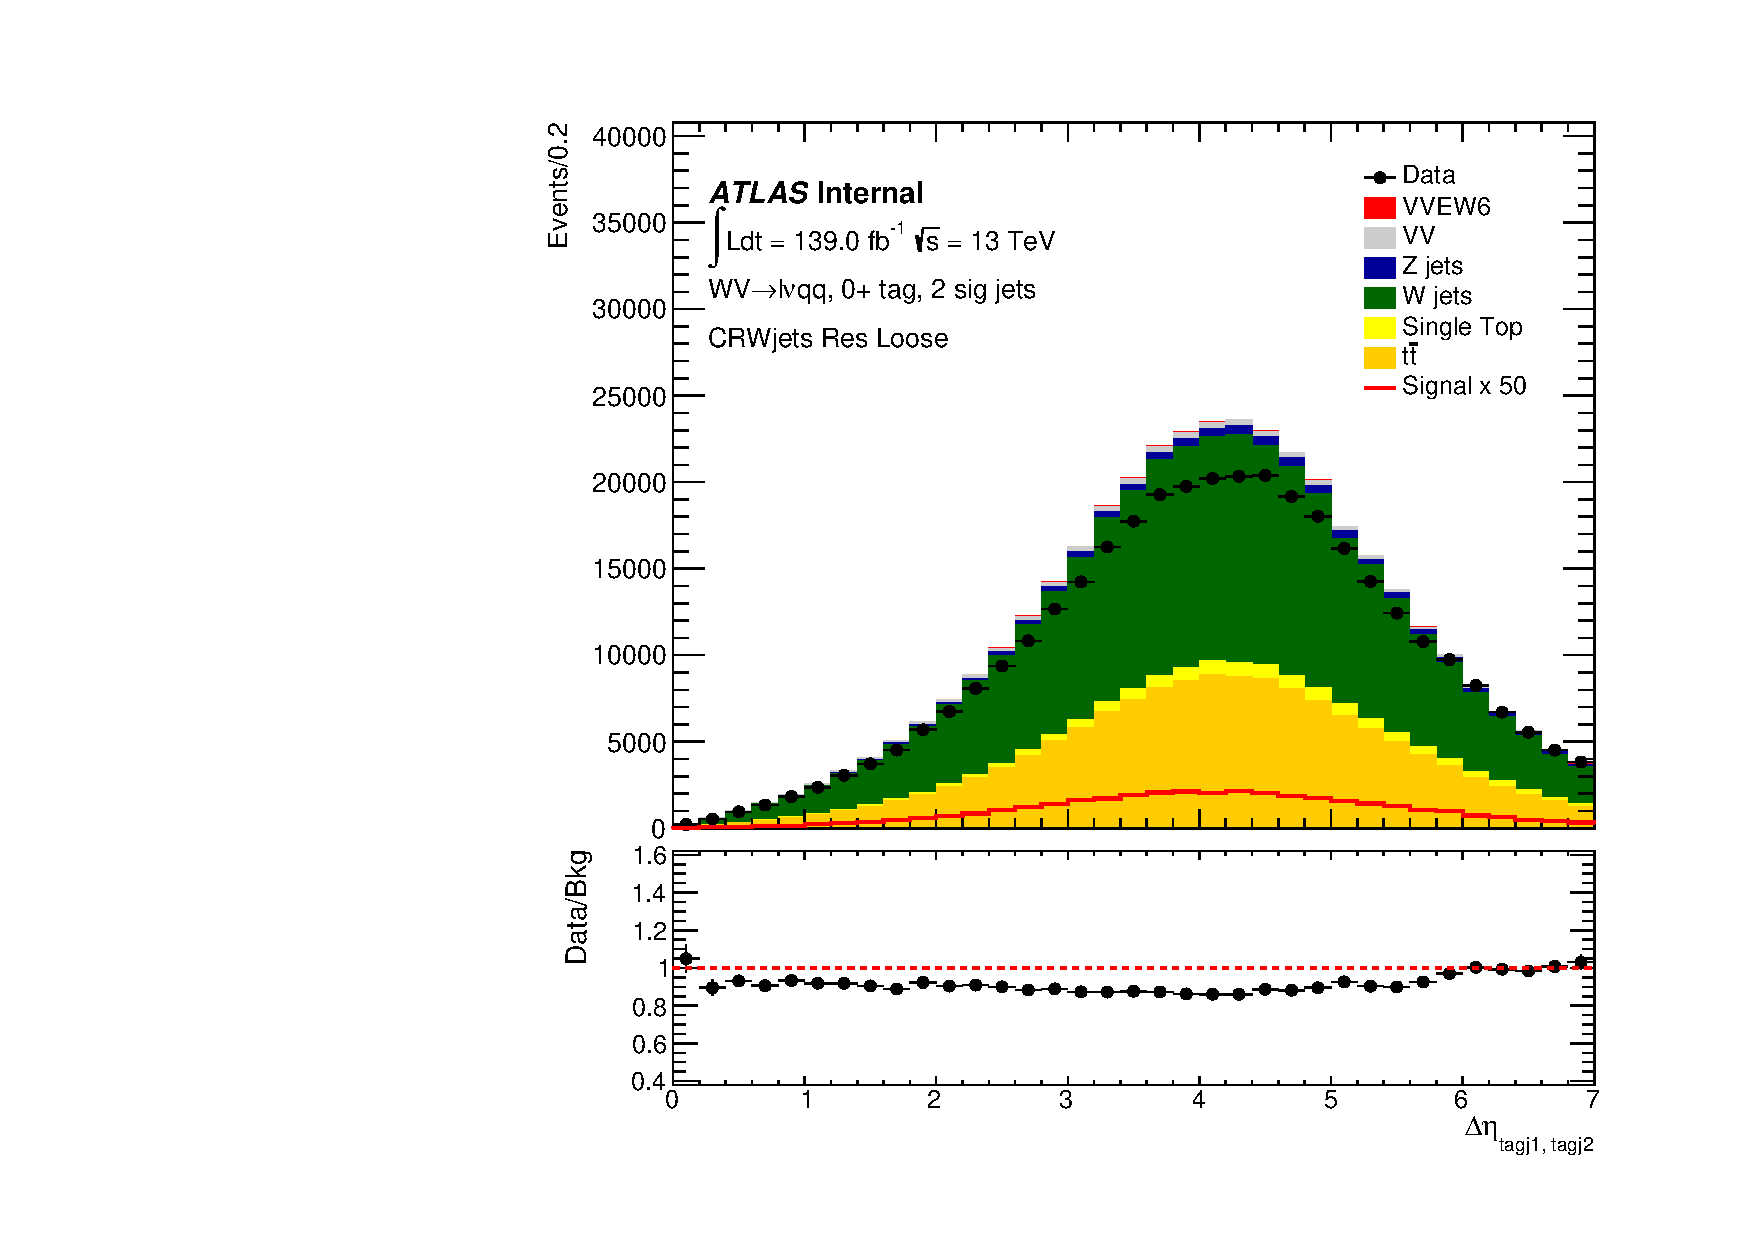
\includegraphics[width=0.3\textwidth]{figures/CRPlots/CRWjets_Res_Loose/stacked_plot_resolved_tagJdEta.pdf}}
    \subfloat[]{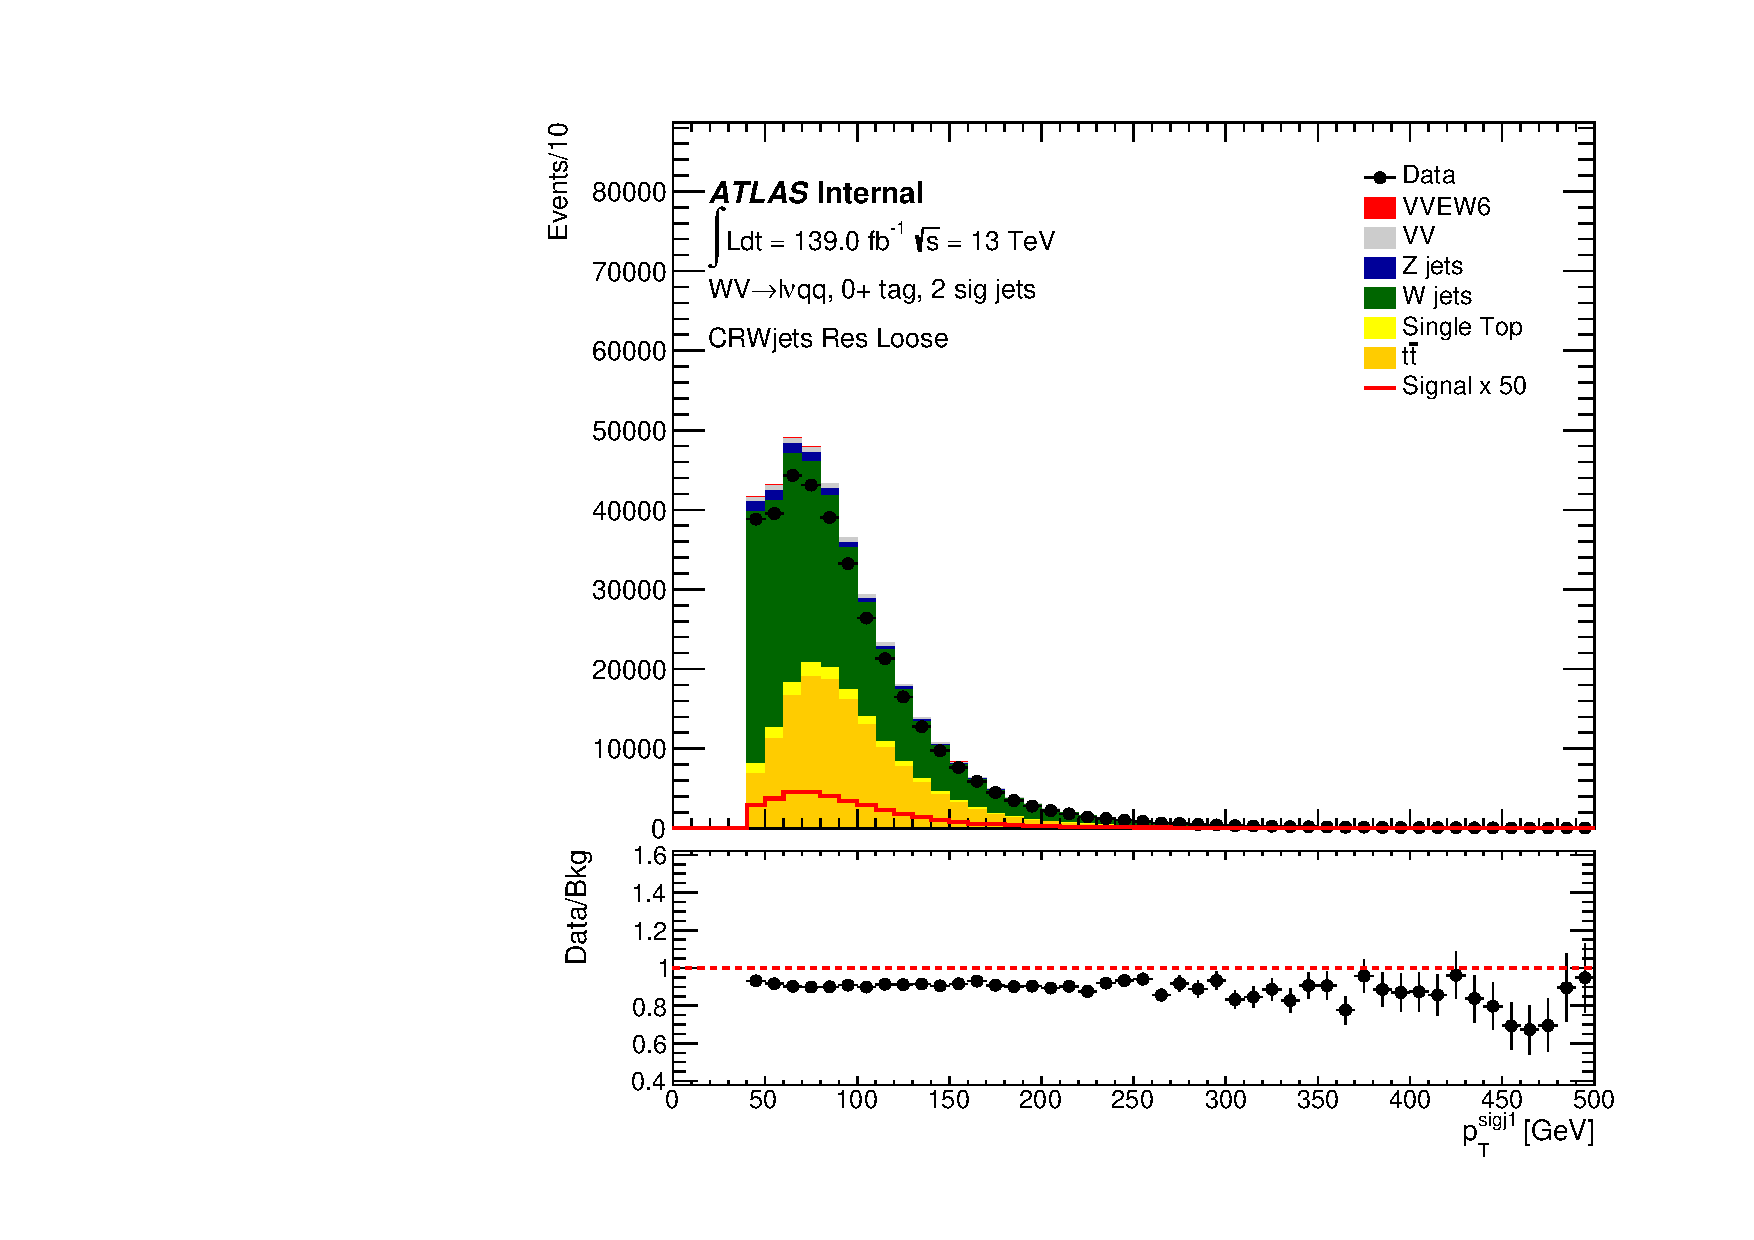
\includegraphics[width=0.3\textwidth]{figures/CRPlots/CRWjets_Res_Loose/stacked_plot_sigJ1_pt.pdf}}
    \subfloat[]{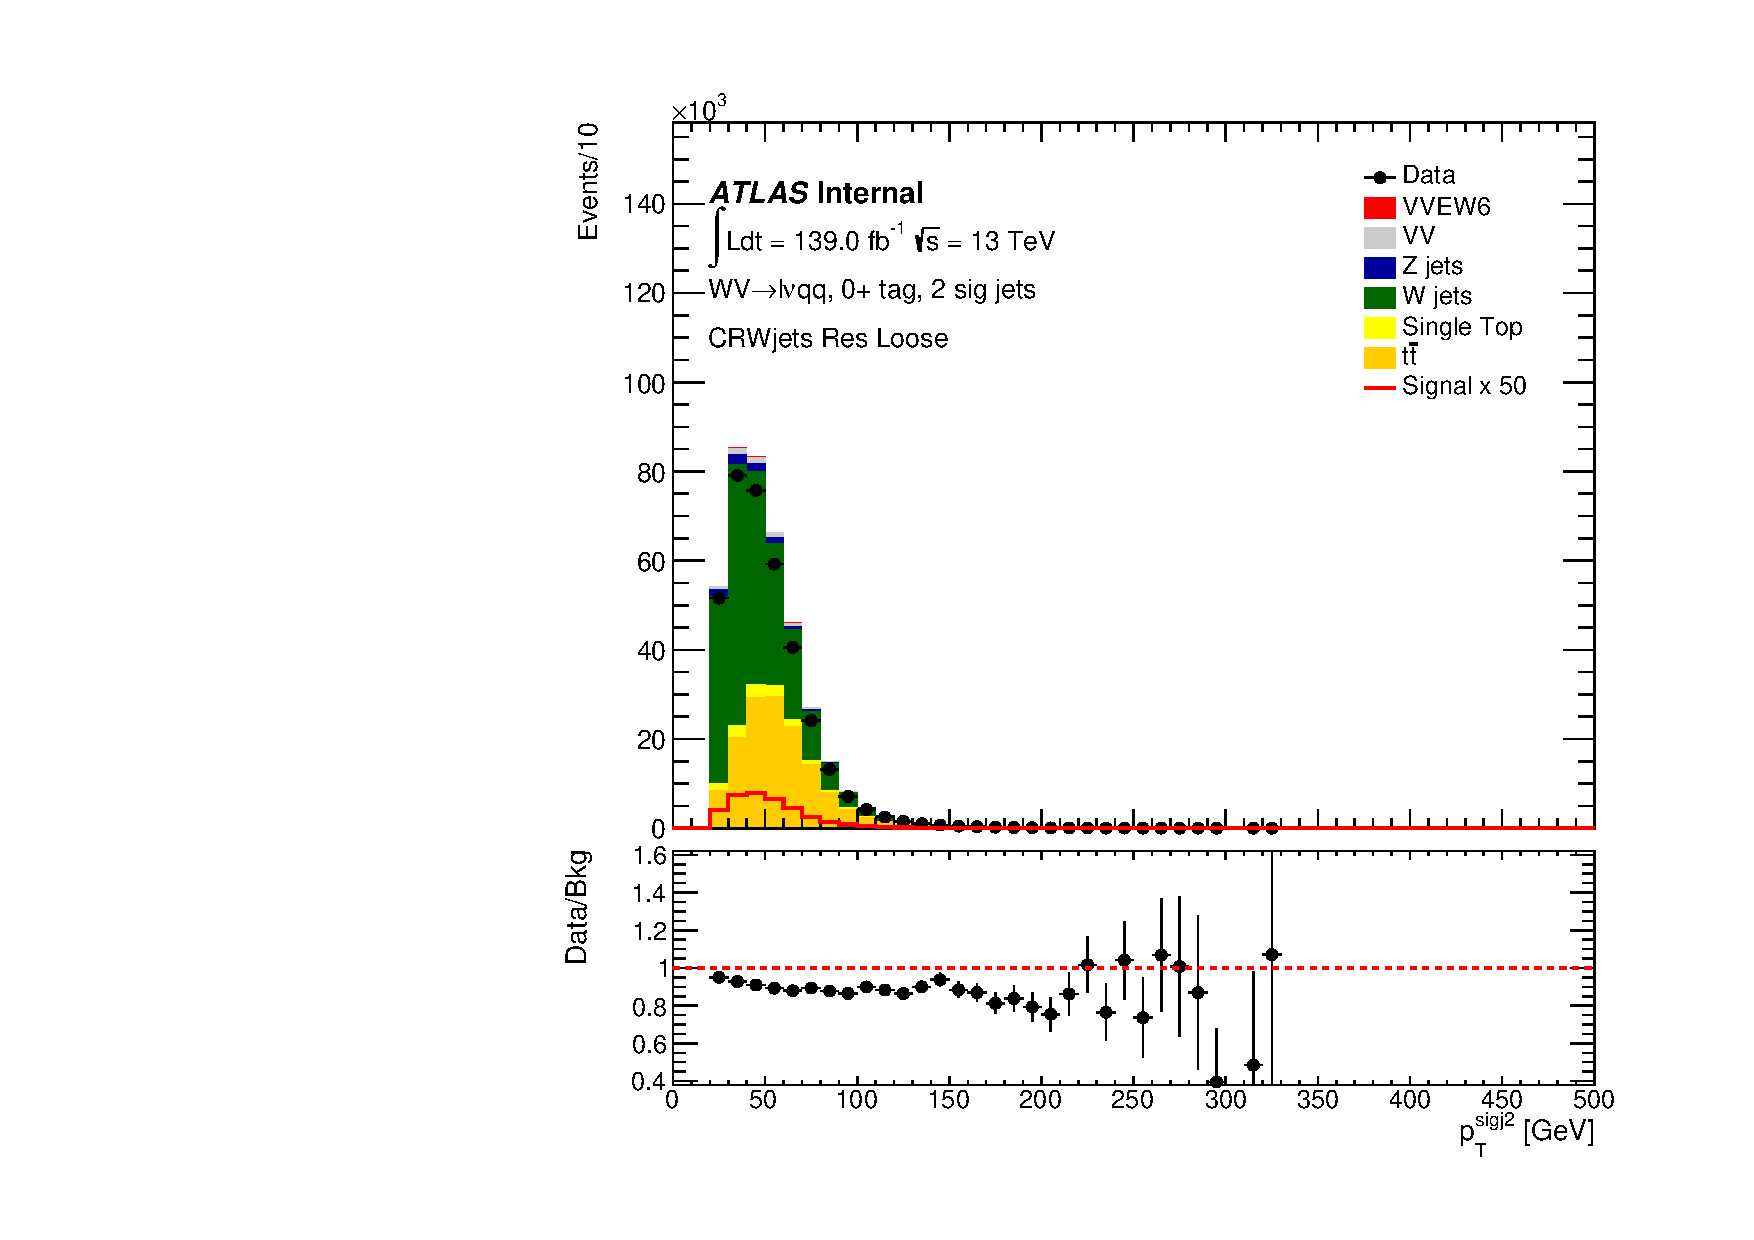
\includegraphics[width=0.3\textwidth]{figures/CRPlots/CRWjets_Res_Loose/stacked_plot_sigJ2_pt.pdf}} \\
    \subfloat[]{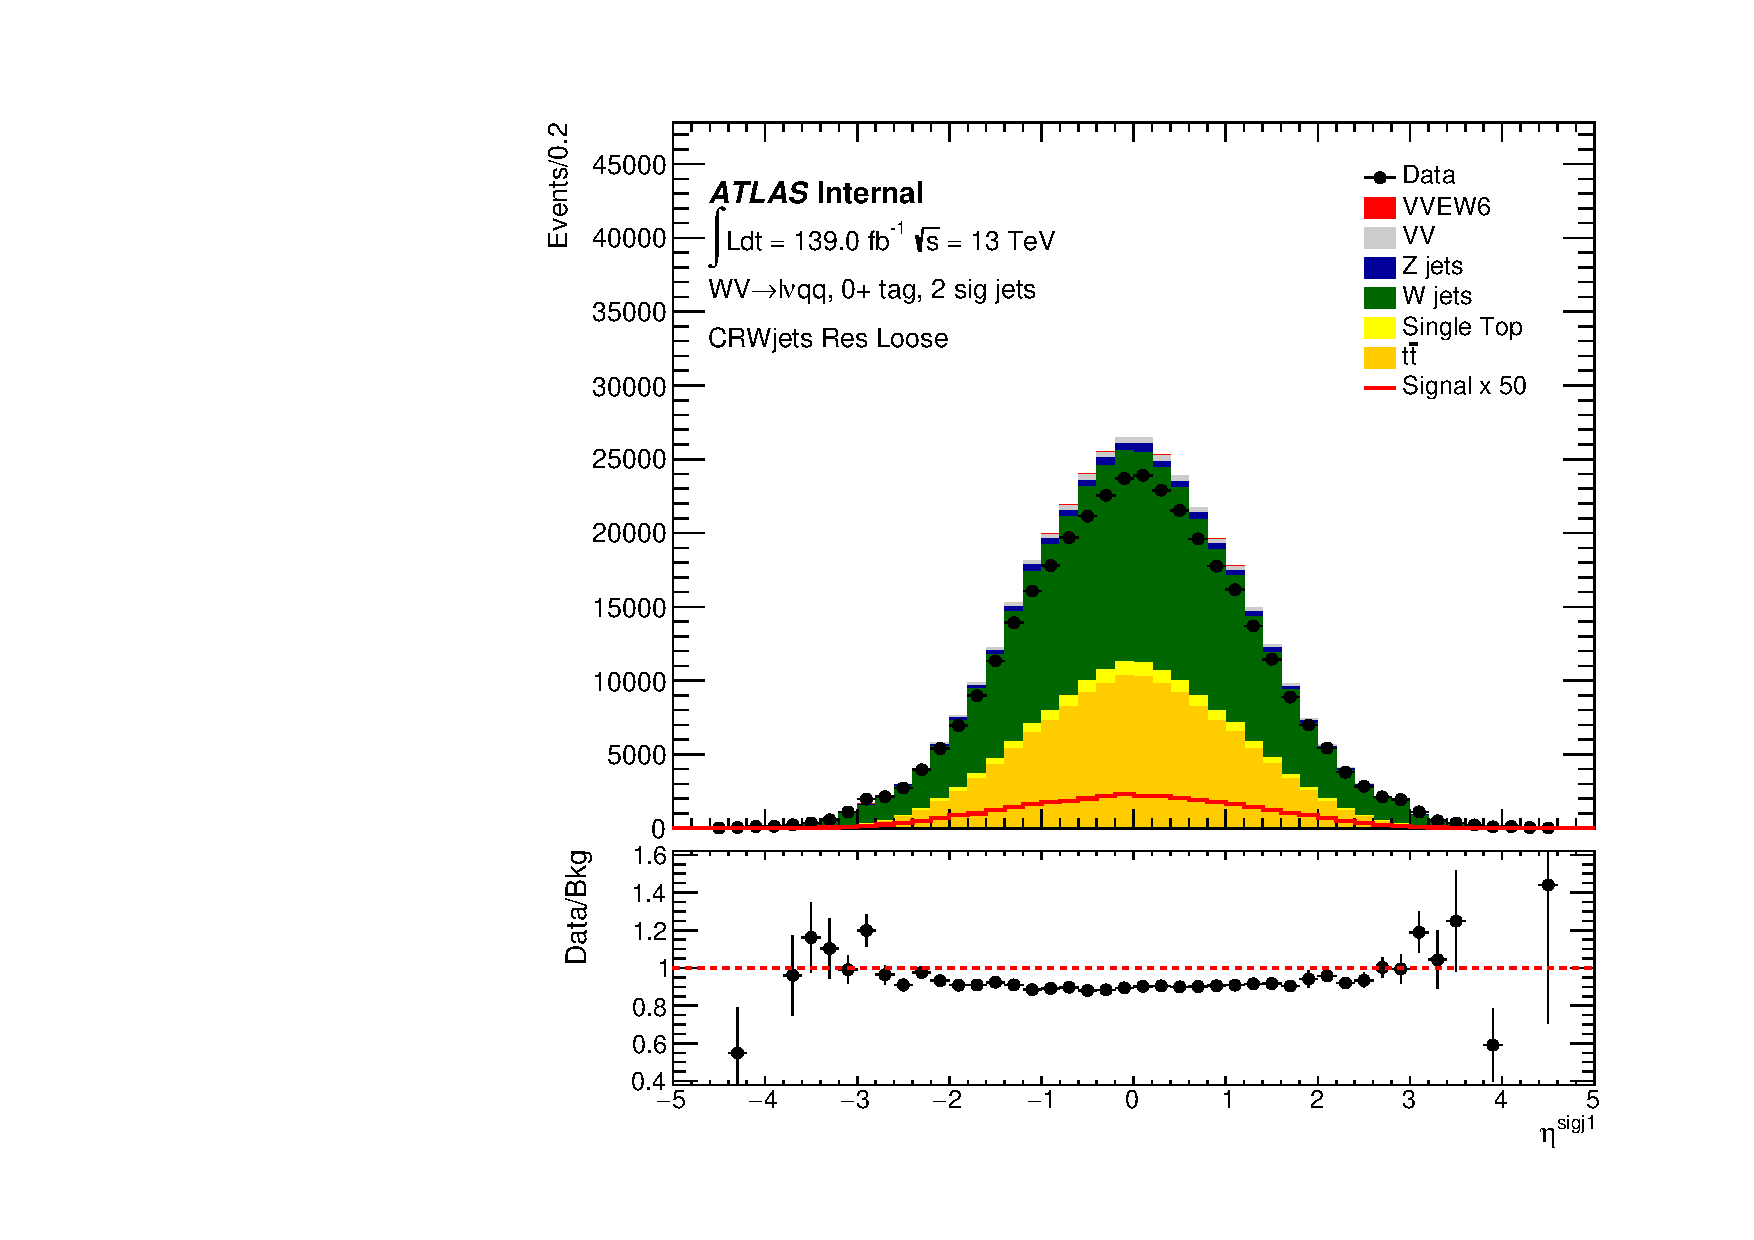
\includegraphics[width=0.3\textwidth]{figures/CRPlots/CRWjets_Res_Loose/stacked_plot_sigJ1_eta.pdf}}
    \subfloat[]{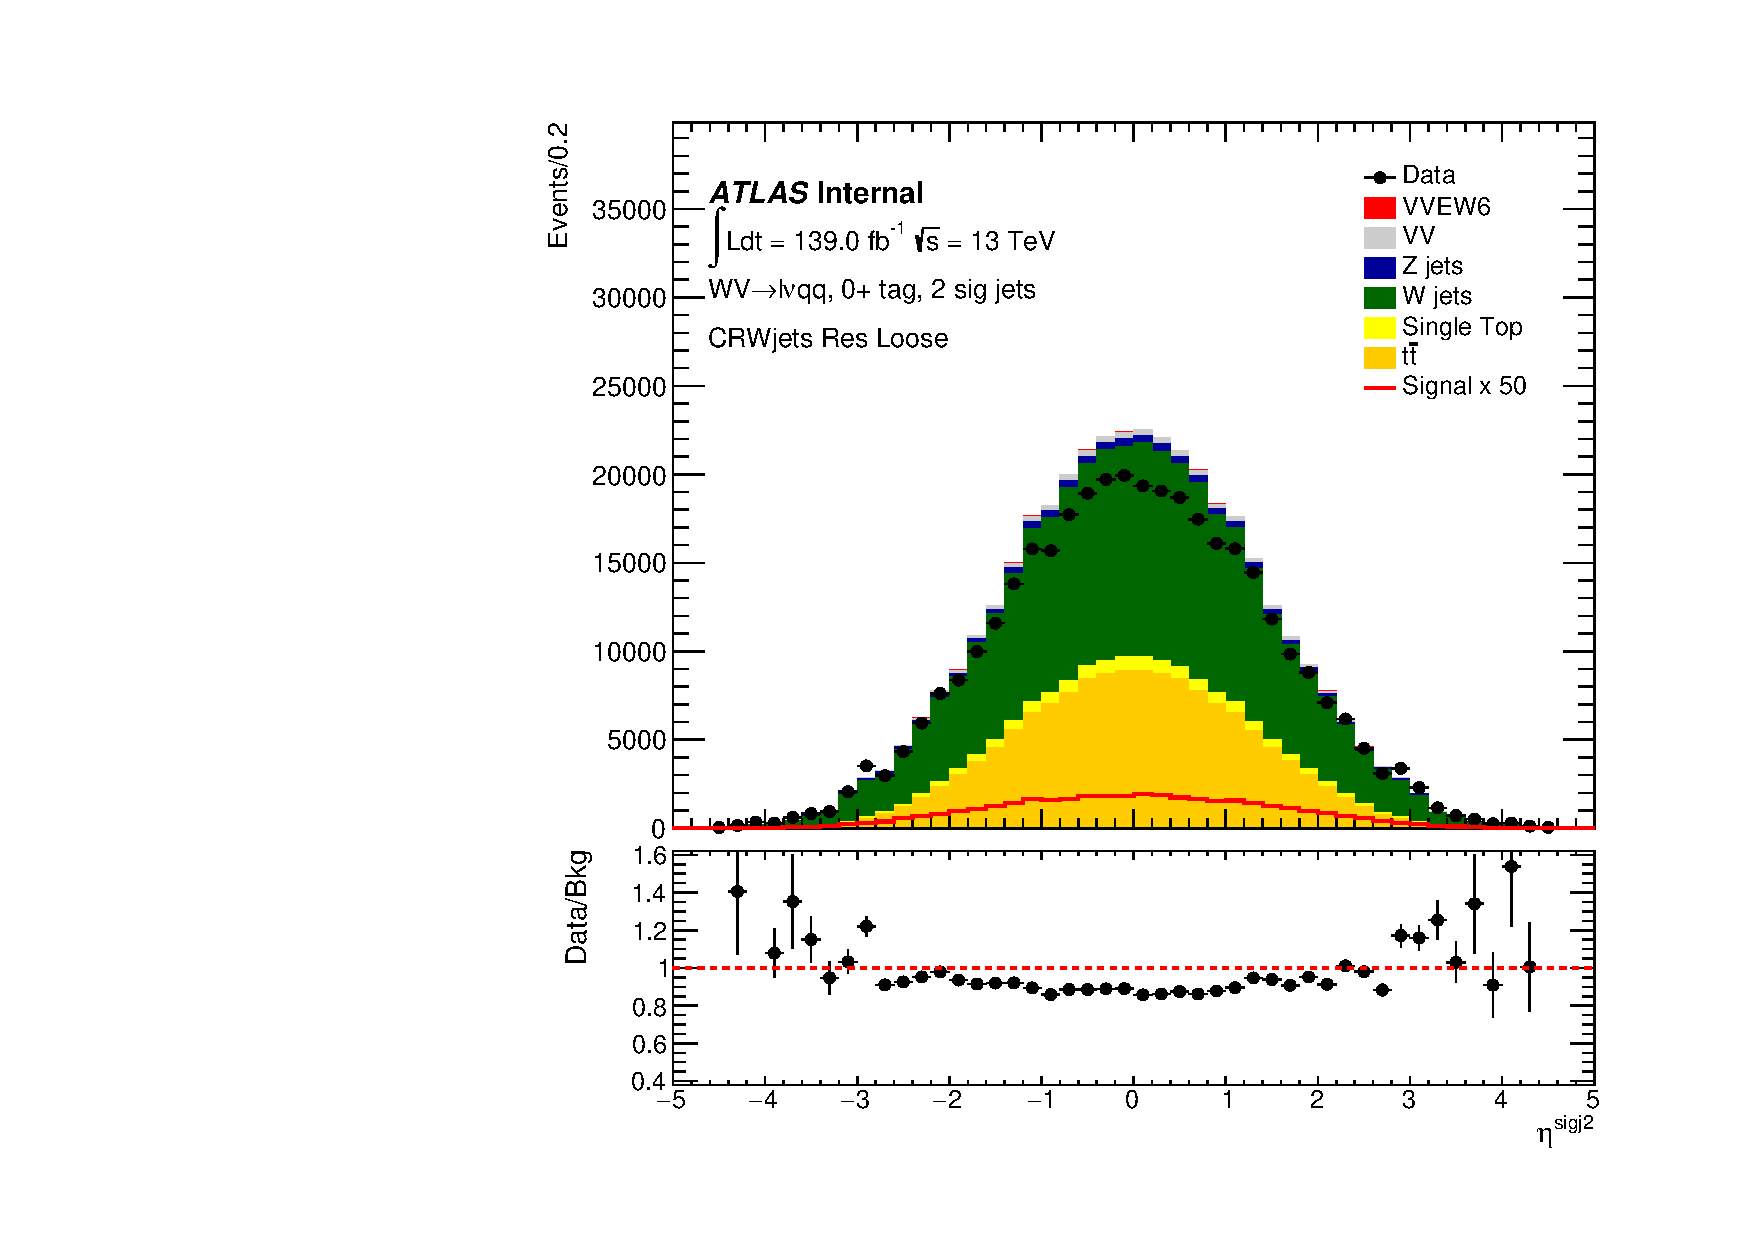
\includegraphics[width=0.3\textwidth]{figures/CRPlots/CRWjets_Res_Loose/stacked_plot_sigJ2_eta.pdf}} \\
    \subfloat[]{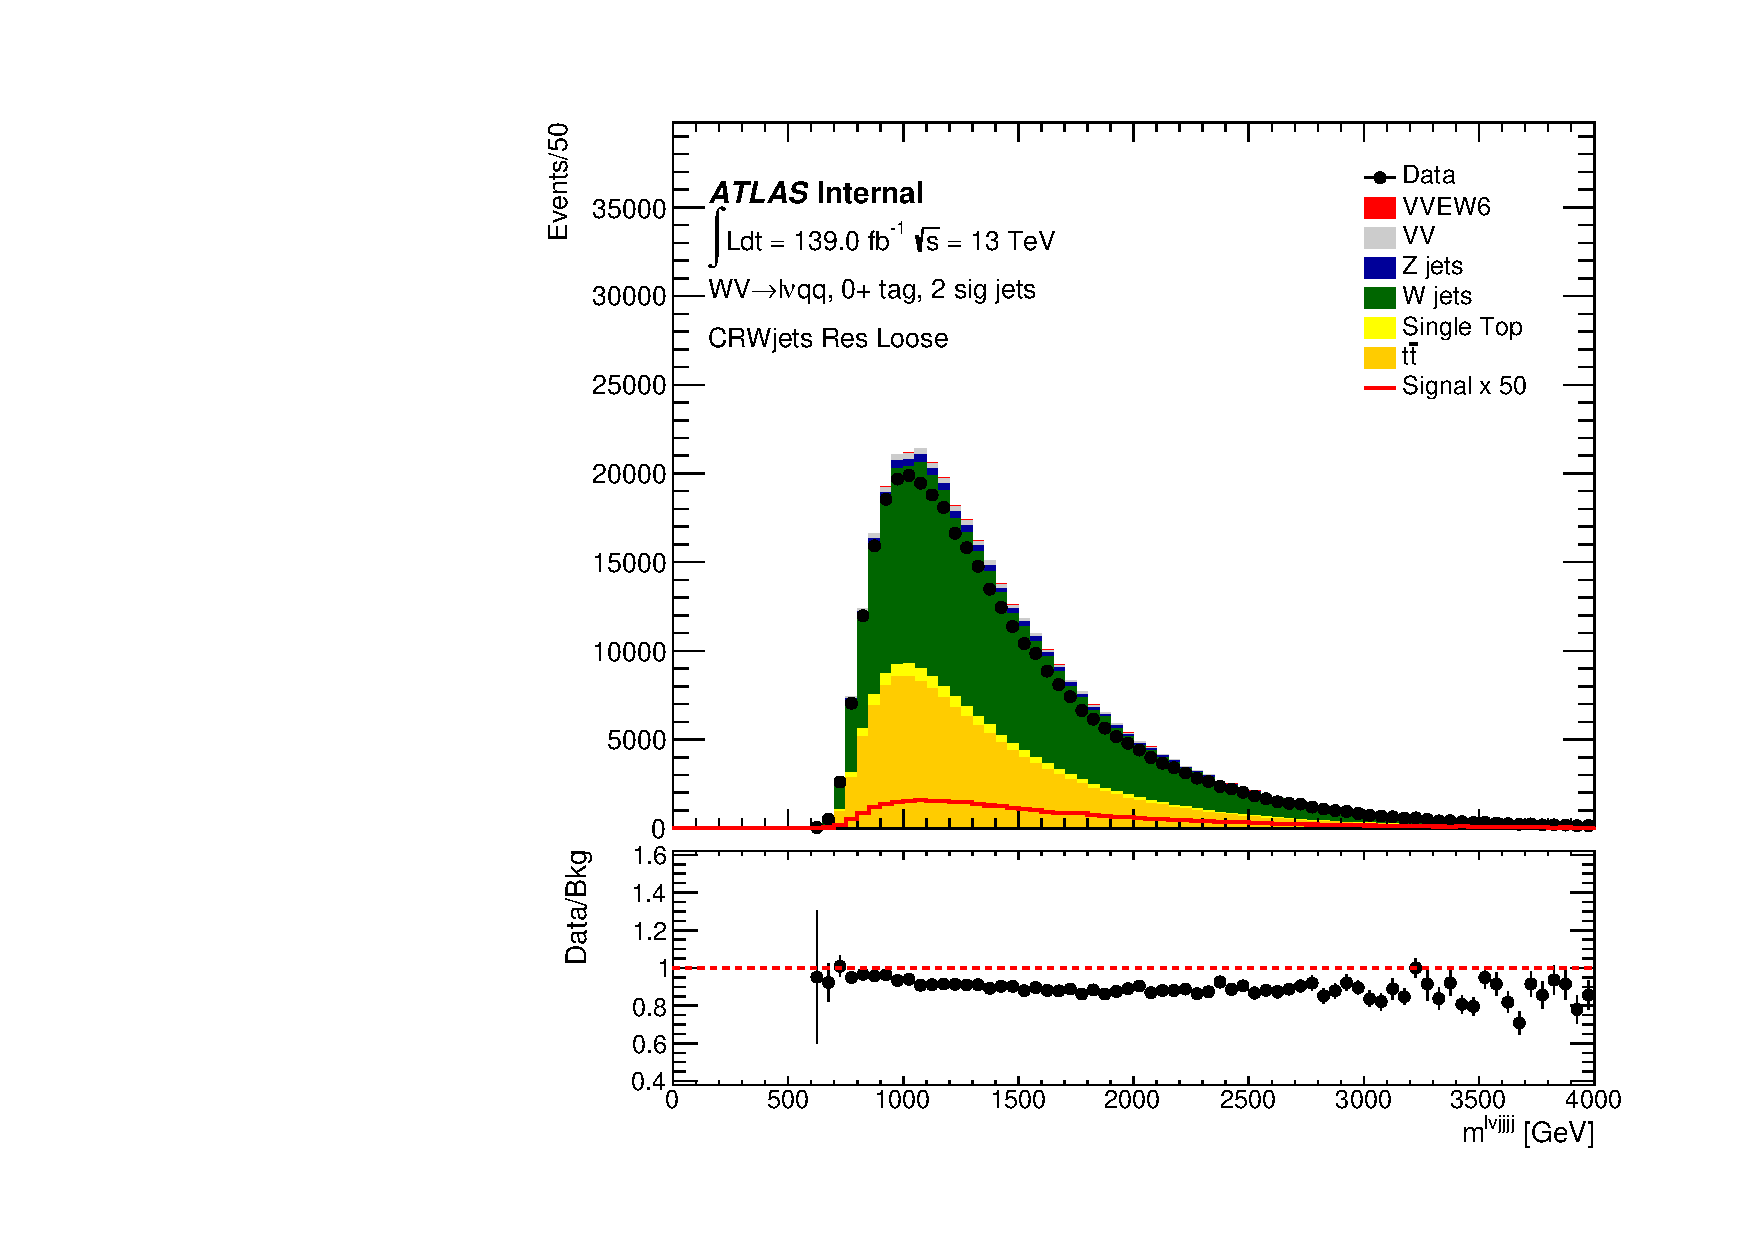
\includegraphics[width=0.3\textwidth]{figures/CRPlots/CRWjets_Res_Loose/stacked_plot_lvjjjjmass.pdf}}
    \subfloat[]{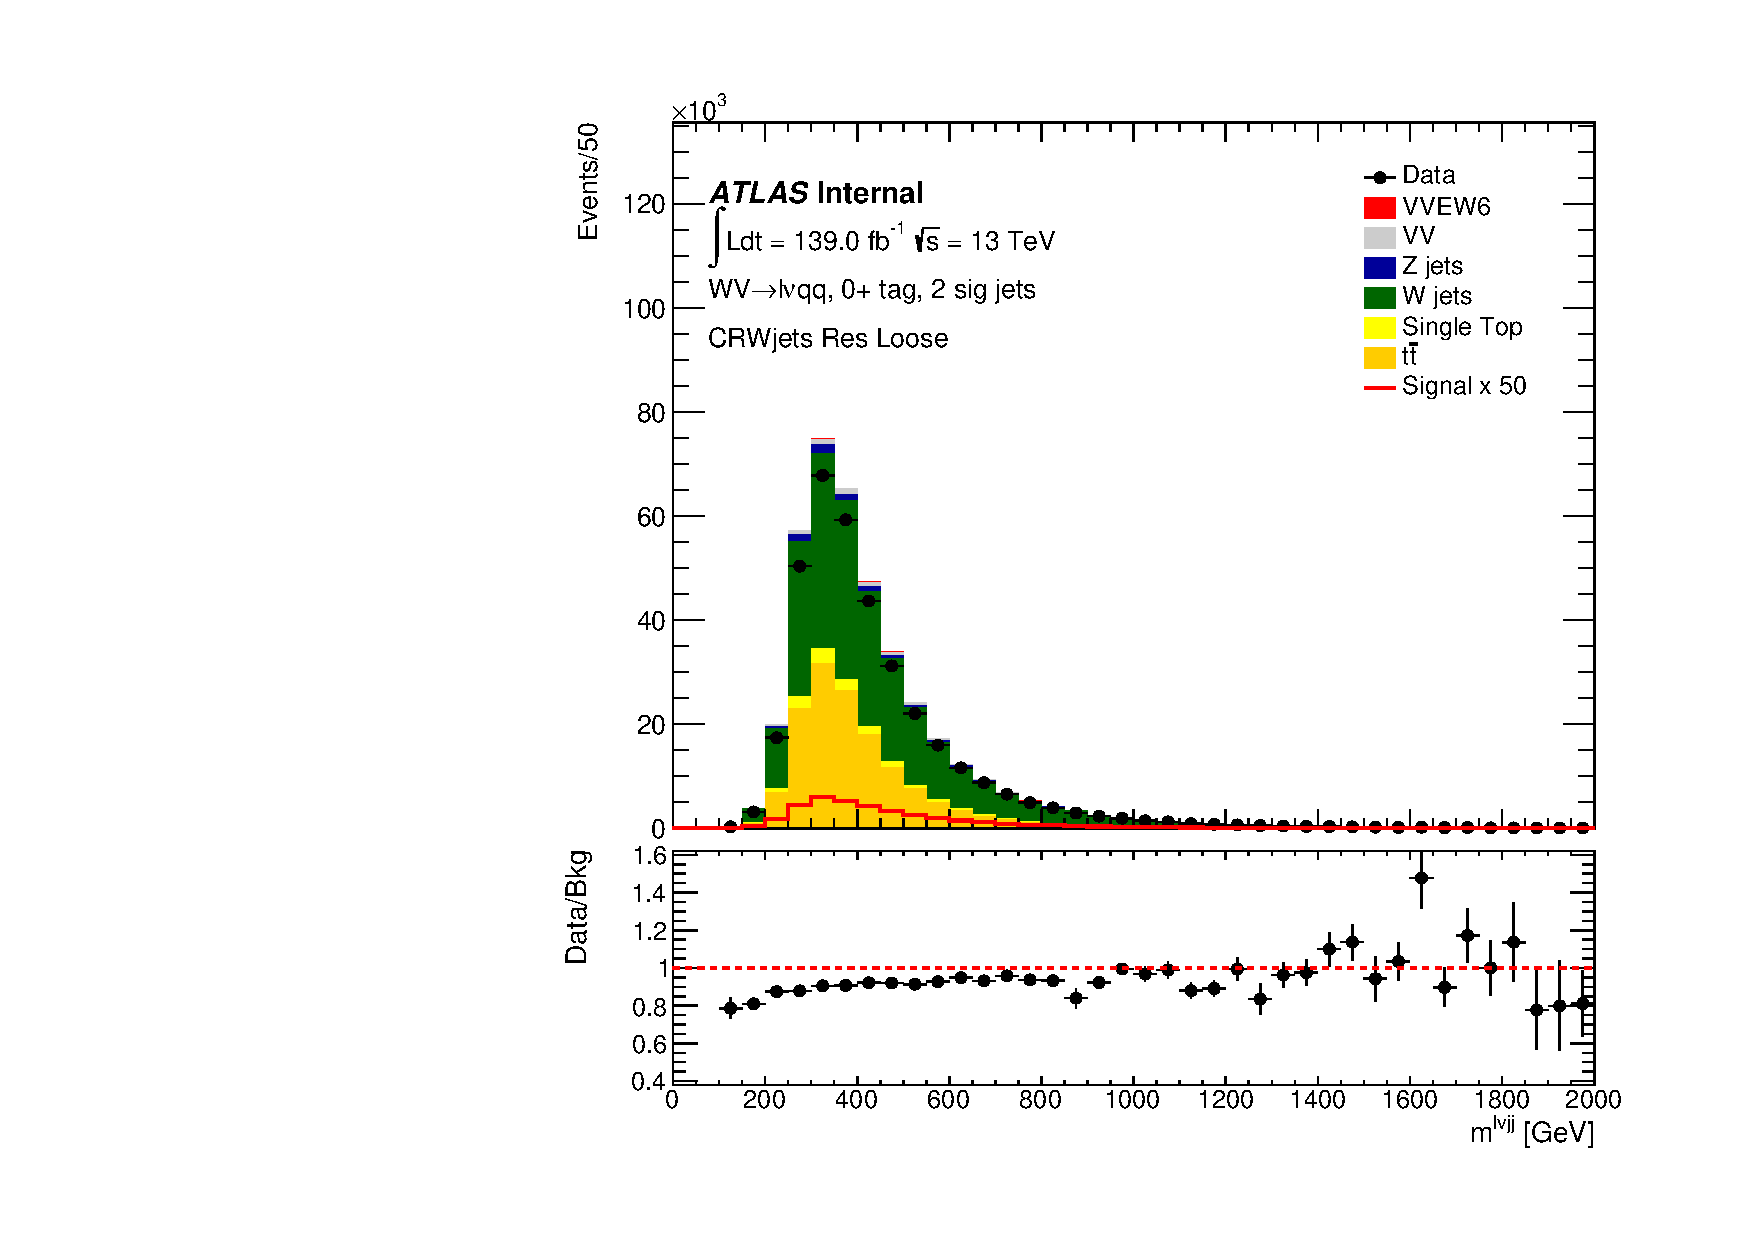
\includegraphics[width=0.3\textwidth]{figures/CRPlots/CRWjets_Res_Loose/stacked_plot_lvjjmass.pdf}}
    \subfloat[]{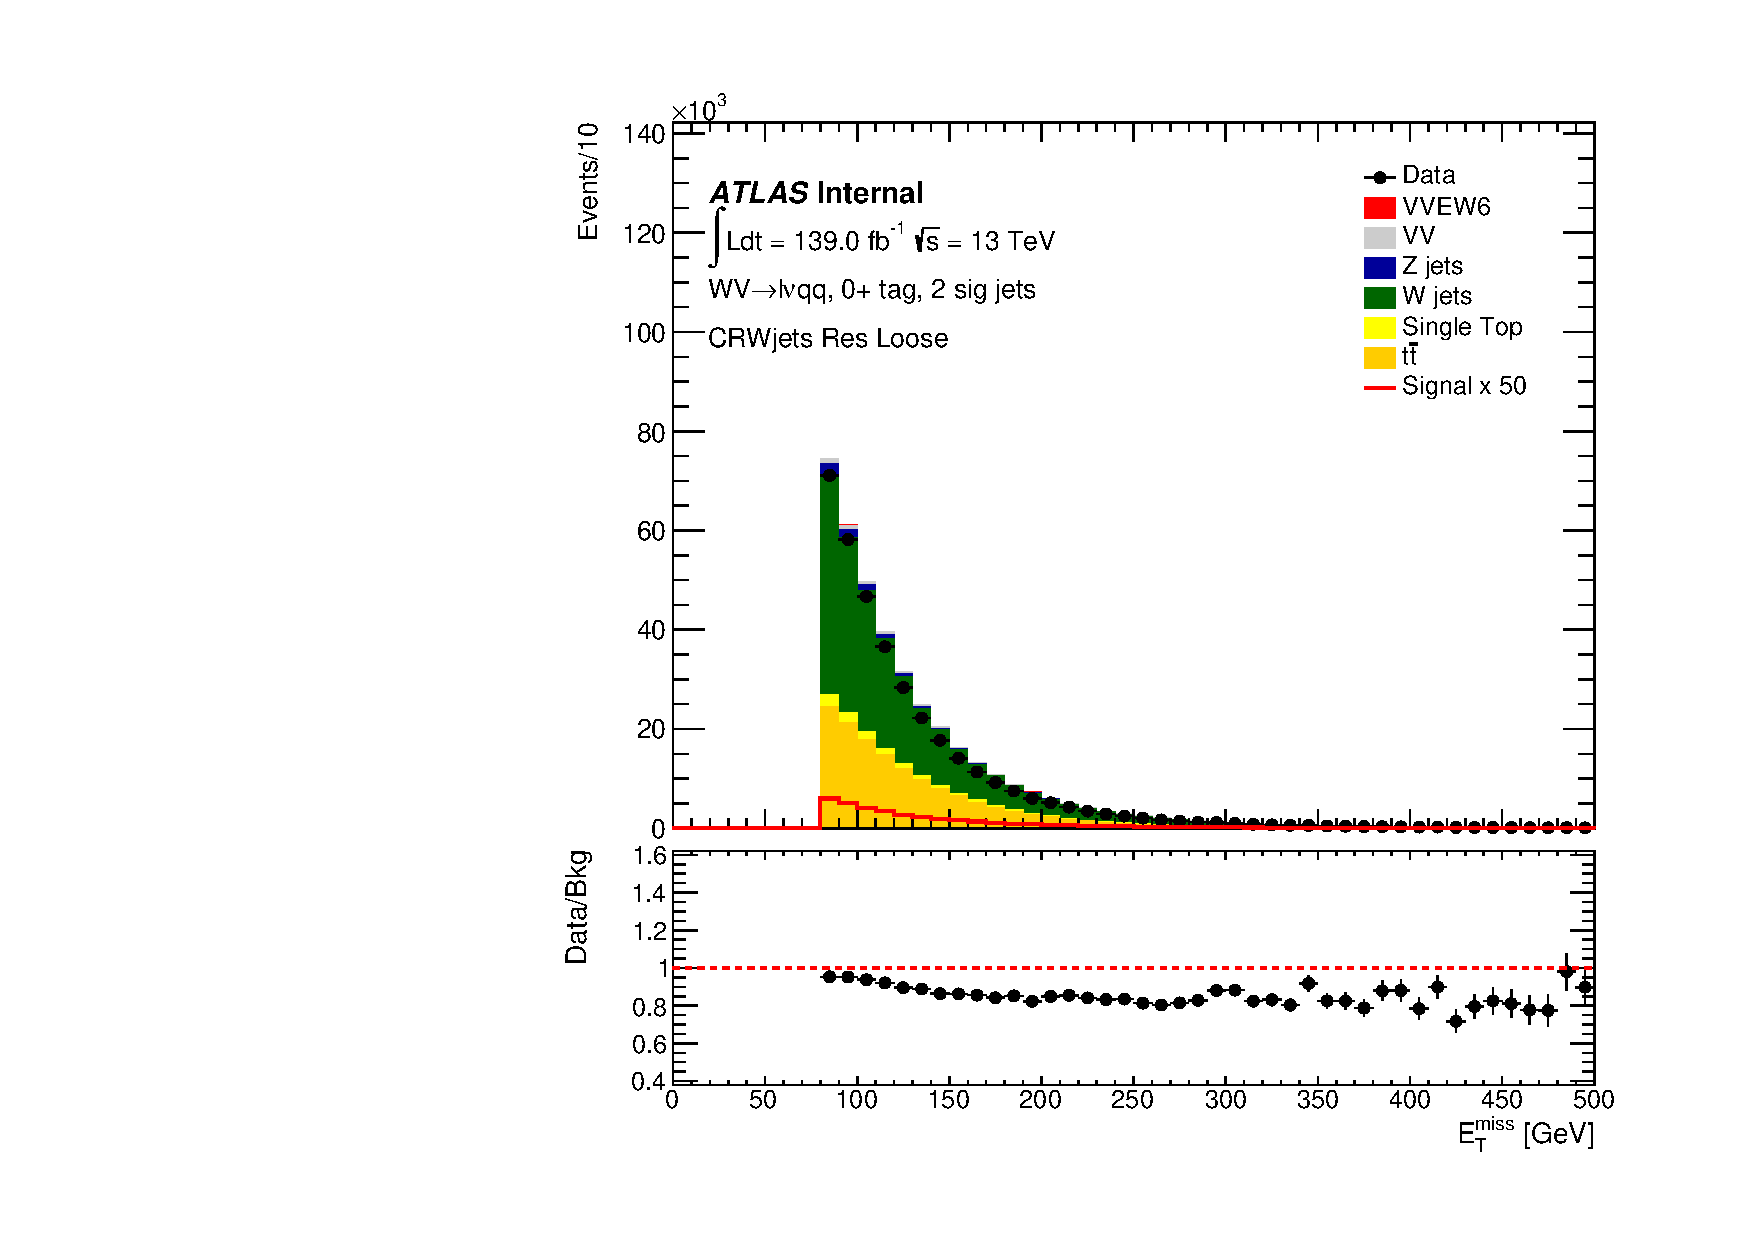
\includegraphics[width=0.3\textwidth]{figures/CRPlots/CRWjets_Res_Loose/stacked_plot_met.pdf}}  %%\\
%%    \subfloat[]{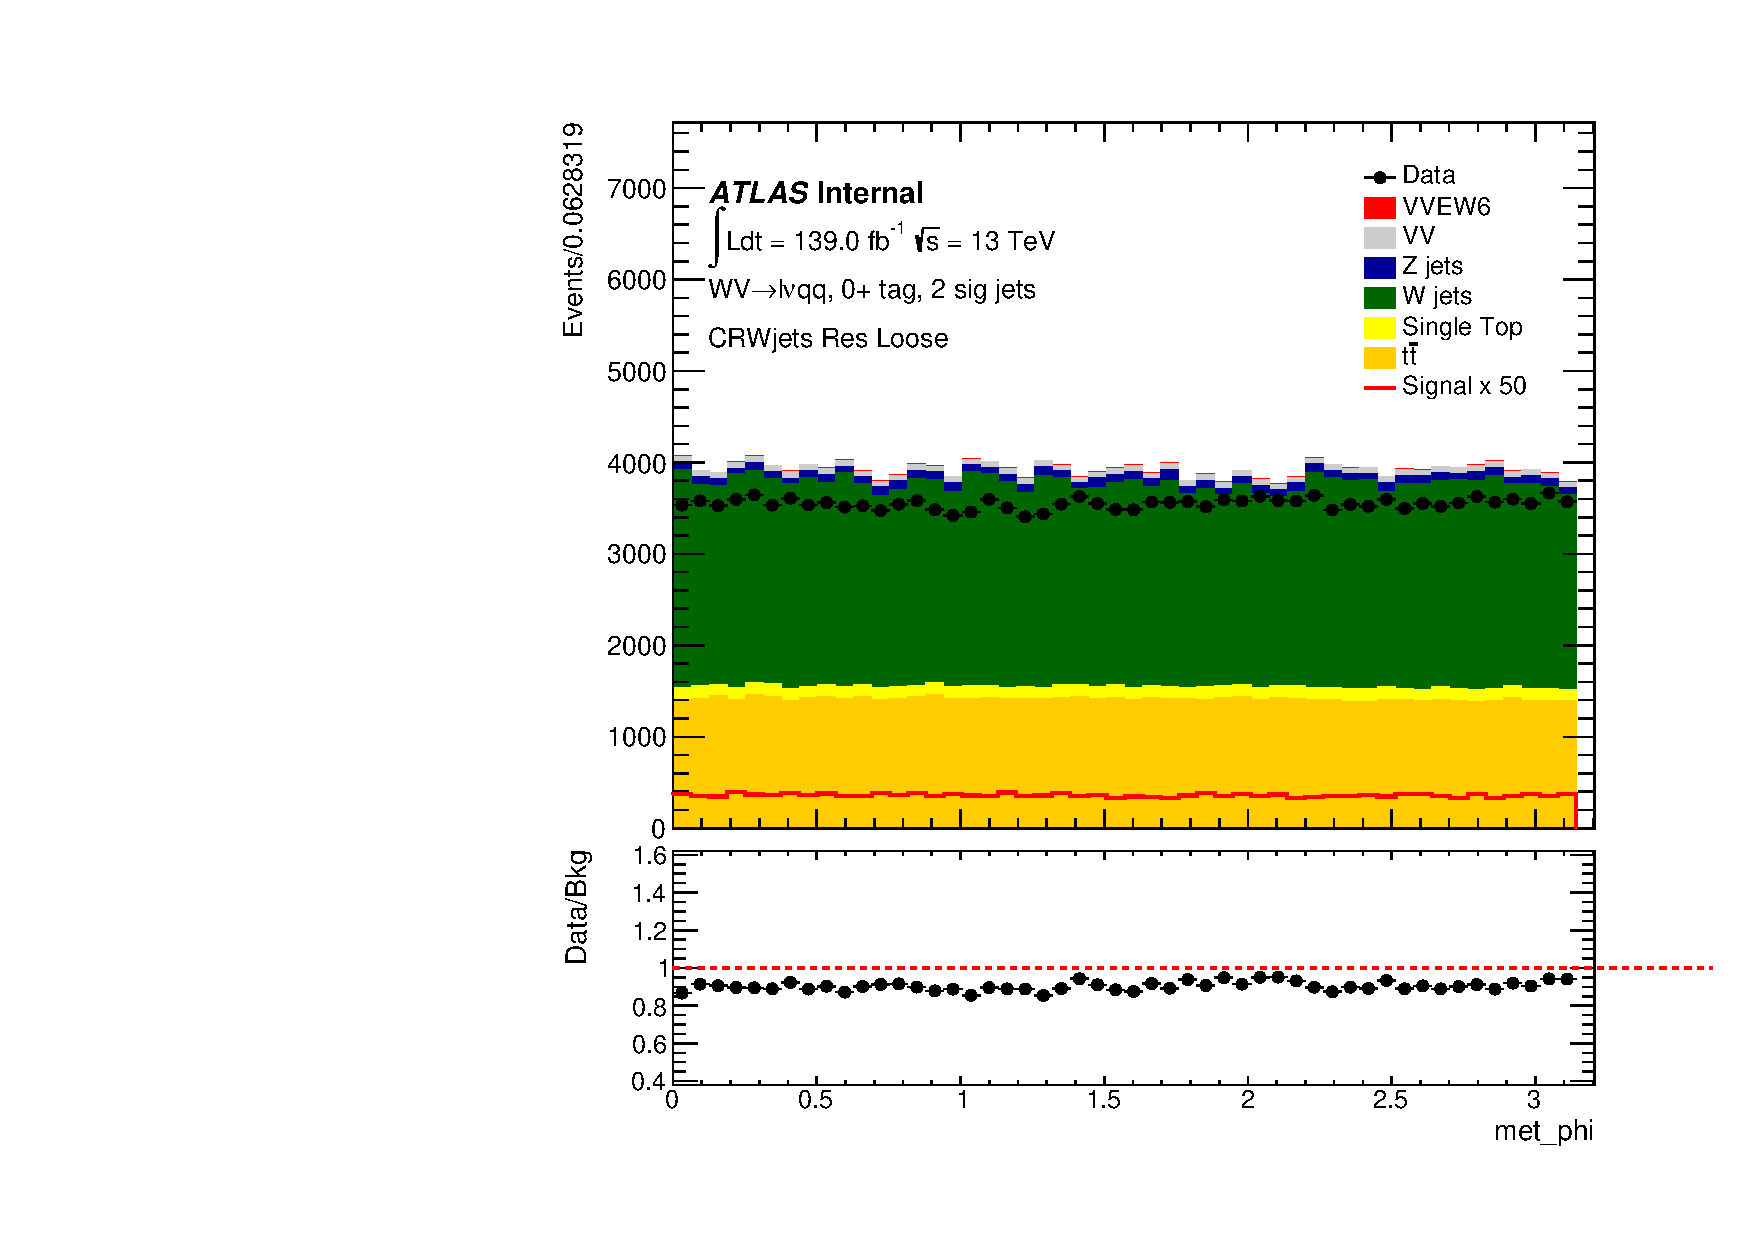
\includegraphics[width=0.3\textwidth]{figures/CRPlots/CRWjets_Res_Loose/stacked_plot_met_phi.pdf}}
%%    \subfloat[]{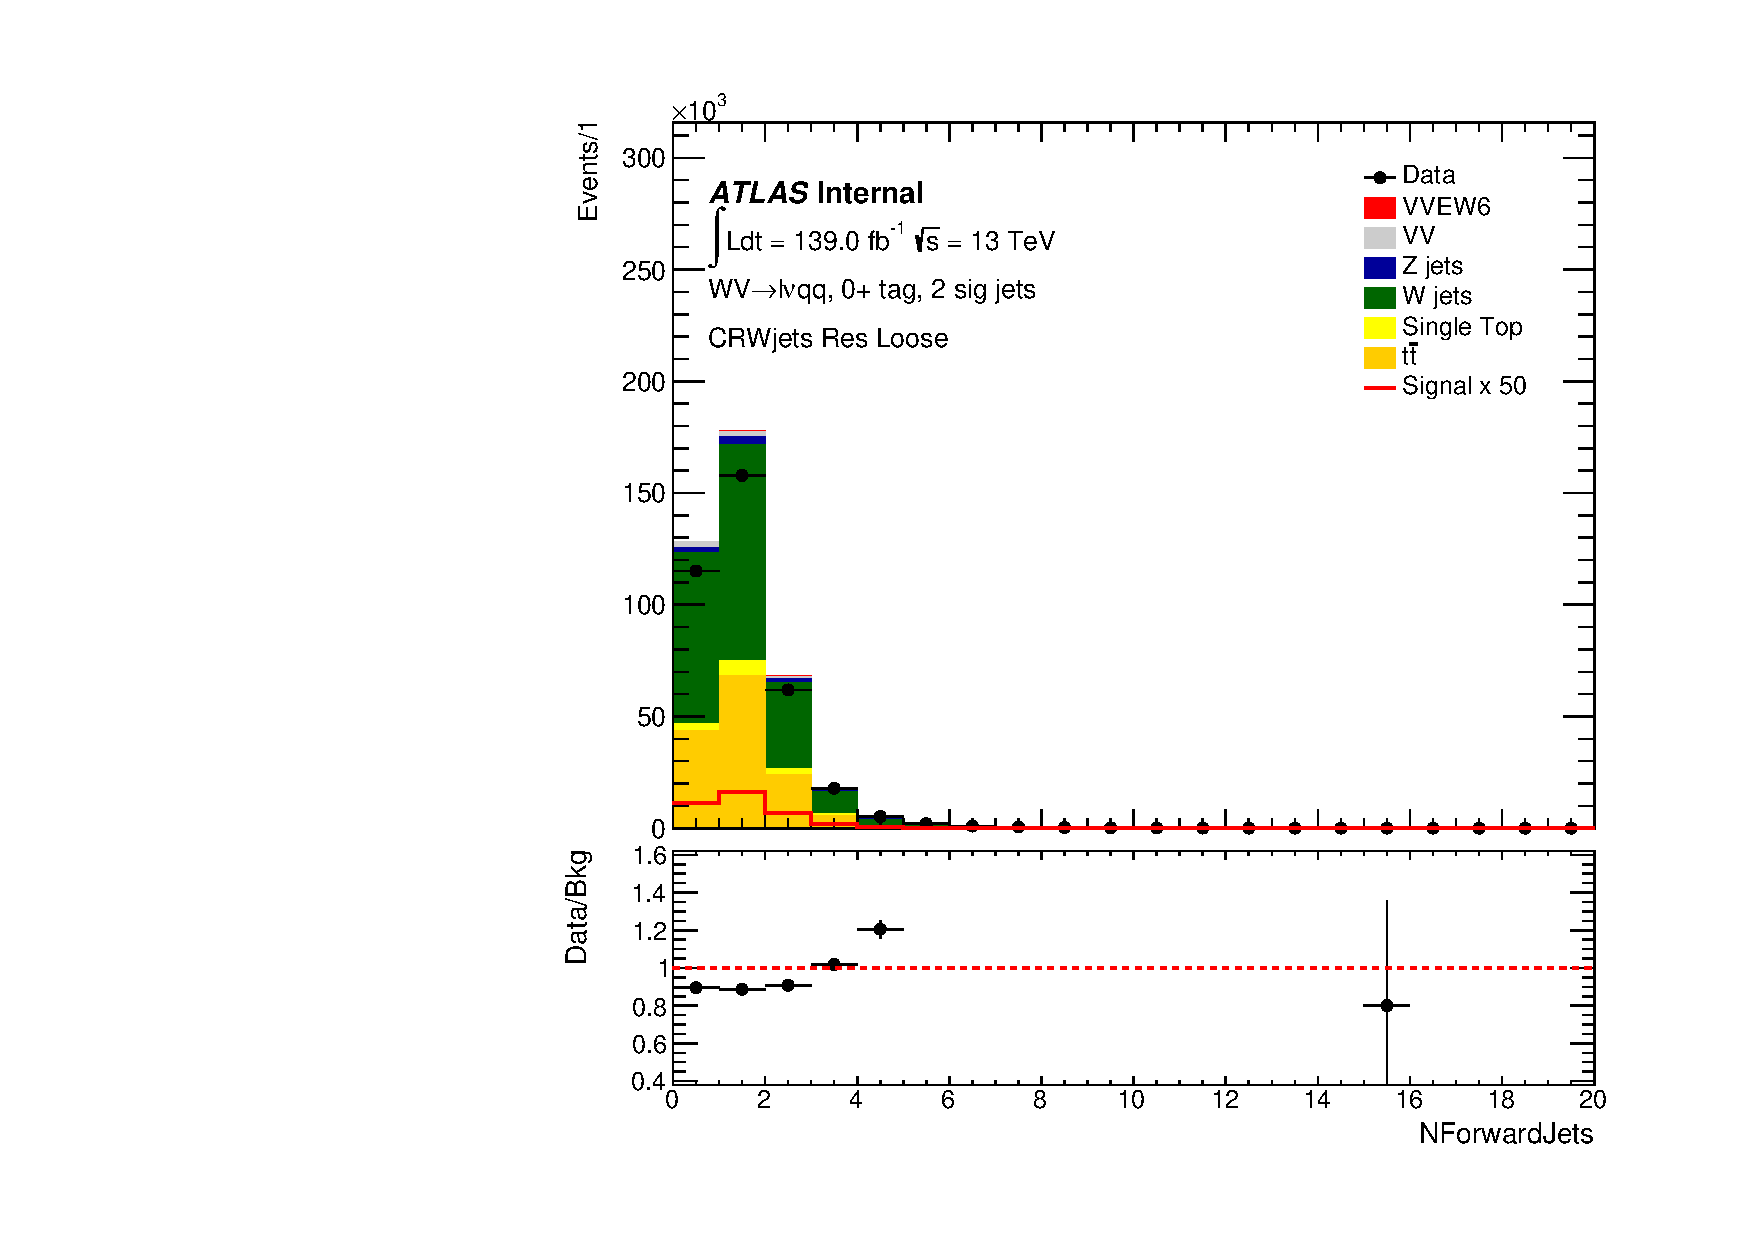
\includegraphics[width=0.3\textwidth]{figures/CRPlots/CRWjets_Res_Loose/stacked_plot_NForwardJets.pdf}}
    \caption{Data-MC checks for the resolved loose \Wjets control region in the \olep channel.}
    \label{fig:CRWjetResLoosePlots1Lep2}
\end{figure}

\begin{figure}[ht]
    \centering
    \subfloat[]{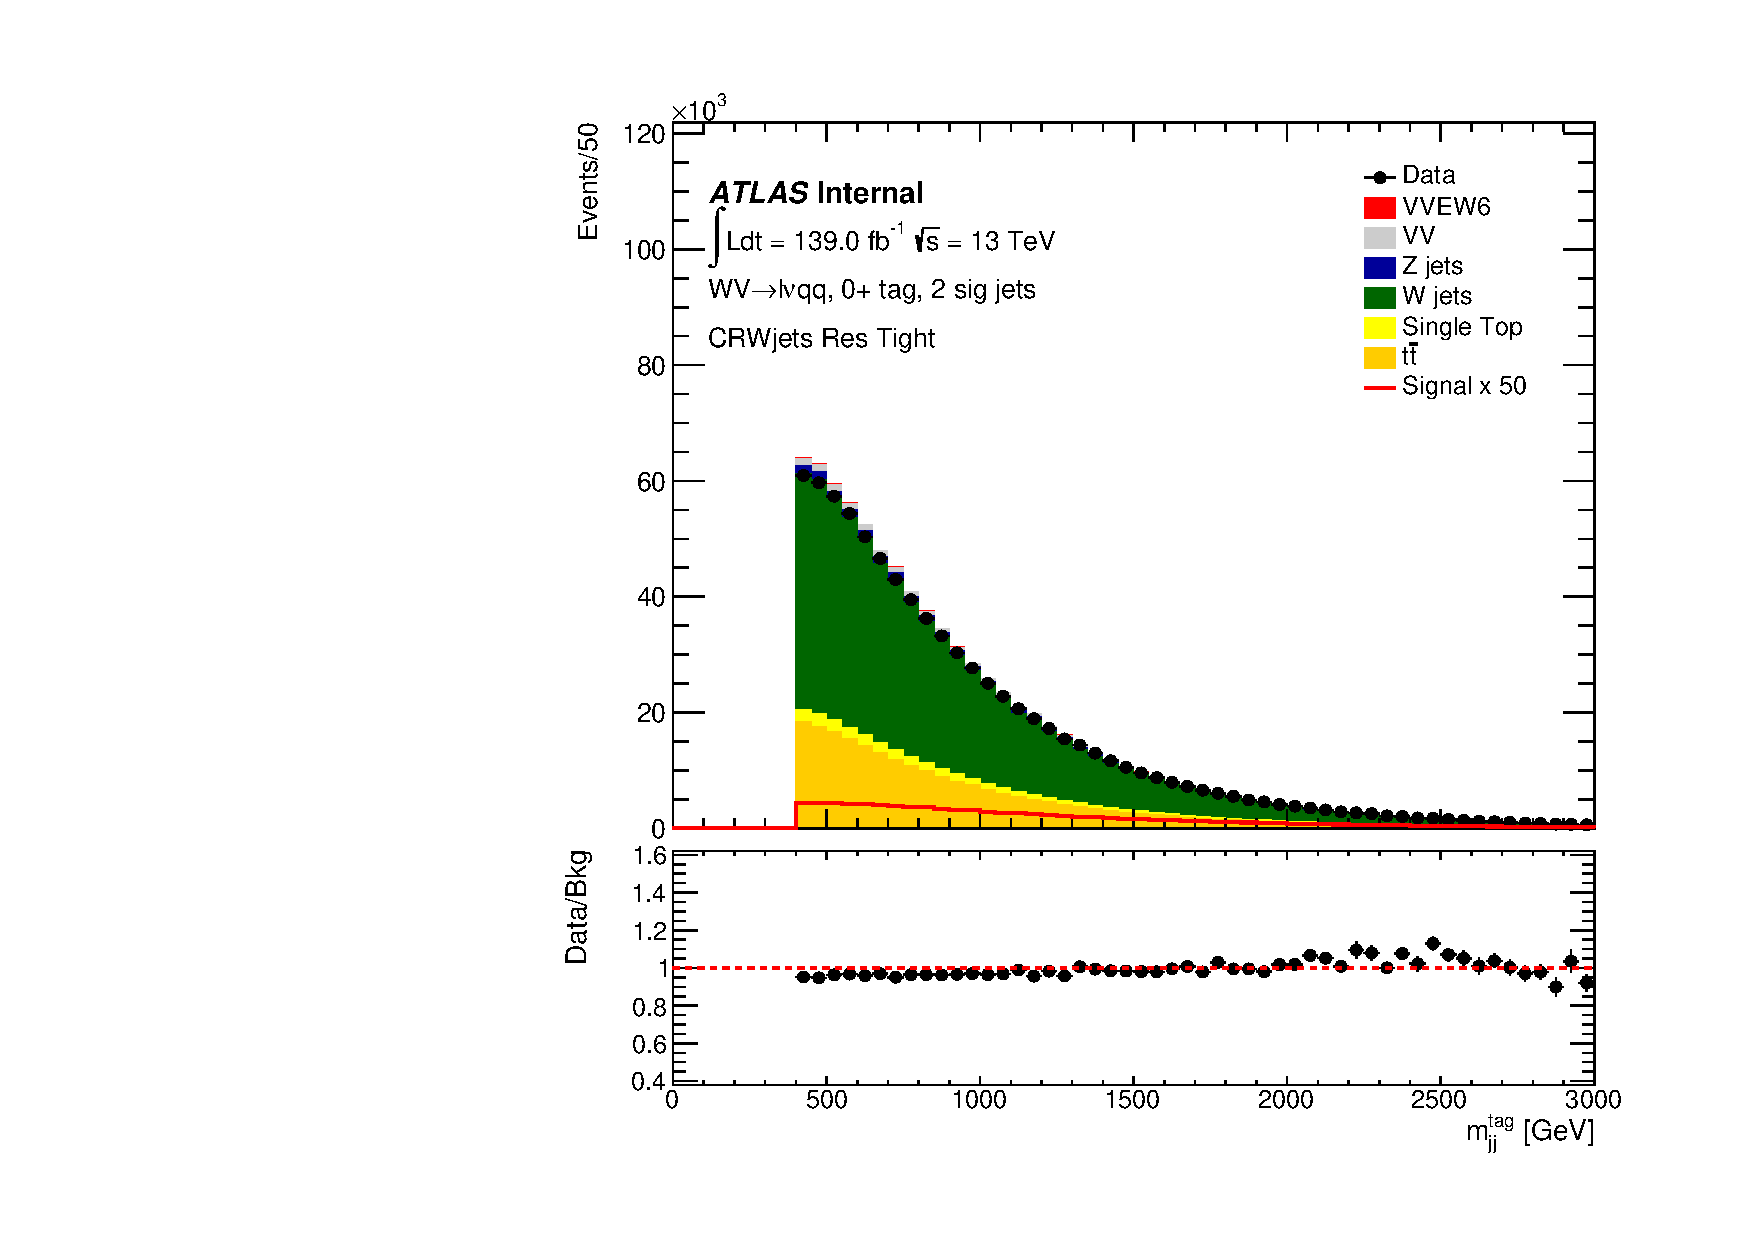
\includegraphics[width=0.3\textwidth]{figures/CRPlots/CRWjets_Res_Tight/stacked_plot_resolved_tagMjj.pdf}}
    \subfloat[]{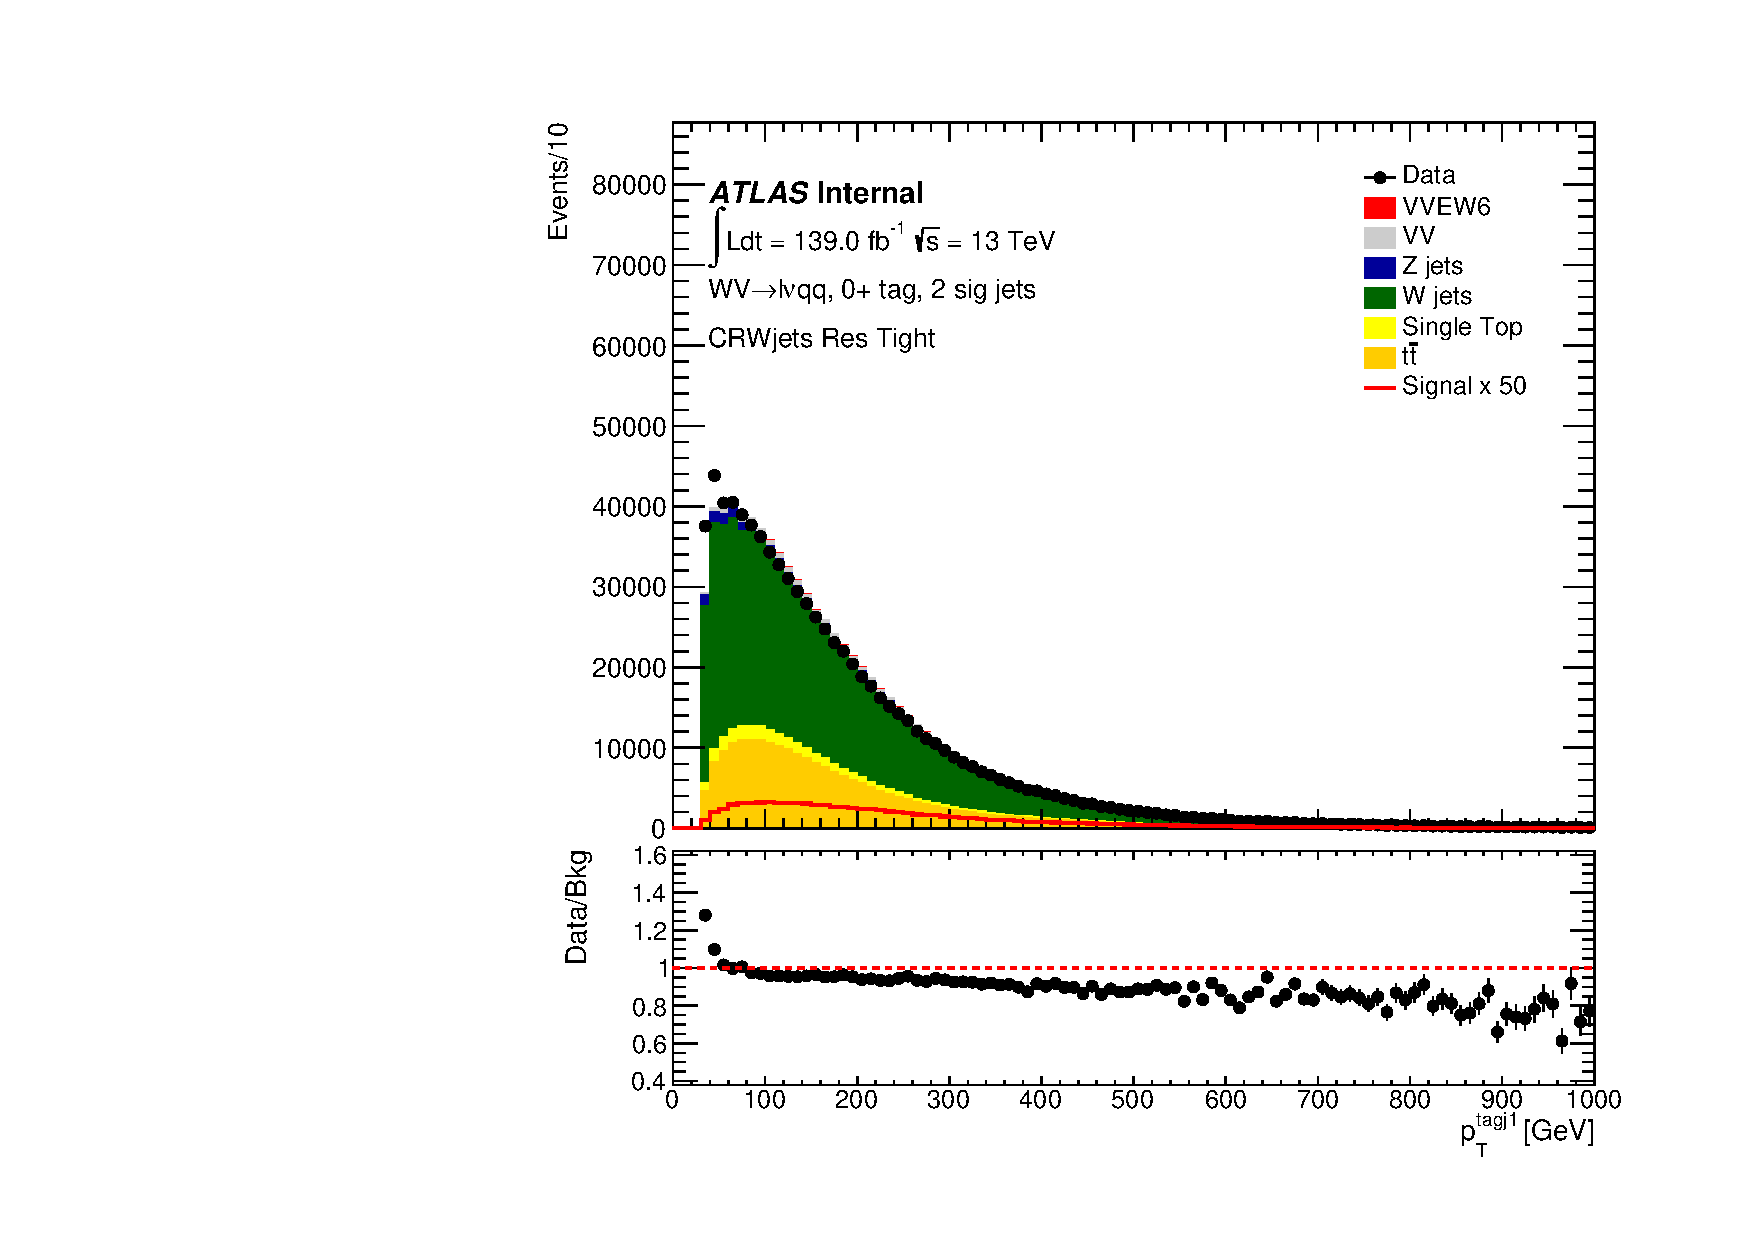
\includegraphics[width=0.3\textwidth]{figures/CRPlots/CRWjets_Res_Tight/stacked_plot_resolved_tagJ1_pt.pdf}}
    \subfloat[]{\includegraphics[width=0.3\textwidth]{figures/CRPlots/CRWjets_Res_Tight/stacked_plot_resolved_tagJ2_pt.pdf}} \\
    \subfloat[]{\includegraphics[width=0.3\textwidth]{figures/CRPlots/CRWjets_Res_Tight/stacked_plot_resolved_tagJ1_eta.pdf}}
    \subfloat[]{\includegraphics[width=0.3\textwidth]{figures/CRPlots/CRWjets_Res_Tight/stacked_plot_resolved_tagJ2_eta.pdf}} \\
    \subfloat[]{\includegraphics[width=0.3\textwidth]{figures/CRPlots/CRWjets_Res_Tight/stacked_plot_NJets.pdf}}
    \subfloat[]{\includegraphics[width=0.3\textwidth]{figures/CRPlots/CRWjets_Res_Tight/stacked_plot_NBJets.pdf}}
    \subfloat[]{\includegraphics[width=0.3\textwidth]{figures/CRPlots/CRWjets_Res_Tight/stacked_plot_lep_pt.pdf}}  %%\\
    \caption{Data-MC checks for the resolved tight \Wjets control region in the \olep channel.}
    \label{fig:CRWjetResTightPlots1Lep}
\end{figure}


\begin{figure}[ht]
    \centering
    \subfloat[]{\includegraphics[width=0.3\textwidth]{figures/CRPlots/CRWjets_Res_Tight/stacked_plot_W_m.pdf}}
    \subfloat[]{\includegraphics[width=0.3\textwidth]{figures/CRPlots/CRWjets_Res_Tight/stacked_plot_W_pt.pdf}}
    \subfloat[]{\includegraphics[width=0.3\textwidth]{figures/CRPlots/CRWjets_Res_Tight/stacked_plot_W_eta.pdf}} \\
    \subfloat[]{\includegraphics[width=0.3\textwidth]{figures/CRPlots/CRWjets_Res_Tight/stacked_plot_resolved_tagJdEta.pdf}}
    \subfloat[]{\includegraphics[width=0.3\textwidth]{figures/CRPlots/CRWjets_Res_Tight/stacked_plot_sigJ1_pt.pdf}}
    \subfloat[]{\includegraphics[width=0.3\textwidth]{figures/CRPlots/CRWjets_Res_Tight/stacked_plot_sigJ2_pt.pdf}} \\
    \subfloat[]{\includegraphics[width=0.3\textwidth]{figures/CRPlots/CRWjets_Res_Tight/stacked_plot_sigJ1_eta.pdf}}
    \subfloat[]{\includegraphics[width=0.3\textwidth]{figures/CRPlots/CRWjets_Res_Tight/stacked_plot_sigJ2_eta.pdf}} \\
    \subfloat[]{\includegraphics[width=0.3\textwidth]{figures/CRPlots/CRWjets_Res_Tight/stacked_plot_lvjjjjmass.pdf}}
    \subfloat[]{\includegraphics[width=0.3\textwidth]{figures/CRPlots/CRWjets_Res_Tight/stacked_plot_lvjjmass.pdf}}
    \subfloat[]{\includegraphics[width=0.3\textwidth]{figures/CRPlots/CRWjets_Res_Tight/stacked_plot_met.pdf}}  %%\\
%%    \subfloat[]{\includegraphics[width=0.3\textwidth]{figures/CRPlots/CRWjets_Res_Tight/stacked_plot_met_phi.pdf}}
%%    \subfloat[]{\includegraphics[width=0.3\textwidth]{figures/CRPlots/CRWjets_Res_Tight/stacked_plot_NForwardJets.pdf}}
    \caption{Data-MC checks for the resolved tight \Wjets control region in the \olep channel.}
    \label{fig:CRWjetResTightPlots1Lep2}
\end{figure}

\begin{figure}[ht]
    \centering
    \subfloat[]{\includegraphics[width=0.3\textwidth]{figures/CRPlots/CRWjets100/stacked_plot_merged_tagMjj.pdf}}
    \subfloat[]{\includegraphics[width=0.3\textwidth]{figures/CRPlots/CRWjets100/stacked_plot_merged_tagJ1_pt.pdf}}
    \subfloat[]{\includegraphics[width=0.3\textwidth]{figures/CRPlots/CRWjets100/stacked_plot_merged_tagJ2_pt.pdf}} \\
    \subfloat[]{\includegraphics[width=0.3\textwidth]{figures/CRPlots/CRWjets100/stacked_plot_merged_tagJ1_eta.pdf}}
    \subfloat[]{\includegraphics[width=0.3\textwidth]{figures/CRPlots/CRWjets100/stacked_plot_merged_tagJ2_eta.pdf}}
    \subfloat[]{\includegraphics[width=0.3\textwidth]{figures/CRPlots/CRWjets100/stacked_plot_fatJ_eta.pdf}} \\
    \subfloat[]{\includegraphics[width=0.3\textwidth]{figures/CRPlots/CRWjets100/stacked_plot_NJets.pdf}}
    \subfloat[]{\includegraphics[width=0.3\textwidth]{figures/CRPlots/CRWjets100/stacked_plot_NBJets.pdf}}
    \subfloat[]{\includegraphics[width=0.3\textwidth]{figures/CRPlots/CRWjets100/stacked_plot_lep_pt.pdf}}  \\
    \subfloat[]{\includegraphics[width=0.3\textwidth]{figures/CRPlots/CRWjets100/stacked_plot_fatJ_m.pdf}}
    \subfloat[]{\includegraphics[width=0.3\textwidth]{figures/CRPlots/CRWjets100/stacked_plot_fatJ_pt.pdf}}
    \subfloat[]{\includegraphics[width=0.3\textwidth]{figures/CRPlots/CRWjets100/stacked_plot_fatJ_D2.pdf}}
    \caption{Data-MC checks for the merged \Wjets control region in the \olep channel.}
    \label{fig:CRWjetMerPlots1Lep}
\end{figure}

\begin{figure}[ht]
    \centering
    \subfloat[]{\includegraphics[width=0.3\textwidth]{figures/CRPlots/CRWjets100/stacked_plot_W_m.pdf}}
    \subfloat[]{\includegraphics[width=0.3\textwidth]{figures/CRPlots/CRWjets100/stacked_plot_W_pt.pdf}}
    \subfloat[]{\includegraphics[width=0.3\textwidth]{figures/CRPlots/CRWjets100/stacked_plot_W_eta.pdf}} \\
    \subfloat[]{\includegraphics[width=0.3\textwidth]{figures/CRPlots/CRWjets100/stacked_plot_merged_tagJdEta.pdf}}
    \subfloat[]{\includegraphics[width=0.3\textwidth]{figures/CRPlots/CRWjets100/stacked_plot_fatJ_dRj1.pdf}}
    \subfloat[]{\includegraphics[width=0.3\textwidth]{figures/CRPlots/CRWjets100/stacked_plot_fatJ_dRj2.pdf}} \\
    \subfloat[]{\includegraphics[width=0.3\textwidth]{figures/CRPlots/CRWjets100/stacked_plot_lvJjjmass.pdf}}
    \subfloat[]{\includegraphics[width=0.3\textwidth]{figures/CRPlots/CRWjets100/stacked_plot_lvJmass.pdf}} \\
    \caption{Data-MC checks for the merged \Wjets control region in the \olep channel.}
    \label{fig:CRWjetMerPlots1Lep2}
\end{figure}

%%%

%%\begin{figure}[ht]
%%    \centering
%%    \subfigure[]{\includegraphics[width=0.3\textwidth]{figures/CRPlots/WjetsCR/C_0ptag1pfat0pjet_0ptv_CRVjet_Merged_Mer_tagMjj_Lin.pdf}}
%%    \subfigure[]{\includegraphics[width=0.3\textwidth]{figures/CRPlots/WjetsCR/C_0ptag1pfat0pjet_0ptv_CRVjet_Merged_PtTagMerJet1_Lin.pdf}}
%%    \subfigure[]{\includegraphics[width=0.3\textwidth]{figures/CRPlots/WjetsCR/C_0ptag1pfat0pjet_0ptv_CRVjet_Merged_PtTagMerJet2_Lin.pdf}} \\
%%    \subfigure[]{\includegraphics[width=0.3\textwidth]{figures/CRPlots/WjetsCR/C_0ptag1pfat0pjet_0ptv_CRVjet_Merged_EtaTagMerJet1_Lin.pdf}}
%%    \subfigure[]{\includegraphics[width=0.3\textwidth]{figures/CRPlots/WjetsCR/C_0ptag1pfat0pjet_0ptv_CRVjet_Merged_EtaTagMerJet2_Lin.pdf}}
%%    \subfigure[]{\includegraphics[width=0.3\textwidth]{figures/CRPlots/WjetsCR/C_0ptag1pfat0pjet_0ptv_CRVjet_Merged_EtaFatJet_Lin.pdf}}\\
%%    \subfigure[]{\includegraphics[width=0.3\textwidth]{figures/CRPlots/WjetsCR/C_0ptag1pfat0pjet_0ptv_CRVjet_Merged_NJets_Lin.pdf}}
%%    \subfigure[]{\includegraphics[width=0.3\textwidth]{figures/CRPlots/WjetsCR/C_0ptag1pfat0pjet_0ptv_CRVjet_Merged_NBJets_Lin.pdf}}
%%    \subfigure[]{\includegraphics[width=0.3\textwidth]{figures/CRPlots/WjetsCR/C_0ptag1pfat0pjet_0ptv_CRVjet_Merged_PtL_Lin.pdf}} \\
%%    \subfigure[]{\includegraphics[width=0.3\textwidth]{figures/CRPlots/WjetsCR/C_0ptag1pfat0pjet_0ptv_CRVjet_Merged_MFatJet_Lin.pdf}}
%%    \subfigure[]{\includegraphics[width=0.3\textwidth]{figures/CRPlots/WjetsCR/C_0ptag1pfat0pjet_0ptv_CRVjet_Merged_PtFatJet_Lin.pdf}}
%%    \subfigure[]{\includegraphics[width=0.3\textwidth]{figures/CRPlots/WjetsCR/C_0ptag1pfat0pjet_0ptv_CRVjet_Merged_D2FatJet_Lin.pdf}}
%%    \caption{Data-MC checks for the merged \Wjets control region in the \olep channel, after \mjjtag reweighting has been applied.}
%%    \label{fig:CRVjetMerPlots1Lep}
%%\end{figure}
%%
%%\begin{figure}[ht]
%%    \centering
%%    \subfigure[]{\includegraphics[width=0.3\textwidth]{figures/CRPlots/WjetsCR/C_0ptag1pfat0pjet_0ptv_CRVjet_Merged_MW_Lin.pdf}}
%%    \subfigure[]{\includegraphics[width=0.3\textwidth]{figures/CRPlots/WjetsCR/C_0ptag1pfat0pjet_0ptv_CRVjet_Merged_PtW_Lin.pdf}}
%%    \subfigure[]{\includegraphics[width=0.3\textwidth]{figures/CRPlots/WjetsCR/C_0ptag1pfat0pjet_0ptv_CRVjet_Merged_EtaW_Lin.pdf}} \\
%%    \subfigure[]{\includegraphics[width=0.3\textwidth]{figures/CRPlots/WjetsCR/C_0ptag1pfat0pjet_0ptv_CRVjet_Merged_DPhiTagMerJet_Lin.pdf}}
%%    \subfigure[]{\includegraphics[width=0.3\textwidth]{figures/CRPlots/WjetsCR/C_0ptag1pfat0pjet_0ptv_CRVjet_Merged_DEtaTagMerJet_Lin.pdf}} \\
%%    \subfigure[]{\includegraphics[width=0.3\textwidth]{figures/CRPlots/WjetsCR/C_0ptag1pfat0pjet_0ptv_CRVjet_Merged_DRFatJetTagJet1_Lin.pdf}}
%%    \subfigure[]{\includegraphics[width=0.3\textwidth]{figures/CRPlots/WjetsCR/C_0ptag1pfat0pjet_0ptv_CRVjet_Merged_DRFatJetTagJet2_Lin.pdf}}
%%    \subfigure[]{\includegraphics[width=0.3\textwidth]{figures/CRPlots/WjetsCR/C_0ptag1pfat0pjet_0ptv_CRVjet_Merged_DRFatJetTagjj_Lin.pdf}}
%%
%%    \caption{Data-MC checks for the merged \Wjets control region in the \olep channel, after \mjjtag reweighting has been applied.}
%%    \label{fig:CRVjetMerPlots1Lep2}
%%\end{figure}

%%\begin{figure}[ht]
%%    \centering
%%    \subfigure[]{\includegraphics[width=0.3\textwidth]{figures/CRPlots/WjetsCR/C_0ptag2pjet_0ptv_CRVjet_Res_tagMjj_Lin.pdf}}
%%    \subfigure[]{\includegraphics[width=0.3\textwidth]{figures/CRPlots/WjetsCR/C_0ptag2pjet_0ptv_CRVjet_PtTagResJet1_Lin.pdf}}
%%    \subfigure[]{\includegraphics[width=0.3\textwidth]{figures/CRPlots/WjetsCR/C_0ptag2pjet_0ptv_CRVjet_PtTagResJet2_Lin.pdf}} \\
%%    \subfigure[]{\includegraphics[width=0.3\textwidth]{figures/CRPlots/WjetsCR/C_0ptag2pjet_0ptv_CRVjet_EtaTagResJet1_Lin.pdf}}
%%    \subfigure[]{\includegraphics[width=0.3\textwidth]{figures/CRPlots/WjetsCR/C_0ptag2pjet_0ptv_CRVjet_EtaTagResJet2_Lin.pdf}} \\
%%    \subfigure[]{\includegraphics[width=0.3\textwidth]{figures/CRPlots/WjetsCR/C_0ptag2pjet_0ptv_CRVjet_NJets_Lin.pdf}}
%%    \subfigure[]{\includegraphics[width=0.3\textwidth]{figures/CRPlots/WjetsCR/C_0ptag2pjet_0ptv_CRVjet_NBJets_Lin.pdf}}
%%    \subfigure[]{\includegraphics[width=0.3\textwidth]{figures/CRPlots/WjetsCR/C_0ptag2pjet_0ptv_CRVjet_PtL_Lin.pdf}}  \\
%%    \subfigure[]{\includegraphics[width=0.3\textwidth]{figures/CRPlots/WjetsCR/C_0ptag2pjet_0ptv_CRVjet_MW_Lin.pdf}}
%%    \subfigure[]{\includegraphics[width=0.3\textwidth]{figures/CRPlots/WjetsCR/C_0ptag2pjet_0ptv_CRVjet_PtW_Lin.pdf}}
%%    \subfigure[]{\includegraphics[width=0.3\textwidth]{figures/CRPlots/WjetsCR/C_0ptag2pjet_0ptv_CRVjet_EtaW_Lin.pdf}}
%%    \caption{Data-MC checks for the resolved loose \Wjets control region in the \olep channel, after \mjjtag reweighting has been applied.}
%%    \label{fig:CRVjetResLoosePlots1Lep}
%%\end{figure}
%%
%%\begin{figure}[ht]
%%    \centering
%%    \subfigure[]{\includegraphics[width=0.3\textwidth]{figures/CRPlots/WjetsCR/C_0ptag2pjet_0ptv_CRVjet_DPhiTagResJet_Lin.pdf}}
%%    \subfigure[]{\includegraphics[width=0.3\textwidth]{figures/CRPlots/WjetsCR/C_0ptag2pjet_0ptv_CRVjet_DEtaTagResJet_Lin.pdf}} \\
%%    \subfigure[]{\includegraphics[width=0.3\textwidth]{figures/CRPlots/WjetsCR/C_0ptag2pjet_0ptv_CRVjet_DRSigjjTagJet1_Lin.pdf}}
%%    \subfigure[]{\includegraphics[width=0.3\textwidth]{figures/CRPlots/WjetsCR/C_0ptag2pjet_0ptv_CRVjet_DRSigjjTagJet2_Lin.pdf}}
%%    \subfigure[]{\includegraphics[width=0.3\textwidth]{figures/CRPlots/WjetsCR/C_0ptag2pjet_0ptv_CRVjet_DRSigjjTagjj_Lin.pdf}} \\
%%    \subfigure[]{\includegraphics[width=0.3\textwidth]{figures/CRPlots/WjetsCR/C_0ptag2pjet_0ptv_CRVjet_EtaSigJet1_Lin.pdf}}
%%    \subfigure[]{\includegraphics[width=0.3\textwidth]{figures/CRPlots/WjetsCR/C_0ptag2pjet_0ptv_CRVjet_EtaSigJet2_Lin.pdf}}
%%    \caption{Data-MC checks for the resolved loose \Wjets control region in the \olep channel, after \mjjtag reweighting has been applied.}
%%    \label{fig:CRVjetResLoosePlots1Lep2}
%%\end{figure}


%%%
%%\input{source/bkg_modelling/ZjetsCR}
%%%
%%\input{source/bkg_modelling/VjetsCR}
%%%
\clearpage
\section{Top Background Control Region}
%%\clearpage
%%\subsection{Top control region}
%%\label{subsec:top_cr}

Figures
\ref{fig:CRTopResLoosePlots1Lep}
\ref{fig:CRTopResTightPlots1Lep}
\ref{fig:CRTopMerLPPlots1Lep}
\ref{fig:CRTopMerHPPlots1Lep}
show the main relevant kinematic variable distributions in the Top CR in \olep channel, after \mjjtag reweighting has been applied.

\begin{figure}[ht]
    \centering
    \subfloat[]{\includegraphics[width=0.3\textwidth]{figures/CRPlots/CRTop_Res_Loose/stacked_plot_resolved_tagMjj.pdf}}
    \subfloat[]{\includegraphics[width=0.3\textwidth]{figures/CRPlots/CRTop_Res_Loose/stacked_plot_resolved_tagJ1_pt.pdf}}
    \subfloat[]{\includegraphics[width=0.3\textwidth]{figures/CRPlots/CRTop_Res_Loose/stacked_plot_resolved_tagJ2_pt.pdf}} \\
    \subfloat[]{\includegraphics[width=0.3\textwidth]{figures/CRPlots/CRTop_Res_Loose/stacked_plot_resolved_tagJ1_eta.pdf}}
    \subfloat[]{\includegraphics[width=0.3\textwidth]{figures/CRPlots/CRTop_Res_Loose/stacked_plot_resolved_tagJ2_eta.pdf}} \\
    \subfloat[]{\includegraphics[width=0.3\textwidth]{figures/CRPlots/CRTop_Res_Loose/stacked_plot_NJets.pdf}}
    \subfloat[]{\includegraphics[width=0.3\textwidth]{figures/CRPlots/CRTop_Res_Loose/stacked_plot_NBJets.pdf}}
    \subfloat[]{\includegraphics[width=0.3\textwidth]{figures/CRPlots/CRTop_Res_Loose/stacked_plot_lep_pt.pdf}}
    \caption{Data-MC checks for the resolved loose top control region in the \olep channel.}
    \label{fig:CRTopResLoosePlots1Lep}
\end{figure}

\begin{figure}[ht]
    \centering
    \subfloat[]{\includegraphics[width=0.3\textwidth]{figures/CRPlots/CRTop_Res_Loose/stacked_plot_resolved_tagJdEta.pdf}}
    \subfloat[]{\includegraphics[width=0.3\textwidth]{figures/CRPlots/CRTop_Res_Loose/stacked_plot_sigJ1_pt.pdf}}
    \subfloat[]{\includegraphics[width=0.3\textwidth]{figures/CRPlots/CRTop_Res_Loose/stacked_plot_sigJ2_pt.pdf}} \\
    \subfloat[]{\includegraphics[width=0.3\textwidth]{figures/CRPlots/CRTop_Res_Loose/stacked_plot_sigJ1_eta.pdf}}
    \subfloat[]{\includegraphics[width=0.3\textwidth]{figures/CRPlots/CRTop_Res_Loose/stacked_plot_sigJ2_eta.pdf}} \\
    \subfloat[]{\includegraphics[width=0.3\textwidth]{figures/CRPlots/CRTop_Res_Loose/stacked_plot_lvjjjjmass.pdf}}
    \subfloat[]{\includegraphics[width=0.3\textwidth]{figures/CRPlots/CRTop_Res_Loose/stacked_plot_lvjjmass.pdf}}
    \subfloat[]{\includegraphics[width=0.3\textwidth]{figures/CRPlots/CRTop_Res_Loose/stacked_plot_met.pdf}}  \\
    \caption{Data-MC checks for the resolved loose top control region in the \olep channel.}
    \label{fig:CRTopResLoosePlots1Lep2}
\end{figure}

\begin{figure}[ht]
    \centering
    \subfloat[]{\includegraphics[width=0.3\textwidth]{figures/CRPlots/CRTop_Res_Tight/stacked_plot_resolved_tagMjj.pdf}}
    \subfloat[]{\includegraphics[width=0.3\textwidth]{figures/CRPlots/CRTop_Res_Tight/stacked_plot_resolved_tagJ1_pt.pdf}}
    \subfloat[]{\includegraphics[width=0.3\textwidth]{figures/CRPlots/CRTop_Res_Tight/stacked_plot_resolved_tagJ2_pt.pdf}} \\
    \subfloat[]{\includegraphics[width=0.3\textwidth]{figures/CRPlots/CRTop_Res_Tight/stacked_plot_resolved_tagJ1_eta.pdf}}
    \subfloat[]{\includegraphics[width=0.3\textwidth]{figures/CRPlots/CRTop_Res_Tight/stacked_plot_resolved_tagJ2_eta.pdf}} \\
    \subfloat[]{\includegraphics[width=0.3\textwidth]{figures/CRPlots/CRTop_Res_Tight/stacked_plot_NJets.pdf}}
    \subfloat[]{\includegraphics[width=0.3\textwidth]{figures/CRPlots/CRTop_Res_Tight/stacked_plot_NBJets.pdf}}
    \subfloat[]{\includegraphics[width=0.3\textwidth]{figures/CRPlots/CRTop_Res_Tight/stacked_plot_lep_pt.pdf}}
    \caption{Data-MC checks for the resolved tight top control region in the \olep channel.}
    \label{fig:CRTopResTightPlots1Lep}
\end{figure}

\begin{figure}[ht]
    \centering
    \subfloat[]{\includegraphics[width=0.3\textwidth]{figures/CRPlots/CRTop_Res_Tight/stacked_plot_resolved_tagJdEta.pdf}}
    \subfloat[]{\includegraphics[width=0.3\textwidth]{figures/CRPlots/CRTop_Res_Tight/stacked_plot_sigJ1_pt.pdf}}
    \subfloat[]{\includegraphics[width=0.3\textwidth]{figures/CRPlots/CRTop_Res_Tight/stacked_plot_sigJ2_pt.pdf}} \\
    \subfloat[]{\includegraphics[width=0.3\textwidth]{figures/CRPlots/CRTop_Res_Tight/stacked_plot_sigJ1_eta.pdf}}
    \subfloat[]{\includegraphics[width=0.3\textwidth]{figures/CRPlots/CRTop_Res_Tight/stacked_plot_sigJ2_eta.pdf}} \\
    \subfloat[]{\includegraphics[width=0.3\textwidth]{figures/CRPlots/CRTop_Res_Tight/stacked_plot_lvjjjjmass.pdf}}
    \subfloat[]{\includegraphics[width=0.3\textwidth]{figures/CRPlots/CRTop_Res_Tight/stacked_plot_lvjjmass.pdf}}
    \subfloat[]{\includegraphics[width=0.3\textwidth]{figures/CRPlots/CRTop_Res_Tight/stacked_plot_met.pdf}}  \\
    \caption{Data-MC checks for the resolved tight top control region in the \olep channel.}
    \label{fig:CRTopResTightPlots1Lep2}
\end{figure}

\begin{figure}[ht]
    \centering
    \subfloat[]{\includegraphics[width=0.3\textwidth]{figures/CRPlots/CRTop_80/stacked_plot_merged_tagMjj.pdf}}
    \subfloat[]{\includegraphics[width=0.3\textwidth]{figures/CRPlots/CRTop_80/stacked_plot_merged_tagJ1_pt.pdf}}
    \subfloat[]{\includegraphics[width=0.3\textwidth]{figures/CRPlots/CRTop_80/stacked_plot_merged_tagJ2_pt.pdf}} \\
    \subfloat[]{\includegraphics[width=0.3\textwidth]{figures/CRPlots/CRTop_80/stacked_plot_merged_tagJ1_eta.pdf}}
    \subfloat[]{\includegraphics[width=0.3\textwidth]{figures/CRPlots/CRTop_80/stacked_plot_merged_tagJ2_eta.pdf}} \\
    \subfloat[]{\includegraphics[width=0.3\textwidth]{figures/CRPlots/CRTop_80/stacked_plot_NJets.pdf}}
    \subfloat[]{\includegraphics[width=0.3\textwidth]{figures/CRPlots/CRTop_80/stacked_plot_NBJets.pdf}}
    \subfloat[]{\includegraphics[width=0.3\textwidth]{figures/CRPlots/CRTop_80/stacked_plot_lep_pt.pdf}} \\
    \subfloat[]{\includegraphics[width=0.3\textwidth]{figures/CRPlots/CRTop_80/stacked_plot_fatJ_m.pdf}}
    \subfloat[]{\includegraphics[width=0.3\textwidth]{figures/CRPlots/CRTop_80/stacked_plot_fatJ_pt.pdf}}
    \subfloat[]{\includegraphics[width=0.3\textwidth]{figures/CRPlots/CRTop_80/stacked_plot_fatJ_D2.pdf}}
    \caption{Data-MC checks for the merged low-purity top control region in the \olep channel.}
    \label{fig:CRTopMerLPPlots1Lep}
\end{figure}

\begin{figure}[ht]
    \centering
    \subfloat[]{\includegraphics[width=0.3\textwidth]{figures/CRPlots/CRTop_80/stacked_plot_W_m.pdf}}
    \subfloat[]{\includegraphics[width=0.3\textwidth]{figures/CRPlots/CRTop_80/stacked_plot_W_pt.pdf}}
    \subfloat[]{\includegraphics[width=0.3\textwidth]{figures/CRPlots/CRTop_80/stacked_plot_W_eta.pdf}} \\
    \subfloat[]{\includegraphics[width=0.3\textwidth]{figures/CRPlots/CRTop_80/stacked_plot_merged_tagJdEta.pdf}}
    \subfloat[]{\includegraphics[width=0.3\textwidth]{figures/CRPlots/CRTop_80/stacked_plot_fatJ_dRj1.pdf}}
    \subfloat[]{\includegraphics[width=0.3\textwidth]{figures/CRPlots/CRTop_80/stacked_plot_fatJ_dRj2.pdf}} \\
    \subfloat[]{\includegraphics[width=0.3\textwidth]{figures/CRPlots/CRTop_80/stacked_plot_lvJjjmass.pdf}}
    \subfloat[]{\includegraphics[width=0.3\textwidth]{figures/CRPlots/CRTop_80/stacked_plot_lvJmass.pdf}} \\
    \caption{Data-MC checks for the merged low-purity top control region in the \olep channel.}
    \label{fig:CRTopMerLPPlots1Lep2}
\end{figure}

\begin{figure}[ht]
    \centering
    \subfloat[]{\includegraphics[width=0.3\textwidth]{figures/CRPlots/CRTop_50/stacked_plot_merged_tagMjj.pdf}}
    \subfloat[]{\includegraphics[width=0.3\textwidth]{figures/CRPlots/CRTop_50/stacked_plot_merged_tagJ1_pt.pdf}}
    \subfloat[]{\includegraphics[width=0.3\textwidth]{figures/CRPlots/CRTop_50/stacked_plot_merged_tagJ2_pt.pdf}} \\
    \subfloat[]{\includegraphics[width=0.3\textwidth]{figures/CRPlots/CRTop_50/stacked_plot_merged_tagJ1_eta.pdf}}
    \subfloat[]{\includegraphics[width=0.3\textwidth]{figures/CRPlots/CRTop_50/stacked_plot_merged_tagJ2_eta.pdf}} \\
    \subfloat[]{\includegraphics[width=0.3\textwidth]{figures/CRPlots/CRTop_50/stacked_plot_NJets.pdf}}
    \subfloat[]{\includegraphics[width=0.3\textwidth]{figures/CRPlots/CRTop_50/stacked_plot_NBJets.pdf}}
    \subfloat[]{\includegraphics[width=0.3\textwidth]{figures/CRPlots/CRTop_50/stacked_plot_lep_pt.pdf}} \\
    \subfloat[]{\includegraphics[width=0.3\textwidth]{figures/CRPlots/CRTop_50/stacked_plot_fatJ_m.pdf}}
    \subfloat[]{\includegraphics[width=0.3\textwidth]{figures/CRPlots/CRTop_50/stacked_plot_fatJ_pt.pdf}}
    \subfloat[]{\includegraphics[width=0.3\textwidth]{figures/CRPlots/CRTop_50/stacked_plot_fatJ_D2.pdf}}
    \caption{Data-MC checks for the merged high-purity top control region in the \olep channel.}
    \label{fig:CRTopMerHPPlots1Lep}
\end{figure}

\begin{figure}[ht]
    \centering
    \subfloat[]{\includegraphics[width=0.3\textwidth]{figures/CRPlots/CRTop_50/stacked_plot_W_m.pdf}}
    \subfloat[]{\includegraphics[width=0.3\textwidth]{figures/CRPlots/CRTop_50/stacked_plot_W_pt.pdf}}
    \subfloat[]{\includegraphics[width=0.3\textwidth]{figures/CRPlots/CRTop_50/stacked_plot_W_eta.pdf}} \\
    \subfloat[]{\includegraphics[width=0.3\textwidth]{figures/CRPlots/CRTop_50/stacked_plot_merged_tagJdEta.pdf}}
    \subfloat[]{\includegraphics[width=0.3\textwidth]{figures/CRPlots/CRTop_50/stacked_plot_fatJ_dRj1.pdf}}
    \subfloat[]{\includegraphics[width=0.3\textwidth]{figures/CRPlots/CRTop_50/stacked_plot_fatJ_dRj2.pdf}} \\
    \subfloat[]{\includegraphics[width=0.3\textwidth]{figures/CRPlots/CRTop_50/stacked_plot_lvJjjmass.pdf}}
    \subfloat[]{\includegraphics[width=0.3\textwidth]{figures/CRPlots/CRTop_50/stacked_plot_lvJmass.pdf}} \\
    \caption{Data-MC checks for the merged high-purity top control region in the \olep channel.}
    \label{fig:CRTopMerHPPlots1Lep2}
\end{figure}

%%%%%%%%%%

